% Minimal sebenta template generated automatically
\documentclass[11pt,a4paper]{article}
\usepackage[utf8]{inputenc}
\usepackage[T1]{fontenc}
\usepackage{lmodern}
\usepackage{geometry}
\usepackage{fancyhdr}
\usepackage{hyperref}
\usepackage{graphicx}
\usepackage{float}
\usepackage{placeins}
\usepackage{bookmark}
\usepackage{booktabs}
\usepackage{amsmath,amssymb}
\usepackage{csquotes}
\usepackage{enumitem}
\geometry{margin=2.5cm}

% Try to include project-specific style macros (containing \exercicio, \subexercicio, etc.)
% Try multiple relative locations to be robust across different generated output paths
\IfFileExists{../../../../Teste_modelo/config/style.tex}{% Sistema de exercícios com contadores automáticos
\newcounter{exerciciocount}          % Contador principal dos exercícios
\newcounter{subexerciciocount}       % Contador dos subexercícios
\newcounter{optioncount}             % Contador das opções

% Control whether the macro prints the automatic "Exercício N." heading.
% Default: show the heading. Call \showexerciciotitlefalse to suppress.
\newif\ifshowexerciciotitle
\showexerciciotitletrue

% Macro para exercício principal
\newcommand{\exercicio}[1]{%
        \par\vspace{1.5em}% Espaçamento antes
        \refstepcounter{exerciciocount}% Incrementa contador principal
        \setcounter{subexerciciocount}{0}% Reseta contador de subexercícios
        \setcounter{optioncount}{0}% Reseta contador de opções
        % Only print the automatic heading if the flag is true
        \ifshowexerciciotitle
            \noindent\textbf{Exercício~\theexerciciocount.}\space #1\par\vspace{0.5em}%
        \else
            % When suppressed, just print the content without the heading
            #1\par\vspace{0.5em}%
        \fi
}

% Macro para subexercício
\newcommand{\subexercicio}[1]{%
    \par\vspace{0.8em}% Espaçamento menor para subexercícios
    \refstepcounter{subexerciciocount}% Incrementa contador de subexercícios
    \noindent\textbf{\theexerciciocount.\thesubexerciciocount.} #1\par\vspace{0.3em}%
}

% Macro para opção
\newcommand{\option}[1]{%
    \par
    \refstepcounter{optioncount}%
    \noindent(\alph{optioncount}) #1%
}

% Título e informações do exame
\title{1ª Questão de aula do Módulo A10: Otimização}
\author{EPRALIMA - Escola Profissional Alto Lima}

\date{}

% Cabeçalho completo do teste dentro de uma caixa simples
\newcommand{\espacoAluno}{%
    \vspace{0.5cm}
    \fbox{%
        \parbox{\textwidth}{%
            \noindent\textbf{Nome do Aluno:} \underline{\hspace{7cm}} \textbf{Turma:} \underline{\hspace{1cm}}\\[0.5cm]
            \noindent\textbf{Assinatura do Professor:} \underline{\hspace{3cm}} \hfill \textbf{Nota:} \underline{\hspace{2cm}}\\[0.5cm]
            \noindent\textbf{Assinatura do Encarregado de Educação:} \underline{\hspace{3cm}}
        }%
    }
    \vspace{1cm}
}}{%
  \IfFileExists{../../../Teste_modelo/config/style.tex}{% Sistema de exercícios com contadores automáticos
\newcounter{exerciciocount}          % Contador principal dos exercícios
\newcounter{subexerciciocount}       % Contador dos subexercícios
\newcounter{optioncount}             % Contador das opções

% Control whether the macro prints the automatic "Exercício N." heading.
% Default: show the heading. Call \showexerciciotitlefalse to suppress.
\newif\ifshowexerciciotitle
\showexerciciotitletrue

% Macro para exercício principal
\newcommand{\exercicio}[1]{%
        \par\vspace{1.5em}% Espaçamento antes
        \refstepcounter{exerciciocount}% Incrementa contador principal
        \setcounter{subexerciciocount}{0}% Reseta contador de subexercícios
        \setcounter{optioncount}{0}% Reseta contador de opções
        % Only print the automatic heading if the flag is true
        \ifshowexerciciotitle
            \noindent\textbf{Exercício~\theexerciciocount.}\space #1\par\vspace{0.5em}%
        \else
            % When suppressed, just print the content without the heading
            #1\par\vspace{0.5em}%
        \fi
}

% Macro para subexercício
\newcommand{\subexercicio}[1]{%
    \par\vspace{0.8em}% Espaçamento menor para subexercícios
    \refstepcounter{subexerciciocount}% Incrementa contador de subexercícios
    \noindent\textbf{\theexerciciocount.\thesubexerciciocount.} #1\par\vspace{0.3em}%
}

% Macro para opção
\newcommand{\option}[1]{%
    \par
    \refstepcounter{optioncount}%
    \noindent(\alph{optioncount}) #1%
}

% Título e informações do exame
\title{1ª Questão de aula do Módulo A10: Otimização}
\author{EPRALIMA - Escola Profissional Alto Lima}

\date{}

% Cabeçalho completo do teste dentro de uma caixa simples
\newcommand{\espacoAluno}{%
    \vspace{0.5cm}
    \fbox{%
        \parbox{\textwidth}{%
            \noindent\textbf{Nome do Aluno:} \underline{\hspace{7cm}} \textbf{Turma:} \underline{\hspace{1cm}}\\[0.5cm]
            \noindent\textbf{Assinatura do Professor:} \underline{\hspace{3cm}} \hfill \textbf{Nota:} \underline{\hspace{2cm}}\\[0.5cm]
            \noindent\textbf{Assinatura do Encarregado de Educação:} \underline{\hspace{3cm}}
        }%
    }
    \vspace{1cm}
}}{%
    \IfFileExists{../../Teste_modelo/config/style.tex}{% Sistema de exercícios com contadores automáticos
\newcounter{exerciciocount}          % Contador principal dos exercícios
\newcounter{subexerciciocount}       % Contador dos subexercícios
\newcounter{optioncount}             % Contador das opções

% Control whether the macro prints the automatic "Exercício N." heading.
% Default: show the heading. Call \showexerciciotitlefalse to suppress.
\newif\ifshowexerciciotitle
\showexerciciotitletrue

% Macro para exercício principal
\newcommand{\exercicio}[1]{%
        \par\vspace{1.5em}% Espaçamento antes
        \refstepcounter{exerciciocount}% Incrementa contador principal
        \setcounter{subexerciciocount}{0}% Reseta contador de subexercícios
        \setcounter{optioncount}{0}% Reseta contador de opções
        % Only print the automatic heading if the flag is true
        \ifshowexerciciotitle
            \noindent\textbf{Exercício~\theexerciciocount.}\space #1\par\vspace{0.5em}%
        \else
            % When suppressed, just print the content without the heading
            #1\par\vspace{0.5em}%
        \fi
}

% Macro para subexercício
\newcommand{\subexercicio}[1]{%
    \par\vspace{0.8em}% Espaçamento menor para subexercícios
    \refstepcounter{subexerciciocount}% Incrementa contador de subexercícios
    \noindent\textbf{\theexerciciocount.\thesubexerciciocount.} #1\par\vspace{0.3em}%
}

% Macro para opção
\newcommand{\option}[1]{%
    \par
    \refstepcounter{optioncount}%
    \noindent(\alph{optioncount}) #1%
}

% Título e informações do exame
\title{1ª Questão de aula do Módulo A10: Otimização}
\author{EPRALIMA - Escola Profissional Alto Lima}

\date{}

% Cabeçalho completo do teste dentro de uma caixa simples
\newcommand{\espacoAluno}{%
    \vspace{0.5cm}
    \fbox{%
        \parbox{\textwidth}{%
            \noindent\textbf{Nome do Aluno:} \underline{\hspace{7cm}} \textbf{Turma:} \underline{\hspace{1cm}}\\[0.5cm]
            \noindent\textbf{Assinatura do Professor:} \underline{\hspace{3cm}} \hfill \textbf{Nota:} \underline{\hspace{2cm}}\\[0.5cm]
            \noindent\textbf{Assinatura do Encarregado de Educação:} \underline{\hspace{3cm}}
        }%
    }
    \vspace{1cm}
}}{%
      % style.tex not found - proceed without project macros
    }%
  }%
}

% Provide a minimal fallback for macros that might be missing in style.tex
% This prevents fatal Undefined control sequence errors when templates include
% \exercicioDesenvolvimento or similar macros.
\providecommand{\exercicio}[1]{\par\noindent\textbf{Exercício:} #1\par}\providecommand{\subexercicio}[1]{\par\noindent\textbf{Subexercício:} #1\par}\providecommand{\exercicioDesenvolvimento}[1]{\par\noindent #1\par}


\pagestyle{fancy}
\fancyhf{}
\lhead{MÓDULO P4 - Funções}
\rhead{Função Inversa}
\cfoot{\thepage}

\title{}
\author{}
\date{}

\begin{document}
\maketitle

\section*{Função Inversa}

\textit{
Conceito de função inversa, condições de existência (injetividade), determinação analítica e gráfica, simetria e propriedades.
}

\vspace{1em}

\subsection*{Tipos de Exercícios}
\begin{itemize}
  \item \textbf{Determinação Analítica} --- Cálculo da expressão analítica da função inversa através de manipulação algébrica
  \item \textbf{Determinação Gráfica} --- Obtenção do gráfico da função inversa por simetria relativamente à bissetriz dos quadrantes ímpares
  \item \textbf{Teste da Reta Horizontal} --- Verificação da injetividade de uma função através do teste da reta horizontal
\end{itemize}

\vspace{1em}

% Exercício 1: main.tex
% Exercise ID: MAT_P4FUNCOE_4FIN_ANA_001
% meta:
% id: MAT_P4FUNCOE_4FIN_ANA_001
% title: "Determinação Analítica da Função Inversa"
% difficulty: 2
% tags: funcao_inversa, determinacao_analitica
% author: Generated Example
% has_subvariants: true

\section{Determinação Analítica da Função Inversa}

\exercicio{
Determina analiticamente a função inversa das seguintes expressões:
}

\begin{enumerate}[label=\alph*)]

\item % Exercise ID: MAT_P4FUNCOE_4FIN_ANA_001
% Sub-variant 1 for MAT_P4FUNCOE_4FIN_ANA_001
% Function: f(x) = x + 4

$f(x) = x + 4$
\item % Exercise ID: MAT_P4FUNCOE_4FIN_ANA_001
% Sub-variant 2 for MAT_P4FUNCOE_4FIN_ANA_001
% Function: f(x) = 2x - 1

$f(x) = 2x - 1$
\item % Exercise ID: MAT_P4FUNCOE_4FIN_ANA_001
% Sub-variant 3 for MAT_P4FUNCOE_4FIN_ANA_001
% Function: f(x) = \frac{1}{x-1}

$f(x) = \frac{1}{x-1}$

\item % Exercise ID: MAT_P4FUNCOE_4FIN_ANA_001
% Exercise ID: MAT_P4FUNCOE_4FIN_ANA_001
% Exercise ID: MAT_P4FUNCOE_4FIN_ANA_001
% Exercise ID: MAT_P4FUNCOE_4FIN_ANA_001
% Sub-variant 3 for MAT_P4FUNCOE_4FIN_ANA_001
% Function: f(x) = \frac{x}{2}

$f(x) = \frac{x}{2}$

\item % Exercise ID: MAT_P4FUNCOE_4FIN_ANA_001
% Exercise ID: MAT_P4FUNCOE_4FIN_ANA_001
% Exercise ID: MAT_P4FUNCOE_4FIN_ANA_001
% Exercise ID: MAT_P4FUNCOE_4FIN_ANA_001
% Sub-variant 3 for MAT_P4FUNCOE_4FIN_ANA_001
% Function: f(x) = \frac{x}{2}

$f(x) = \frac{x}{2}$

\item % Exercise ID: MAT_P4FUNCOE_4FIN_ANA_001
% Exercise ID: MAT_P4FUNCOE_4FIN_ANA_001
% Exercise ID: MAT_P4FUNCOE_4FIN_ANA_001
% Exercise ID: MAT_P4FUNCOE_4FIN_ANA_001
% Exercise ID: MAT_P4FUNCOE_4FIN_ANA_001
% Sub-variant 3 for MAT_P4FUNCOE_4FIN_ANA_001
% Function: f(x) = 2x-9

$f(x) = x-9$

\item % Exercise ID: MAT_P4FUNCOE_4FIN_ANA_001
% Sub-variant 8 for MAT_P4FUNCOE_4FIN_ANA_001
% Date: 2025-11-24
% Function: f(x) = x-6

$f(x) = x-6$

\item % Exercise ID: MAT_P4FUNCOE_4FIN_ANA_001
% Sub-variant 8 for MAT_P4FUNCOE_4FIN_ANA_001
% Date: 2025-11-24
% Function: f(x) = x-6

$f(x) = x-6$

\item q% Exercise ID: MAT_P4FUNCOE_4FIN_ANA_001
% Sub-variant 9 for MAT_P4FUNCOE_4FIN_ANA_001
% Date: 2025-11-25
% Function: f(x) = x-7

$f(x) = x-7$

\item % Exercise ID: MAT_P4FUNCOE_4FIN_ANA_001
% Sub-variant 10 for MAT_P4FUNCOE_4FIN_ANA_001
% Date: 2025-11-25
% Function: f(x) = 2x - 1

$f(x) = 2x - 10$

\item % Exercise ID: MAT_P4FUNCOE_4FIN_ANA_001
% Sub-variant 11 for MAT_P4FUNCOE_4FIN_ANA_001
% Date: 2025-11-25
% Function: f(x) = 2x - 1

$f(x) = 7x - 2$
\end{enumerate}
\FloatBarrier

% Exercício 2: MAT_P4FUNCOE_4FX_DAX_001.tex
% Exercise ID: MAT_P4FUNCOE_4FX_DAX_001
% Module: MÓDULO P4 - Funções | Concept: Função Inversa | Type: Determinação Analítica da Função Inversa
% Difficulty: 2/5 (Fácil) | Format: standard
% Tags: inversa, expressao_analitica, algebra, calculo_analitico, injetividade, sobrejetividade, simetria, resolucao_equacao
% Author: Test Agent | Date: 2025-11-26
% Status: active

\exercicio{Determine a função inversa de f(x) = 2x + 3.}
\FloatBarrier

% Exercício 3: MAT_P4FUNCOE_4FX_DAX_002.tex
% Exercise ID: MAT_P4FUNCOE_4FX_DAX_002
% Module: MÓDULO P4 - Funções | Concept: Função Inversa | Type: Determinação Analítica da Função Inversa
% Difficulty: 2/5 (Fácil) | Format: standard
% Tags: algebra, simetria, resolucao_equacao, expressao_analitica, injetividade, inversa, sobrejetividade, calculo_analitico
% Author: Test Agent | Date: 2025-11-26
% Status: active

\exercicio{Determine a função inversa de f(x) = 2x + 3.}
\FloatBarrier

% Exercício 4: main.tex
% meta:
% id: MAT_P4FUNCOE_4FX_DAX_003
% title: "MÓDULO P4 - Funções - Função Inversa - Determinação Analítica da Função Inversa"
% difficulty: 3
% tags: 
% author: Test Agent
% has_subvariants: true

\section{MÓDULO P4 - Funções - Função Inversa - Determinação Analítica da Função Inversa}

\exercicio{
Determine analiticamente a função inversa das seguintes funções:
}

\begin{enumerate}[label=\alph*)]
\item % Sub-variant 1 for MAT_P4FUNCOE_4FX_DAX_003
% Content: x + 1

x + 1
\item % Sub-variant 2 for MAT_P4FUNCOE_4FX_DAX_003
% Content: 2x - 3

2x - 3
\item % Sub-variant 3 for MAT_P4FUNCOE_4FX_DAX_003
% Content: \\frac{1}{x-2}

\\frac{1}{x-2}
\end{enumerate}
\FloatBarrier

% Exercício 5: MAT_P4FUNCOE_4FX_DAX_003.tex
% Exercise ID: MAT_P4FUNCOE_4FX_DAX_003
% Module: MÓDULO P4 - Funções | Concept: Função Inversa | Type: Determinação Analítica da Função Inversa
% Difficulty: 3/5 (Médio) | Format: standard
% Tags: resolucao_equacao, expressao_analitica, algebra, injetividade, simetria, sobrejetividade, calculo_analitico, inversa
% Author: Professor | Date: 2025-11-26
% Status: active

\exercicio{Teste de exercício}
\FloatBarrier

% Exercício 6: MAT_P4FUNCOE_4FX_DAX_004.tex
% Exercise ID: MAT_P4FUNCOE_4FX_DAX_004
% Created: 2025-11-26
% Difficulty: 2/5

\exercicio{Determine a função inversa de f(x) = 3x - 5.}
\FloatBarrier

% Exercício 7: MAT_P4FUNCOE_4FX_DAX_005.tex
% Exercise ID: MAT_P4FUNCOE_4FX_DAX_005
% Created: 2025-11-26
% Difficulty: 2/5

\exercicio{Determine a função inversa de f(x) = (x-1)/(x+1).}
\FloatBarrier

% Exercício 8: MAT_P4FUNCOE_4FX_DAX_006.tex
% Exercise ID: MAT_P4FUNCOE_4FX_DAX_006
% Module: MÓDULO P4 - Funções | Concept: Função Inversa | Type: Determinação Analítica da Função Inversa
% Difficulty: 2/5 (Fácil) | Format: standard
% Tags: inversa, resolucao_equacao, calculo_analitico, expressao_analitica, injetividade, algebra, sobrejetividade, simetria, funcao-inversa, equacao-linear, algebra
% Author: Professor | Date: 2025-11-27
% Status: active

\exercicio{Determine a função inversa de $f(x) = 2x + 3$. Apresente todos os passos de cálculo e verifique o resultado obtido.}
\FloatBarrier

% Exercício 9: MAT_P4FUNCOE_4FX_DAX_006_solution.tex
% Solução do Exercício MAT_P4FUNCOE_4FX_DAX_006
% Determinação da função inversa de f(x) = 2x + 3

\exercicioDesenvolvimento{
\textbf{Solução Passo a Passo:}

\begin{enumerate}
\item \textbf{Verificar se a função é invertível:}
   \begin{itemize}
   \item A função $f(x) = 2x + 3$ é uma função linear com coeficiente $a = 2 
eq 0$.
   \item Como é uma função afim com coeficiente angular não nulo, ela é estritamente monótona (crescente).
   \item Portanto, $f(x)$ é bijetiva e possui função inversa.
   \end{itemize}

\item \textbf{Aplicar o método de troca de variáveis:}
   \begin{align}
   y &= 2x + 3 \\
   x &= 2y + 3 \quad \text{(troca $x \leftrightarrow y$)}
   \end{align}

\item \textbf{Isolar a nova variável $y$:}
   \begin{align}
   x &= 2y + 3 \\
   x - 3 &= 2y \\
   y &= \frac{x - 3}{2}
   \end{align}

\item \textbf{Escrever a função inversa:}
   \[f^{-1}(x) = \frac{x - 3}{2}\]

\item \textbf{Verificação do resultado:}
   \begin{itemize}
   \item Verificar $f(f^{-1}(x)) = x$:
     \[f\left(\frac{x - 3}{2}\right) = 2 \cdot \frac{x - 3}{2} + 3 = (x - 3) + 3 = x \checkmark\]
   
   \item Verificar $f^{-1}(f(x)) = x$:
     \[f^{-1}(2x + 3) = \frac{(2x + 3) - 3}{2} = \frac{2x}{2} = x \checkmark\]
   \end{itemize}

\item \textbf{Conclusão:}
   A função inversa de $f(x) = 2x + 3$ é:
   \[\boxed{f^{-1}(x) = \frac{x - 3}{2}}\]
\end{enumerate}

\textbf{Observações importantes:}
\begin{itemize}
\item O domínio de $f(x)$ é $\mathbb{R}$ e o contradomínio também é $\mathbb{R}$.
\item O domínio de $f^{-1}(x)$ é $\mathbb{R}$ (que era o contradomínio de $f$).
\item O contradomínio de $f^{-1}(x)$ é $\mathbb{R}$ (que era o domínio de $f$).
\item Graficamente, a função inversa é o reflexo de $f(x)$ em relação à reta $y = x$.
\end{itemize}
}
\FloatBarrier

% Exercício 10: MAT_P4FUNCOE_4FX_DAX_007.tex
% Exercise ID: MAT_P4FUNCOE_4FX_DAX_007
% Module: MÓDULO P4 - Funções | Concept: Função Inversa | Type: Determinação Analítica da Função Inversa
% Difficulty: 3/5 (Médio) | Format: standard
% Tags: resolucao_equacao, calculo_analitico, inversa, simetria, sobrejetividade, expressao_analitica, algebra, injetividade, inversa_racional
% Author: Professor | Date: 2025-11-27
% Status: active

\exercicio{Dada f(x)=\frac{3x-1}{2x+5}, determine analiticamente f^{-1}(x) e verifique f(f^{-1}(x))=x. Inclua justificações detalhadas para cada passo do processo.}

\exercicioDesenvolvimento{
\textbf{Passo 1: Verificar se a função é invertível}

Para que uma função tenha inversa, ela precisa ser bijetora (injetora e sobrejetora). 

A função f(x) = \frac{3x-1}{2x+5} é uma função racional com domínio D_f = \mathbb{R} \setminus \{-\frac{5}{2}\}.

Como é uma função racional com coeficientes diferentes nos termos de x no numerador e denominador, ela é estritamente monótona no seu domínio, portanto é injetora.

\textbf{Passo 2: Determinar a função inversa}

Para encontrar f^{-1}(x), resolvemos a equação y = \frac{3x-1}{2x+5} em ordem a x:

\begin{align}
y &= \frac{3x-1}{2x+5} \\
y(2x+5) &= 3x-1 \\
2xy + 5y &= 3x - 1 \\
2xy - 3x &= -1 - 5y \\
x(2y - 3) &= -1 - 5y \\
x &= \frac{-1 - 5y}{2y - 3}
\end{align}

Portanto, a função inversa é:
\[f^{-1}(x) = \frac{-1 - 5x}{2x - 3}\]

\textbf{Justificação:} Trocámos a variável y por x na expressão final, pois por convenção representamos a função inversa como f^{-1}(x).

\textbf{Passo 3: Verificar a composição f(f^{-1}(x)) = x}

Vamos verificar que f(f^{-1}(x)) = x:

\begin{align}
f(f^{-1}(x)) &= f\left(\frac{-1 - 5x}{2x - 3}\right) \\
&= \frac{3\left(\frac{-1 - 5x}{2x - 3}\right) - 1}{2\left(\frac{-1 - 5x}{2x - 3}\right) + 5} \\
&= \frac{\frac{3(-1 - 5x)}{2x - 3} - 1}{\frac{2(-1 - 5x)}{2x - 3} + 5} \\
&= \frac{\frac{-3 - 15x - (2x - 3)}{2x - 3}}{\frac{-2 - 10x + 5(2x - 3)}{2x - 3}} \\
&= \frac{\frac{-3 - 15x - 2x + 3}{2x - 3}}{\frac{-2 - 10x + 10x - 15}{2x - 3}} \\
&= \frac{\frac{-17x}{2x - 3}}{\frac{-17}{2x - 3}} \\
&= \frac{-17x}{2x - 3} \cdot \frac{2x - 3}{-17} \\
&= x
\end{align}

\textbf{Conclusão:} A verificação confirma que f^{-1}(x) = \frac{-1 - 5x}{2x - 3} é efetivamente a função inversa de f(x) = \frac{3x-1}{2x+5}, pois f(f^{-1}(x)) = x.

\textbf{Domínio e Contradomínio:}
- Domínio de f: D_f = \mathbb{R} \setminus \{-\frac{5}{2}\}
- Contradomínio de f: Im(f) = \mathbb{R} \setminus \{\frac{3}{2}\}
- Domínio de f^{-1}: D_{f^{-1}} = \mathbb{R} \setminus \{\frac{3}{2}\}
- Contradomínio de f^{-1}: Im(f^{-1}) = \mathbb{R} \setminus \{-\frac{5}{2}\}
}
\FloatBarrier

% Exercício 11: MAT_P4FUNCOE_4FX_DAX_018.tex
% Exercise ID: MAT_P4FUNCOE_4FX_DAX_018
% Created: 2025-11-27
% Difficulty: 2/5

\exercicio{Determine a função inversa de f(x) = 2x + 3. Apresente todos os passos de resolução e verifique se a função é bijetora.}

\exercicioDesenvolvimento{
\textbf{Passo 1: Verificar se a função é injetora}

Uma função é injetora (um-para-um) se valores diferentes de x produzem valores diferentes de f(x).

Para f(x) = 2x + 3:
\begin{itemize}
    \item É uma função linear com coeficiente angular a = 2 \neq 0
    \item Funções lineares com coeficiente angular não nulo são estritamente monótonas
    \item Como a = 2 > 0, a função é estritamente crescente
    \item Portanto, f(x) é injetora
\end{itemize}

\textbf{Passo 2: Verificar se a função é sobrejetora}

Uma função é sobrejetora (sobre) se todo elemento do contradomínio tem pelo um antecedente no domínio.

Para f(x) = 2x + 3 com domínio D = \mathbb{R} e contradomínio CD = \mathbb{R}:
\begin{itemize}
    \item O limite quando x \to -\infty é f(x) \to -\infty
    \item O limite quando x \to +\infty é f(x) \to +\infty
    \item Pelo Teorema do Valor Intermediário, a função assume todos os valores reais
    \item Portanto, f(x) é sobrejetora
\end{itemize}

\textbf{Conclusão:} Como f(x) é injetora e sobrejetora, ela é \textbf{bijetora} e possui função inversa.

\textbf{Passo 3: Determinar a função inversa}

Para encontrar f-^{1}(x), seguimos o algoritmo:
\begin{enumerate}
    \item Trocar f(x) por y: y = 2x + 3
    \item Trocar x por y e y por x: x = 2y + 3
    \item Isolar y: x - 3 = 2y
    \item Resolver para y: y = \frac{x - 3}{2}
    \item Substituir y por f-^{1}(x): f-^{1}(x) = \frac{x - 3}{2}
\end{enumerate}

\textbf{Verificação:}
\begin{itemize}
    \item f(f-^{1}(x)) = 2 \cdot \frac{x - 3}{2} + 3 = x - 3 + 3 = x \quad \checkmark
    \item f-^{1}(f(x)) = \frac{2x + 3 - 3}{2} = \frac{2x}{2} = x \quad \checkmark
\end{itemize}

\textbf{Resposta final:} A função inversa é f-^{1}(x) = \frac{x - 3}{2}.
}
\FloatBarrier

% Exercício 12: MAT_P4FUNCOE_4FX_DAX_019.tex
% Exercise ID: MAT_P4FUNCOE_4FX_DAX_019
% Created: 2025-11-27
% Difficulty: 2/5

\exercicio{Determine a função inversa de f(x) = 2x + 3. Apresente todos os passos de cálculo, incluindo a verificação da condição de injetividade e a comprovação do resultado através da composição de funções.}
\FloatBarrier

% Exercício 13: MAT_P4FUNCOE_4FX_DAX_019_solution.tex
% Solução do Exercício MAT_P4FUNCOE_4FX_DAX_019
% Determinação da função inversa de f(x) = 2x + 3

\exercicioDesenvolvimento{
\textbf{Solução Passo a Passo:}

\begin{enumerate}
\item \textbf{Verificar se a função é invertível (injetiva):}
   \begin{itemize}
   \item A função $f(x) = 2x + 3$ é uma função afim com coeficiente angular $a = 2 
eq 0$.
   \item Como $a > 0$, a função é estritamente crescente em todo o seu domínio.
   \item Uma função estritamente monótona é necessariamente injetiva.
   \item Portanto, $f(x)$ é bijetora em $\mathbb{R}$ e possui função inversa.
   \end{itemize}

\item \textbf{Aplicar o método de troca de variáveis:}
   \begin{align}
   y &= 2x + 3 \\
   x &= 2y + 3 \quad \text{(troca $x \leftrightarrow y$)}
   \end{align}

\item \textbf{Isolar a nova variável $y$:}
   \begin{align}
   x &= 2y + 3 \\
   x - 3 &= 2y \\
   y &= \frac{x - 3}{2}
   \end{align}

\item \textbf{Escrever a função inversa:}
   \[f^{-1}(x) = \frac{x - 3}{2}\]

\item \textbf{Verificação através da composição de funções:}
   \begin{itemize}
   \item Verificar $f(f^{-1}(x)) = x$:
     \begin{align}
     f\left(\frac{x - 3}{2}\right) &= 2 \cdot \frac{x - 3}{2} + 3 \\
     &= (x - 3) + 3 \\
     &= x \checkmark
     \end{align}
   
   \item Verificar $f^{-1}(f(x)) = x$:
     \begin{align}
     f^{-1}(2x + 3) &= \frac{(2x + 3) - 3}{2} \\
     &= \frac{2x}{2} \\
     &= x \checkmark
     \end{align}
   \end{itemize}

\item \textbf{Análise dos domínios e contradomínios:}
   \begin{itemize}
   \item Domínio de $f$: $\mathcal{D}_f = \mathbb{R}$
   \item Contradomínio de $f$: $\mathcal{C}_f = \mathbb{R}$
   \item Domínio de $f^{-1}$: $\mathcal{D}_{f^{-1}} = \mathbb{R}$ (igual ao contradomínio de $f$)
   \item Contradomínio de $f^{-1}$: $\mathcal{C}_{f^{-1}} = \mathbb{R}$ (igual ao domínio de $f$)
   \end{itemize}
\end{enumerate}

\textbf{Conclusão:}
A função inversa de $f(x) = 2x + 3$ é:
\[\boxed{f^{-1}(x) = \frac{x - 3}{2}}\]

\textbf{Observações importantes:}
\begin{itemize}
\item Graficamente, a função inversa é o reflexo de $f(x)$ em relação à reta $y = x$.
\item A composição $f \circ f^{-1} = f^{-1} \circ f = \text{id}_{\mathbb{R}}$ confirma a corretude do resultado.
\item O ponto $(0, 3)$ em $f(x)$ corresponde ao ponto $(3, 0)$ em $f^{-1}(x)$.
\end{itemize}
}
\FloatBarrier

% Exercício 14: MAT_P4FUNCOE_4FX_DAX_021.tex
% Exercise ID: MAT_P4FUNCOE_4FX_DAX_021
% Created: 2025-11-27
% Difficulty: 2/5

\exercicio{Dada a função $f(x) = 2x + 3$, determine a função inversa $f^{-1}(x)$ e justifique todos os passos do seu raciocínio.}
\FloatBarrier

% Exercício 15: MAT_P4FUNCOE_4FX_DAX_022.tex
% Exercise ID: MAT_P4FUNCOE_4FX_DAX_022
% Created: 2025-11-27
% Difficulty: 2/5

\exercicio{Dada f(x)=2x+3 determine f^{-1} e justifique}
\FloatBarrier

% Exercício 16: MAT_P4FUNCOE_4FX_DAX_023.tex
% Exercise ID: MAT_P4FUNCOE_4FX_DAX_023
% Created: 2025-11-27
% Difficulty: 2/5

\exercicio{Determine a função inversa de $f(x) = 2x + 3$. Apresente todos os passos algébricos necessários e verifique se a função é bijetora.}
\FloatBarrier

% Exercício 17: MAT_P4FUNCOE_4FX_DAX_023_solution.tex
% Exercise ID: MAT_P4FUNCOE_4FX_DAX_023
% Solution File
% Created: 2025-11-27
% Difficulty: 2/5

\exercicioDesenvolvimento{Solução: Determinação da função inversa de $f(x) = 2x + 3$}

\textbf{Passo 1: Verificar se a função é injetora}

Uma função é injetora (um-para-um) se $f(a) = f(b) \Rightarrow a = b$.

Seja $f(a) = f(b)$:
$$2a + 3 = 2b + 3$$
$$2a = 2b$$
$$a = b$$

Portanto, $f$ é injetora.

\textbf{Passo 2: Verificar se a função é sobrejetora}

Uma função é sobrejetora (sobre) se para todo $y \in \mathbb{R}$, existe $x \in \mathbb{R}$ tal que $f(x) = y$.

Seja $y \in \mathbb{R}$ qualquer. Queremos encontrar $x$ tal que:
$$2x + 3 = y$$
$$2x = y - 3$$
$$x = \frac{y - 3}{2}$$

Como $\frac{y - 3}{2} \in \mathbb{R}$ para qualquer $y \in \mathbb{R}$, a função é sobrejetora.

\textbf{Conclusão:} Como $f$ é injetora e sobrejetora, ela é \textbf{bijetora} e possui função inversa.

\textbf{Passo 3: Determinar a função inversa}

Para encontrar $f^{-1}(x)$, seguimos o algoritmo padrão:

\begin{enumerate}
    \item Trocar $f(x)$ por $y$:
    $$y = 2x + 3$$
    
    \item Trocar $x$ por $y$ e $y$ por $x$:
    $$x = 2y + 3$$
    
    \item Isolar $y$:
    $$x - 3 = 2y$$
    $$y = \frac{x - 3}{2}$$
    
    \item Substituir $y$ por $f^{-1}(x)$:
    $$f^{-1}(x) = \frac{x - 3}{2}$$
\end{enumerate}

\textbf{Passo 4: Verificação}

Vamos verificar que $f(f^{-1}(x)) = x$ e $f^{-1}(f(x)) = x$:

$$f(f^{-1}(x)) = f\left(\frac{x - 3}{2}\right) = 2 \cdot \frac{x - 3}{2} + 3 = x - 3 + 3 = x \checkmark$$

$$f^{-1}(f(x)) = f^{-1}(2x + 3) = \frac{(2x + 3) - 3}{2} = \frac{2x}{2} = x \checkmark$$

\textbf{Resposta Final:} A função inversa de $f(x) = 2x + 3$ é:
$$\boxed{f^{-1}(x) = \frac{x - 3}{2}}$$
\FloatBarrier

% Exercício 18: MAT_P4FUNCOE_4FX_DAX_025.tex
% Exercise ID: MAT_P4FUNCOE_4FX_DAX_025
% Created: 2025-11-27
% Difficulty: 2/5

\exercicio{Determine a função inversa de f(x) = 2x + 3. Apresente todos os passos de resolução, incluindo verificação da bijetividade e composição das funções.}

\exercicioDesenvolvimento{
\textbf{Passo 1: Verificar se a função é bijetora}

Para que uma função possua inversa, ela precisa ser bijetora (injetora e sobrejetora).

\textbf{Injetividade:}
Uma função é injetora se f(x_{1}) = f(x_{2}) \Rightarrow x_{1} = x_{2}.

Para f(x) = 2x + 3:
\begin{align*}
f(x_1) &= f(x_2) \\
2x_1 + 3 &= 2x_2 + 3 \\
2x_1 &= 2x_2 \\
x_1 &= x_2
\end{align*}

Portanto, f(x) é injetora.

\textbf{Sobrejetividade:}
Como f(x) = 2x + 3 é uma função linear com coeficiente angular não nulo, seu contradomínio natural é \mathbb{R}. Para qualquer y \in \mathbb{R}, existe x = (y-3)/2 \in \mathbb{R} tal que f(x) = y. Portanto, f(x) é sobrejetora.

\textbf{Conclusão:} f(x) é bijetora e possui função inversa.

\textbf{Passo 2: Determinar a função inversa}

Aplicamos o algoritmo para encontrar f-^{1}(x):

\begin{enumerate}
    \item Escrevemos y = f(x): \quad y = 2x + 3
    \item Trocamos x por y: \quad x = 2y + 3
    \item Isolamos y: \quad x - 3 = 2y
    \item Resolvemos para y: \quad y = \frac{x - 3}{2}
    \item Substituímos y por f-^{1}(x): \quad f^{-1}(x) = \frac{x - 3}{2}
\end{enumerate}

\textbf{Passo 3: Verificação por composição}

Verificamos se f(f-^{1}(x)) = x e f-^{1}(f(x)) = x:

\begin{align*}
f(f^{-1}(x)) &= 2 \cdot \left(\frac{x - 3}{2}\right) + 3 \\
&= (x - 3) + 3 \\
&= x \quad \checkmark
\end{align*}

\begin{align*}
f^{-1}(f(x)) &= \frac{2x + 3 - 3}{2} \\
&= \frac{2x}{2} \\
&= x \quad \checkmark
\end{align*}

\textbf{Resposta final:} A função inversa é $f^{-1}(x) = \frac{x - 3}{2}$.
}
\FloatBarrier

% Exercício 19: MAT_P4FUNCOE_FUNC_DA_001.agentfix.tex
% Exercise ID: MAT_P4FUNCOE_FUNC_DA_001
% Module: P4_funcoes | Concept: 4-funcao_inversa
% Type: determinacao_analitica | Difficulty: 2/5
% Tags: funcao_inversa, determinacao analitica, funcoes, inversa
% Author: Professor | Date: 2025-11-26

\exercicio{
Determine a função inversa de $f(x) = 2x + 3$.
}

\subexercicio{Verifique que $f(f^{-1}
% %% Agent added to balance braces
}
% %% Agent added to close unmatched $
$
\FloatBarrier

% Exercício 20: MAT_P4FUNCOE_FUNC_DA_001.bak_agent_20251127T121826Z.tex
% Exercise ID: MAT_P4FUNCOE_FUNC_DA_001
% Module: P4_funcoes | Concept: 4-funcao_inversa
% Type: determinacao_analitica | Difficulty: 2/5
% Tags: funcao_inversa, determinacao analitica, funcoes, inversa
% Author: Professor | Date: 2025-11-26

\exercicio{
Determine a função inversa de $f(x) = 2x + 3$.
}

\subexercicio{Verifique que $f(f^{-1}
\FloatBarrier

% Exercício 21: MAT_P4FUNCOE_FUNC_DA_001.tex
% Exercise ID: MAT_P4FUNCOE_FUNC_DA_001
% Module: P4_funcoes | Concept: 4-funcao_inversa
% Type: determinacao_analitica | Difficulty: 2/5
% Tags: funcao_inversa, determinacao analitica, funcoes, inversa
% Author: Professor | Date: 2025-11-26

\exercicio{
Determine a função inversa de $f(x) = 2x + 3$.
}

\subexercicio{Verifique que $f(f^{-1}
\FloatBarrier

% Exercício 22: MAT_P4FUNCOE_FUNC_DA_002.agentfix.tex
% Exercise ID: MAT_P4FUNCOE_FUNC_DA_002
% Module: P4_funcoes | Concept: 4-funcao_inversa
% Type: determinacao_analitica | Difficulty: 2/5
% Tags: funcao_inversa, determinacao analitica, funcoes, inversa
% Author: Professor | Date: 2025-11-26

\exercicio{
Determine a função inversa de $f(x) = 2x + 3$.
}

\subexercicio{Verifique que $f(f^{-1}
% %% Agent added to balance braces
}
% %% Agent added to close unmatched $
$
\FloatBarrier

% Exercício 23: MAT_P4FUNCOE_FUNC_DA_002.bak_agent_20251127T121826Z.tex
% Exercise ID: MAT_P4FUNCOE_FUNC_DA_002
% Module: P4_funcoes | Concept: 4-funcao_inversa
% Type: determinacao_analitica | Difficulty: 2/5
% Tags: funcao_inversa, determinacao analitica, funcoes, inversa
% Author: Professor | Date: 2025-11-26

\exercicio{
Determine a função inversa de $f(x) = 2x + 3$.
}

\subexercicio{Verifique que $f(f^{-1}
\FloatBarrier

% Exercício 24: MAT_P4FUNCOE_FUNC_DA_002.tex
% Exercise ID: MAT_P4FUNCOE_FUNC_DA_002
% Module: P4_funcoes | Concept: 4-funcao_inversa
% Type: determinacao_analitica | Difficulty: 2/5
% Tags: funcao_inversa, determinacao analitica, funcoes, inversa
% Author: Professor | Date: 2025-11-26

\exercicio{
Determine a função inversa de $f(x) = 2x + 3$.
}

\subexercicio{Verifique que $f(f^{-1}
\FloatBarrier

% Exercício 25: MAT_P4FUNCOE_FUNC_DA_003.agentfix.tex
% Exercise ID: MAT_P4FUNCOE_FUNC_DA_003
% Module: P4_funcoes | Concept: 4-funcao_inversa
% Type: determinacao_analitica | Difficulty: 2/5
% Tags: funcao_inversa, determinacao analitica, funcoes, inversa
% Author: Professor | Date: 2025-11-26

\exercicio{
Determine a função inversa de $f(x) = 2x + 3$.
}

\subexercicio{Verifique que $f(f^{-1}
% %% Agent added to balance braces
}
% %% Agent added to close unmatched $
$
\FloatBarrier

% Exercício 26: MAT_P4FUNCOE_FUNC_DA_003.bak_agent_20251127T121826Z.tex
% Exercise ID: MAT_P4FUNCOE_FUNC_DA_003
% Module: P4_funcoes | Concept: 4-funcao_inversa
% Type: determinacao_analitica | Difficulty: 2/5
% Tags: funcao_inversa, determinacao analitica, funcoes, inversa
% Author: Professor | Date: 2025-11-26

\exercicio{
Determine a função inversa de $f(x) = 2x + 3$.
}

\subexercicio{Verifique que $f(f^{-1}
\FloatBarrier

% Exercício 27: MAT_P4FUNCOE_FUNC_DA_003.tex
% Exercise ID: MAT_P4FUNCOE_FUNC_DA_003
% Module: P4_funcoes | Concept: 4-funcao_inversa
% Type: determinacao_analitica | Difficulty: 2/5
% Tags: funcao_inversa, determinacao analitica, funcoes, inversa
% Author: Professor | Date: 2025-11-26

\exercicio{
Determine a função inversa de $f(x) = 2x + 3$.
}

\subexercicio{Verifique que $f(f^{-1}
\FloatBarrier

% Exercício 28: MAT_P4FUNCOE_4FIN_ANA_001.agentfix.tex
% Exercise ID: MAT_P4FUNCOE_4FIN_ANA_001
% Module: MÓDULO P4 - Funções | Concept: Função Inversa | Type: Determinação Analítica
% Difficulty: 2/5 (Fácil) | Type: desenvolvimento
% Points: 10 | Time: 10 min
% Tags: inversa, funcao_linear, grafico, expressao_analitica
% Author: Professor | Date: 2025-11-18
% Status: active
% Description: Determinar expressão analítica e representar graficamente função e inversa

\exercicio
Considere a função $f(x) = 2x - 3$.

\begin{enumerate}[label=\alph*]
    \item Determine a expressão analítica da função inversa $f^{-1}(x)$.
    
    \vspace{3cm}
    \item Represente graficamente a função $f$ e a sua inversa $f^{-1}$ no mesmo referencial.
    
    \vspace{3cm}

    \begin{center}
    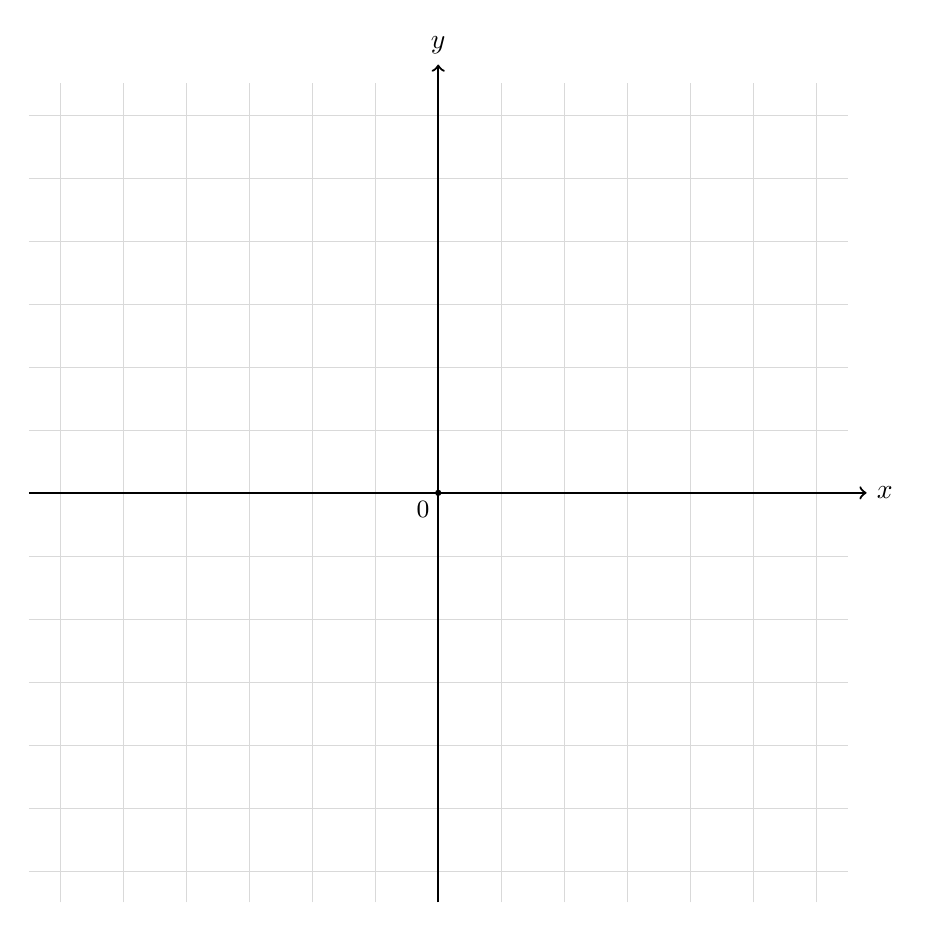
\begin{tikzpicture}[scale=0.8]
        % grid
        \draw[step=1cm,gray!30,very thin] (-6.5,-6.5) grid (6.5,6.5);
        % axes
        \draw[->,thick] (-6.5,0) -- (6.8,0) node[right] {$x$};
        \draw[->,thick] (0,-6.5) -- (0,6.8) node[above] {$y$};
        % origin
        \fill (0,0) circle (0.05) node[below left=2pt,fill=white,inner sep=1pt] {\small $0$};
    \end{tikzpicture}
    \end{center}
\end{enumerate}
\FloatBarrier

% Exercício 29: MAT_P4FUNCOE_4FIN_ANA_001.bak_agent_20251127T121826Z.tex
% Exercise ID: MAT_P4FUNCOE_4FIN_ANA_001
% Module: MÓDULO P4 - Funções | Concept: Função Inversa | Type: Determinação Analítica
% Difficulty: 2/5 (Fácil) | Type: desenvolvimento
% Points: 10 | Time: 10 min
% Tags: inversa, funcao_linear, grafico, expressao_analitica
% Author: Professor | Date: 2025-11-18
% Status: active
% Description: Determinar expressão analítica e representar graficamente função e inversa

\exercicio
Considere a função $f(x) = 2x - 3$.

\begin{enumerate}[label=\alph*]
    \item Determine a expressão analítica da função inversa $f^{-1}(x)$.
    
    \vspace{3cm}
    \item Represente graficamente a função $f$ e a sua inversa $f^{-1}$ no mesmo referencial.
    
    \vspace{3cm}

    \begin{center}
    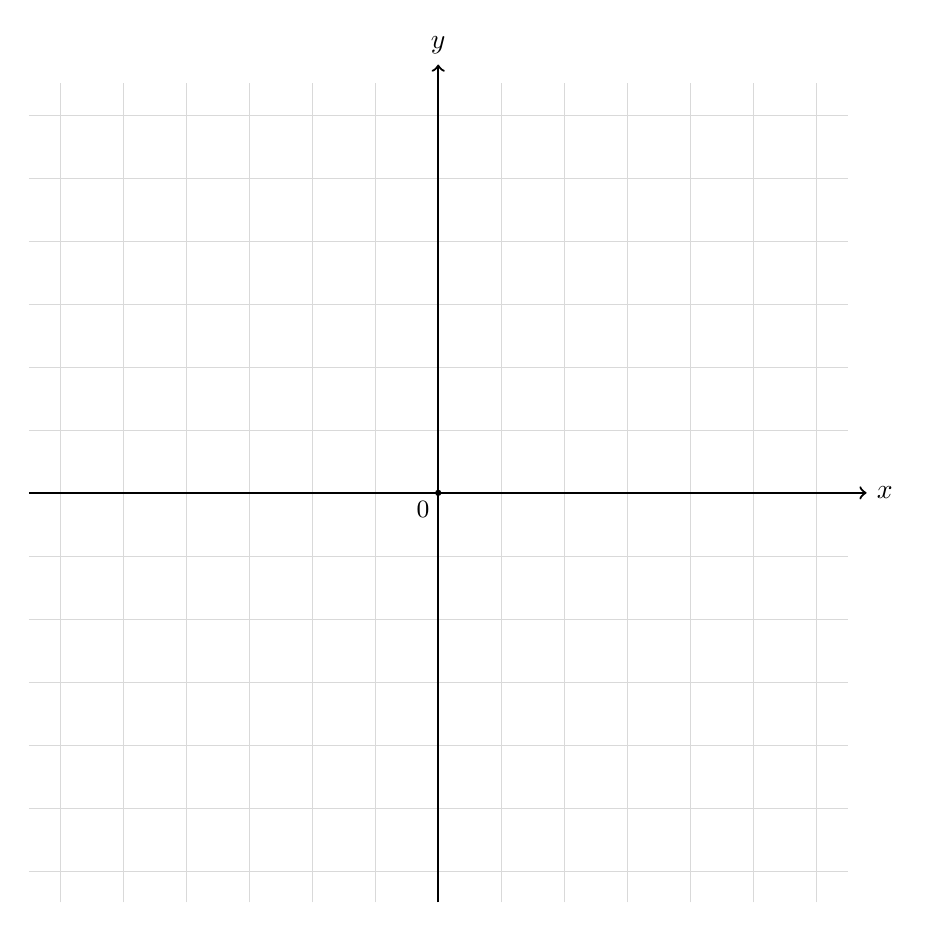
\begin{tikzpicture}[scale=0.8]
        % grid
        \draw[step=1cm,gray!30,very thin] (-6.5,-6.5) grid (6.5,6.5);
        % axes
        \draw[->,thick] (-6.5,0) -- (6.8,0) node[right] {$x$};
        \draw[->,thick] (0,-6.5) -- (0,6.8) node[above] {$y$};
        % origin
        \fill (0,0) circle (0.05) node[below left=2pt,fill=white,inner sep=1pt] {\small $0$};
    \end{tikzpicture}
    \end{center}
\end{enumerate}
\FloatBarrier

% Exercício 30: MAT_P4FUNCOE_4FIN_ANA_001.tex
% Exercise ID: MAT_P4FUNCOE_4FIN_ANA_001
% Module: MÓDULO P4 - Funções | Concept: Função Inversa | Type: Determinação Analítica
% Difficulty: 2/5 (Fácil) | Type: desenvolvimento
% Points: 10 | Time: 10 min
% Tags: inversa, funcao_linear, grafico, expressao_analitica
% Author: Professor | Date: 2025-11-18
% Status: active
% Description: Determinar expressão analítica e representar graficamente função e inversa

\exercicio
Considere a função $f(x) = 2x - 3$.

\begin{enumerate}[label=\alph*]
    \item Determine a expressão analítica da função inversa $f^{-1}(x)$.
    
    \vspace{3cm}
    \item Represente graficamente a função $f$ e a sua inversa $f^{-1}$ no mesmo referencial.
    
    \vspace{3cm}

    \begin{center}
    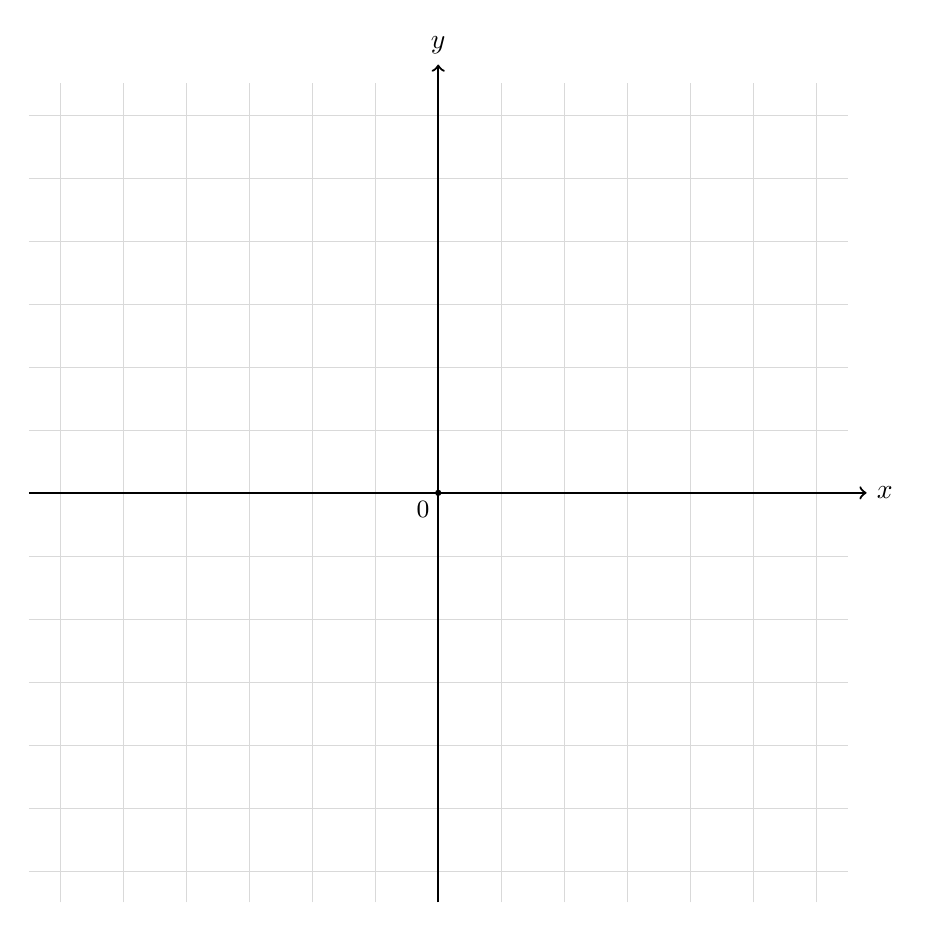
\begin{tikzpicture}[scale=0.8]
        % grid
        \draw[step=1cm,gray!30,very thin] (-6.5,-6.5) grid (6.5,6.5);
        % axes
        \draw[->,thick] (-6.5,0) -- (6.8,0) node[right] {$x$};
        \draw[->,thick] (0,-6.5) -- (0,6.8) node[above] {$y$};
        % origin
        \fill (0,0) circle (0.05) node[below left=2pt,fill=white,inner sep=1pt] {\small $0$};
    \end{tikzpicture}
    \end{center}
\end{enumerate}
\FloatBarrier

% Exercício 31: MAT_P4FUNCOE_4FIN_ANA_002.agentfix.tex
% Exercise ID: MAT_P4FUNCOE_4FIN_ANA_002
% Module: MÓDULO P4 - Funções | Concept: Função Inversa | Type: Determinação Analítica
% Difficulty: 2/5 (Fácil) | Type: desenvolvimento
% Points: 10 | Time: 10 min
% Tags: inversa, expressao_analitica, calculo
% Author: Professor | Date: 2025-11-18
% Status: active
% Description: Calcular a expressão da inversa de funções simples

\exercicio
Considere a função $f(x) = x - 1$.

\begin{enumerate}[label=\alph*]
    \item Determine a expressão analítica da função inversa $f^{-1}(x)$.
    
    \vspace{3cm}
    \item Represente graficamente a função $f$ e a sua inversa $f^{-1}$ no mesmo referencial.

        \begin{center}
    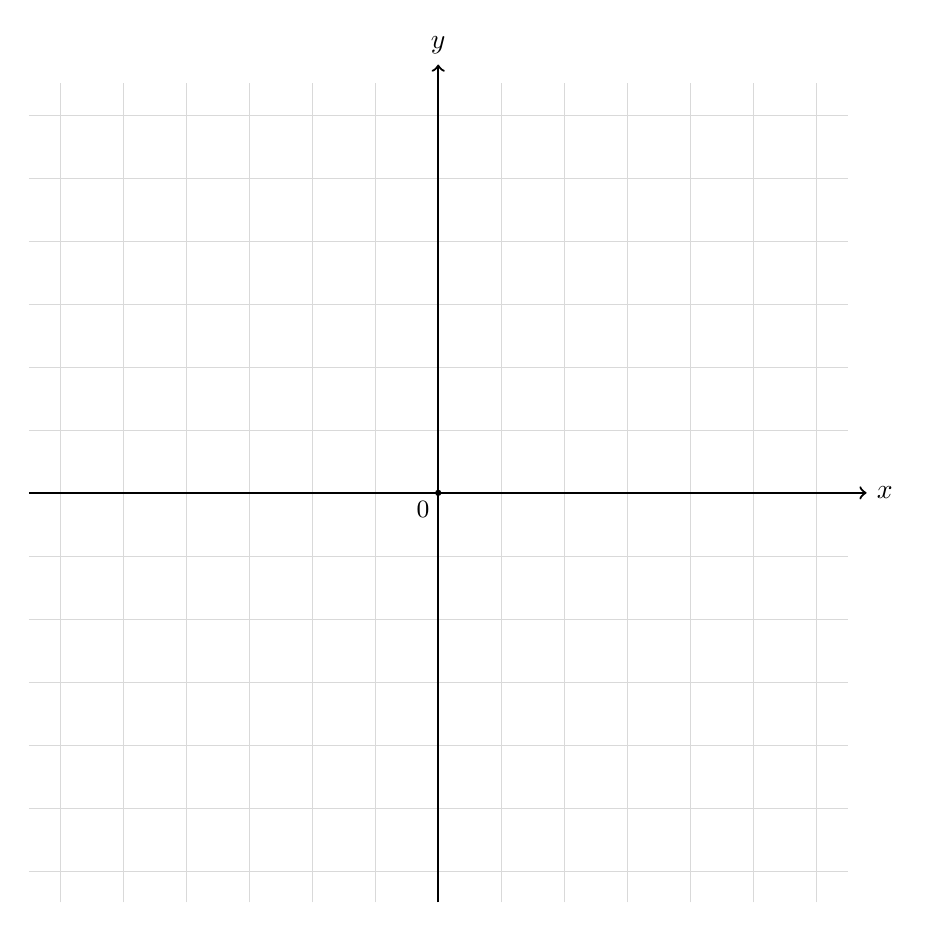
\begin{tikzpicture}[scale=0.8]
        % grid
        \draw[step=1cm,gray!30,very thin] (-6.5,-6.5) grid (6.5,6.5);
        % axes
        \draw[->,thick] (-6.5,0) -- (6.8,0) node[right] {$x$};
        \draw[->,thick] (0,-6.5) -- (0,6.8) node[above] {$y$};
        % origin
        \fill (0,0) circle (0.05) node[below left=2pt,fill=white,inner sep=1pt] {\small $0$};
    \end{tikzpicture}
    \end{center}

\end{enumerate}
\FloatBarrier

% Exercício 32: MAT_P4FUNCOE_4FIN_ANA_002.bak_agent_20251127T121826Z.tex
% Exercise ID: MAT_P4FUNCOE_4FIN_ANA_002
% Module: MÓDULO P4 - Funções | Concept: Função Inversa | Type: Determinação Analítica
% Difficulty: 2/5 (Fácil) | Type: desenvolvimento
% Points: 10 | Time: 10 min
% Tags: inversa, expressao_analitica, calculo
% Author: Professor | Date: 2025-11-18
% Status: active
% Description: Calcular a expressão da inversa de funções simples

\exercicio
Considere a função $f(x) = x - 1$.

\begin{enumerate}[label=\alph*]
    \item Determine a expressão analítica da função inversa $f^{-1}(x)$.
    
    \vspace{3cm}
    \item Represente graficamente a função $f$ e a sua inversa $f^{-1}$ no mesmo referencial.

        \begin{center}
    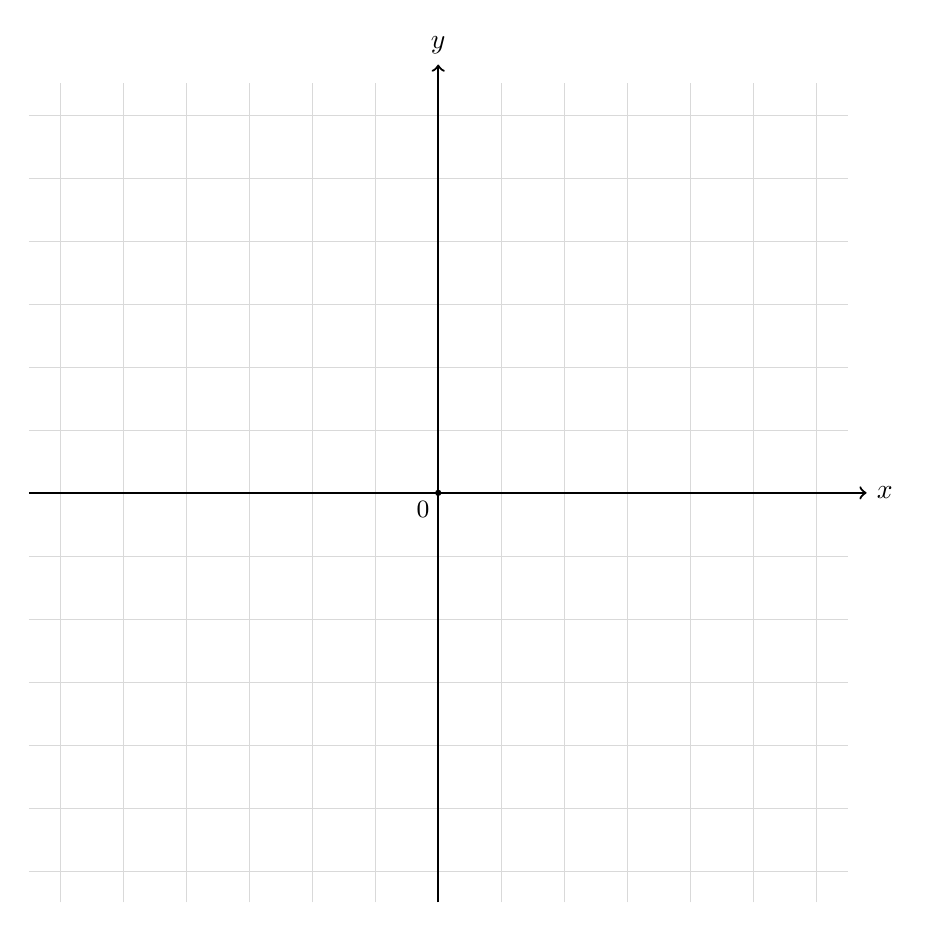
\begin{tikzpicture}[scale=0.8]
        % grid
        \draw[step=1cm,gray!30,very thin] (-6.5,-6.5) grid (6.5,6.5);
        % axes
        \draw[->,thick] (-6.5,0) -- (6.8,0) node[right] {$x$};
        \draw[->,thick] (0,-6.5) -- (0,6.8) node[above] {$y$};
        % origin
        \fill (0,0) circle (0.05) node[below left=2pt,fill=white,inner sep=1pt] {\small $0$};
    \end{tikzpicture}
    \end{center}

\end{enumerate}
\FloatBarrier

% Exercício 33: MAT_P4FUNCOE_4FIN_ANA_002.tex
% Exercise ID: MAT_P4FUNCOE_4FIN_ANA_002
% Module: MÓDULO P4 - Funções | Concept: Função Inversa | Type: Determinação Analítica
% Difficulty: 2/5 (Fácil) | Type: desenvolvimento
% Points: 10 | Time: 10 min
% Tags: inversa, expressao_analitica, calculo
% Author: Professor | Date: 2025-11-18
% Status: active
% Description: Calcular a expressão da inversa de funções simples

\exercicio
Considere a função $f(x) = x - 1$.

\begin{enumerate}[label=\alph*]
    \item Determine a expressão analítica da função inversa $f^{-1}(x)$.
    
    \vspace{3cm}
    \item Represente graficamente a função $f$ e a sua inversa $f^{-1}$ no mesmo referencial.

        \begin{center}
    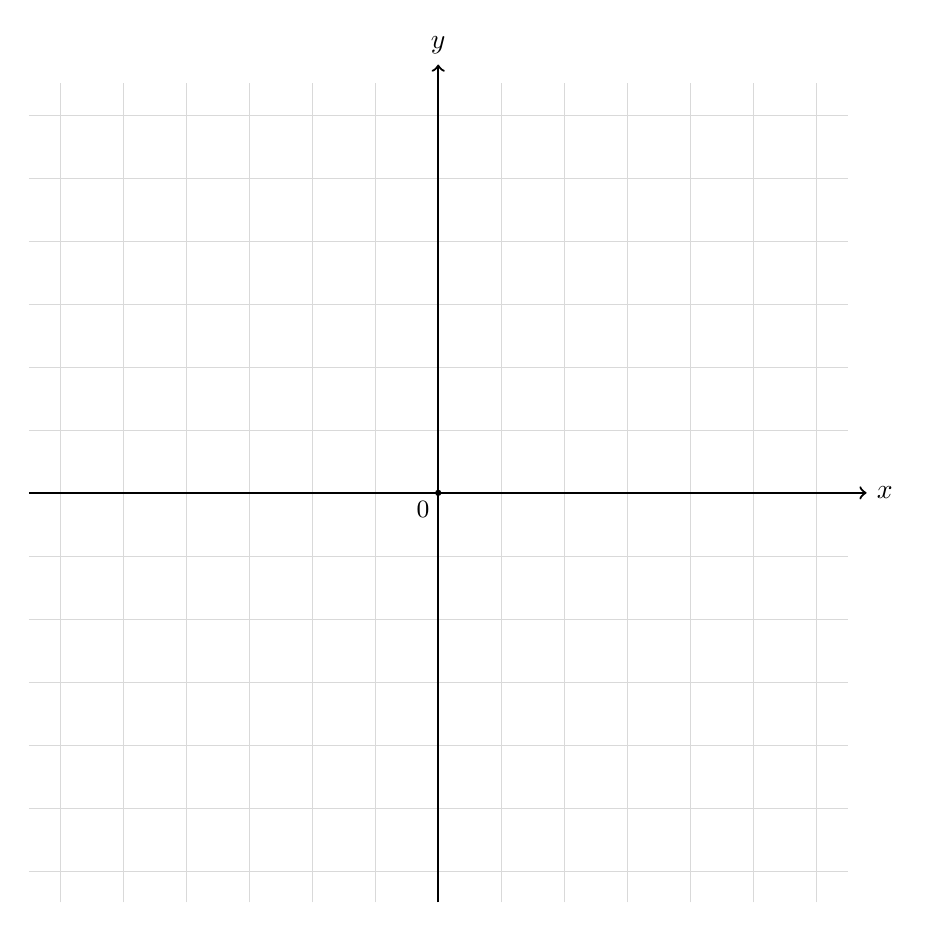
\begin{tikzpicture}[scale=0.8]
        % grid
        \draw[step=1cm,gray!30,very thin] (-6.5,-6.5) grid (6.5,6.5);
        % axes
        \draw[->,thick] (-6.5,0) -- (6.8,0) node[right] {$x$};
        \draw[->,thick] (0,-6.5) -- (0,6.8) node[above] {$y$};
        % origin
        \fill (0,0) circle (0.05) node[below left=2pt,fill=white,inner sep=1pt] {\small $0$};
    \end{tikzpicture}
    \end{center}

\end{enumerate}
\FloatBarrier

% Exercício 34: MAT_P4FUNCOE_4FIN_ANA_003.agentfix.tex
% Exercise ID: MAT_P4FUNCOE_4FIN_005
% Exercise ID: MAT_P4FUNCOE_4FIN_ANA_003
% Module: MÓDULO P4 - Funções | Concept: Função Inversa | Type: Determinação Analítica
% Difficulty: 2/5 (Fácil) | Type: desenvolvimento
% Points: 10 | Time: 10 min
% Tags: inversa, funcao_linear, grafico, expressao_analitica
% Author: Professor | Date: 2025-11-18
% Status: active
% Description: Determinar expressão analítica e representar graficamente função e inversa

\exercicio
Considere a função $f(x) = 2x - 4$.

\begin{enumerate}[label=\alph*]
    \item Determine a expressão analítica da função inversa $f^{-1}(x)$.
    
    \vspace{3cm}
    \item Represente graficamente a função $f$ e a sua inversa $f^{-1}$ no mesmo referencial.

        \begin{center}
    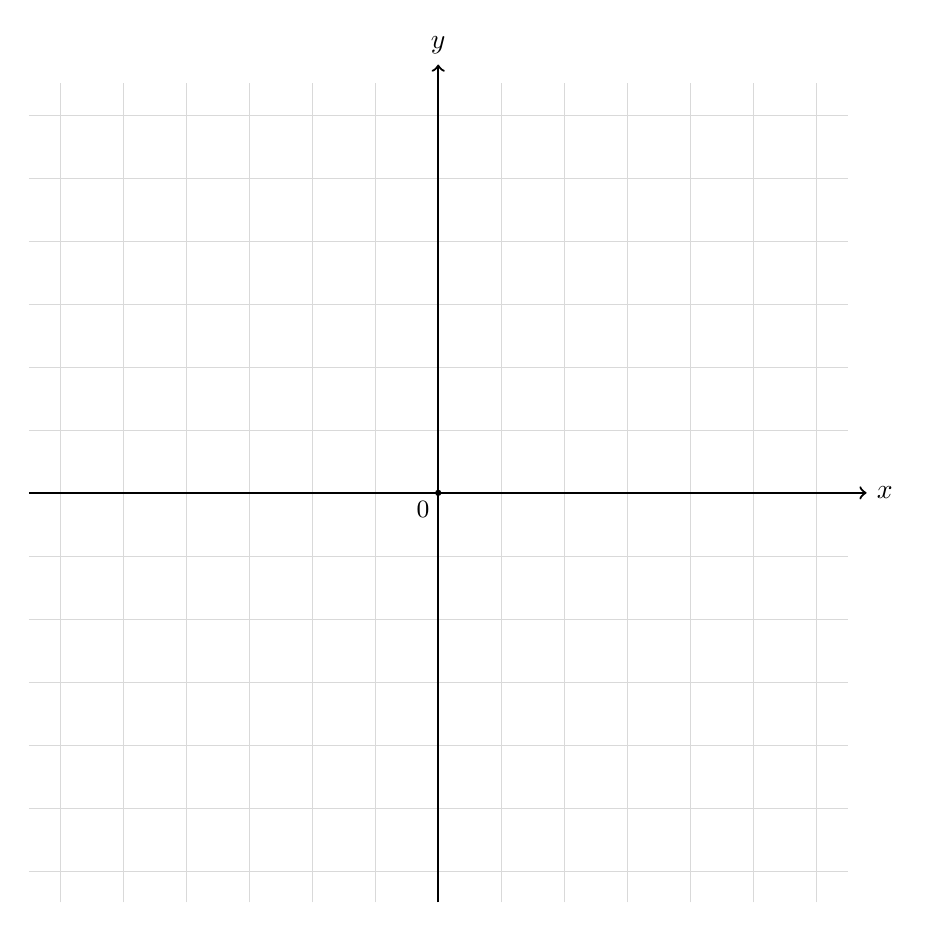
\begin{tikzpicture}[scale=0.8]
        % grid
        \draw[step=1cm,gray!30,very thin] (-6.5,-6.5) grid (6.5,6.5);
        % axes
        \draw[->,thick] (-6.5,0) -- (6.8,0) node[right] {$x$};
        \draw[->,thick] (0,-6.5) -- (0,6.8) node[above] {$y$};
        % origin
        \fill (0,0) circle (0.05) node[below left=2pt,fill=white,inner sep=1pt] {\small $0$};
    \end{tikzpicture}
    \end{center}

\end{enumerate}
\FloatBarrier

% Exercício 35: MAT_P4FUNCOE_4FIN_ANA_003.bak_agent_20251127T121826Z.tex
% Exercise ID: MAT_P4FUNCOE_4FIN_005
% Exercise ID: MAT_P4FUNCOE_4FIN_ANA_003
% Module: MÓDULO P4 - Funções | Concept: Função Inversa | Type: Determinação Analítica
% Difficulty: 2/5 (Fácil) | Type: desenvolvimento
% Points: 10 | Time: 10 min
% Tags: inversa, funcao_linear, grafico, expressao_analitica
% Author: Professor | Date: 2025-11-18
% Status: active
% Description: Determinar expressão analítica e representar graficamente função e inversa

\exercicio
Considere a função $f(x) = 2x - 4$.

\begin{enumerate}[label=\alph*]
    \item Determine a expressão analítica da função inversa $f^{-1}(x)$.
    
    \vspace{3cm}
    \item Represente graficamente a função $f$ e a sua inversa $f^{-1}$ no mesmo referencial.

        \begin{center}
    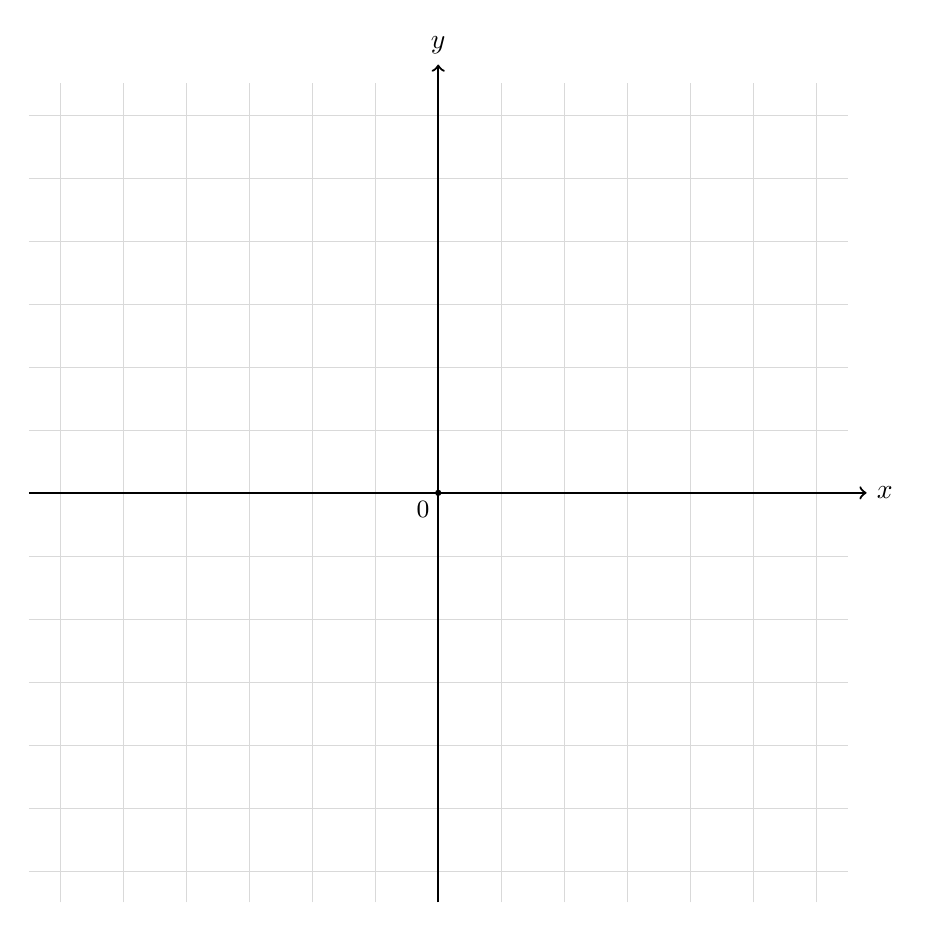
\begin{tikzpicture}[scale=0.8]
        % grid
        \draw[step=1cm,gray!30,very thin] (-6.5,-6.5) grid (6.5,6.5);
        % axes
        \draw[->,thick] (-6.5,0) -- (6.8,0) node[right] {$x$};
        \draw[->,thick] (0,-6.5) -- (0,6.8) node[above] {$y$};
        % origin
        \fill (0,0) circle (0.05) node[below left=2pt,fill=white,inner sep=1pt] {\small $0$};
    \end{tikzpicture}
    \end{center}

\end{enumerate}
\FloatBarrier

% Exercício 36: MAT_P4FUNCOE_4FIN_ANA_003.tex
% Exercise ID: MAT_P4FUNCOE_4FIN_005
% Exercise ID: MAT_P4FUNCOE_4FIN_ANA_003
% Module: MÓDULO P4 - Funções | Concept: Função Inversa | Type: Determinação Analítica
% Difficulty: 2/5 (Fácil) | Type: desenvolvimento
% Points: 10 | Time: 10 min
% Tags: inversa, funcao_linear, grafico, expressao_analitica
% Author: Professor | Date: 2025-11-18
% Status: active
% Description: Determinar expressão analítica e representar graficamente função e inversa

\exercicio
Considere a função $f(x) = 2x - 4$.

\begin{enumerate}[label=\alph*]
    \item Determine a expressão analítica da função inversa $f^{-1}(x)$.
    
    \vspace{3cm}
    \item Represente graficamente a função $f$ e a sua inversa $f^{-1}$ no mesmo referencial.

        \begin{center}
    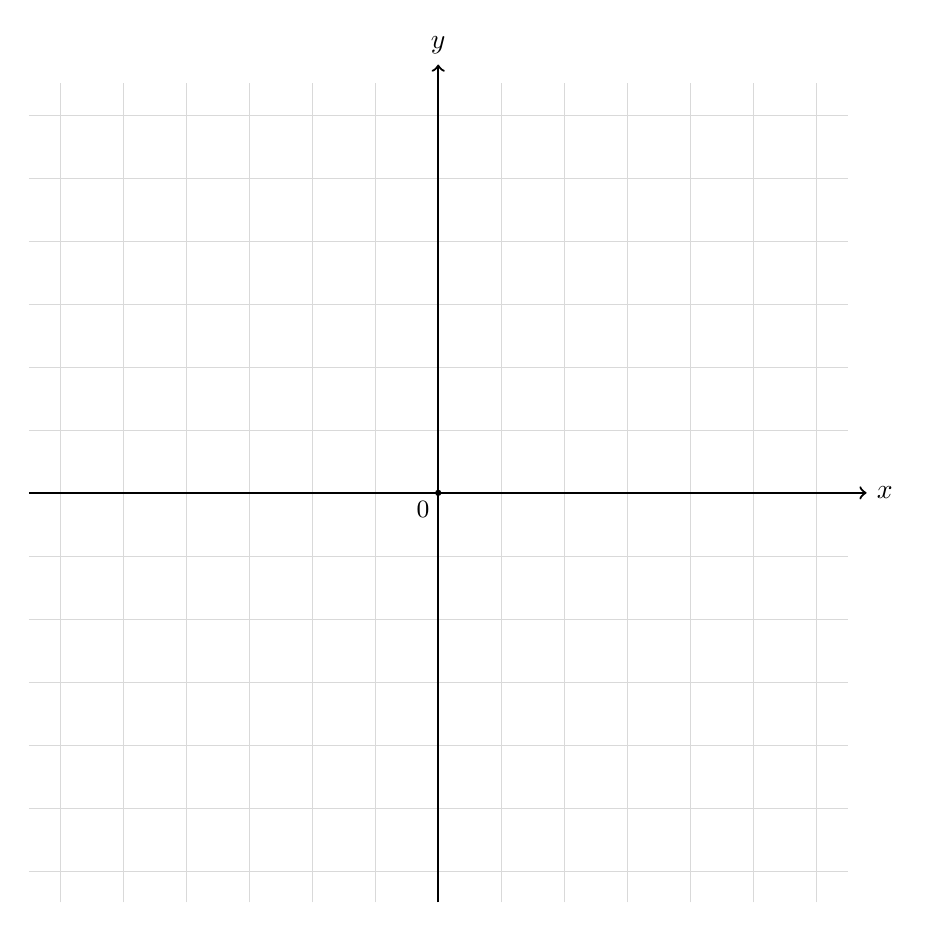
\begin{tikzpicture}[scale=0.8]
        % grid
        \draw[step=1cm,gray!30,very thin] (-6.5,-6.5) grid (6.5,6.5);
        % axes
        \draw[->,thick] (-6.5,0) -- (6.8,0) node[right] {$x$};
        \draw[->,thick] (0,-6.5) -- (0,6.8) node[above] {$y$};
        % origin
        \fill (0,0) circle (0.05) node[below left=2pt,fill=white,inner sep=1pt] {\small $0$};
    \end{tikzpicture}
    \end{center}

\end{enumerate}
\FloatBarrier

% Exercício 37: MAT_P4FUNCOE_4FIN_ANA_004.agentfix.tex
% Exercise ID: MAT_P4FUNCOE_4FIN_ANA_004
% Exercise ID: MAT_P4FUNCOE_4FIN_ANA_004
% Module: MÓDULO P4 - Funções | Concept: Função Inversa | Type: Determinação Analítica
% Difficulty: 2/5 (Fácil) | Type: desenvolvimento
% Points: 10 | Time: 10 min
% Tags: inversa, funcao_linear, grafico, expressao_analitica
% Author: Professor | Date: 2025-11-18
% Status: active
% Description: Determinar expressão analítica e representar graficamente função e inversa

\exercicio
Considere a função $f(x) = 3x - 1$.

\begin{enumerate}[label=\alph*]
    \item Determine a expressão analítica da função inversa $f^{-1}(x)$.
    
    \vspace{3cm}
    \item Represente graficamente a função $f$ e a sua inversa $f^{-1}$ no mesmo referencial.
    
    \vspace{3cm}

    \begin{center}
    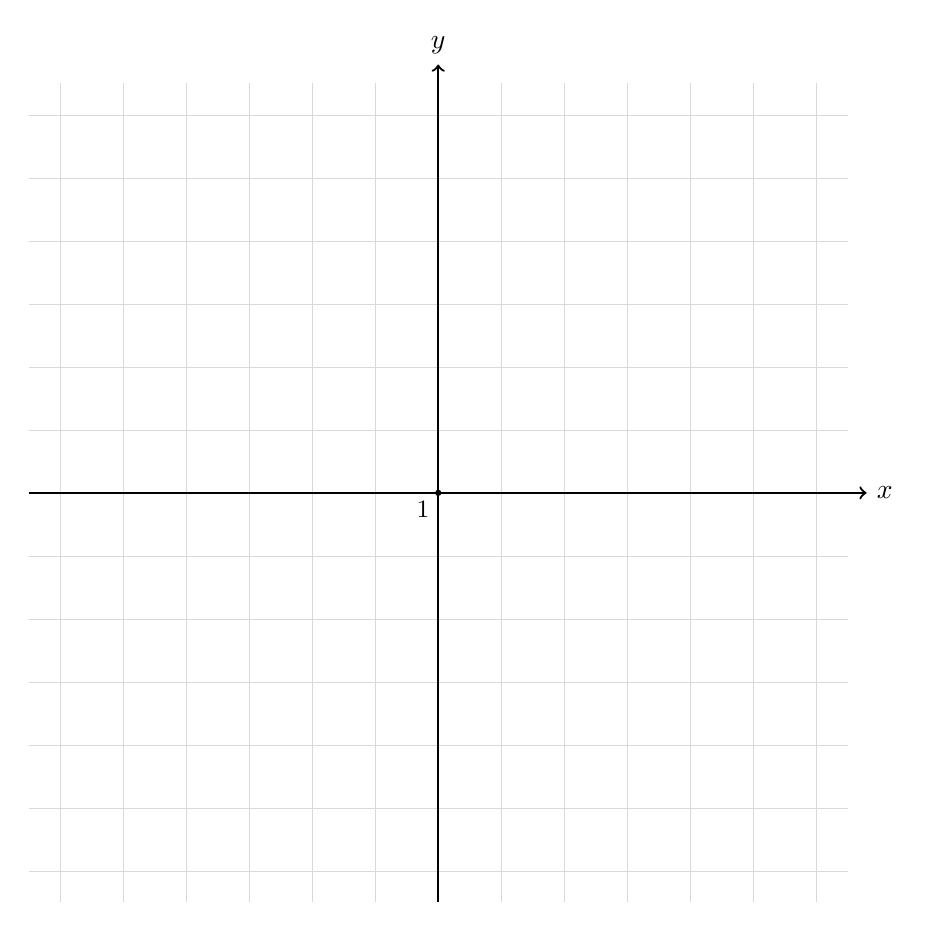
\begin{tikzpicture}[scale=0.8]
        % grid
        \draw[step=1cm,gray!30,very thin] (-6.5,-6.5) grid (6.5,6.5);
        % axes
        \draw[->,thick] (-6.5,0) -- (6.8,0) node[right] {$x$};
        \draw[->,thick] (0,-6.5) -- (0,6.8) node[above] {$y$};
        % origin
        \fill (0,0) circle (0.05) node[below left=2pt,fill=white,inner sep=1pt] {\small $1$};
    \end{tikzpicture}
    \end{center}
\end{enumerate}
\FloatBarrier

% Exercício 38: MAT_P4FUNCOE_4FIN_ANA_004.bak_agent_20251127T121826Z.tex
% Exercise ID: MAT_P4FUNCOE_4FIN_ANA_004
% Exercise ID: MAT_P4FUNCOE_4FIN_ANA_004
% Module: MÓDULO P4 - Funções | Concept: Função Inversa | Type: Determinação Analítica
% Difficulty: 2/5 (Fácil) | Type: desenvolvimento
% Points: 10 | Time: 10 min
% Tags: inversa, funcao_linear, grafico, expressao_analitica
% Author: Professor | Date: 2025-11-18
% Status: active
% Description: Determinar expressão analítica e representar graficamente função e inversa

\exercicio
Considere a função $f(x) = 3x - 1$.

\begin{enumerate}[label=\alph*]
    \item Determine a expressão analítica da função inversa $f^{-1}(x)$.
    
    \vspace{3cm}
    \item Represente graficamente a função $f$ e a sua inversa $f^{-1}$ no mesmo referencial.
    
    \vspace{3cm}

    \begin{center}
    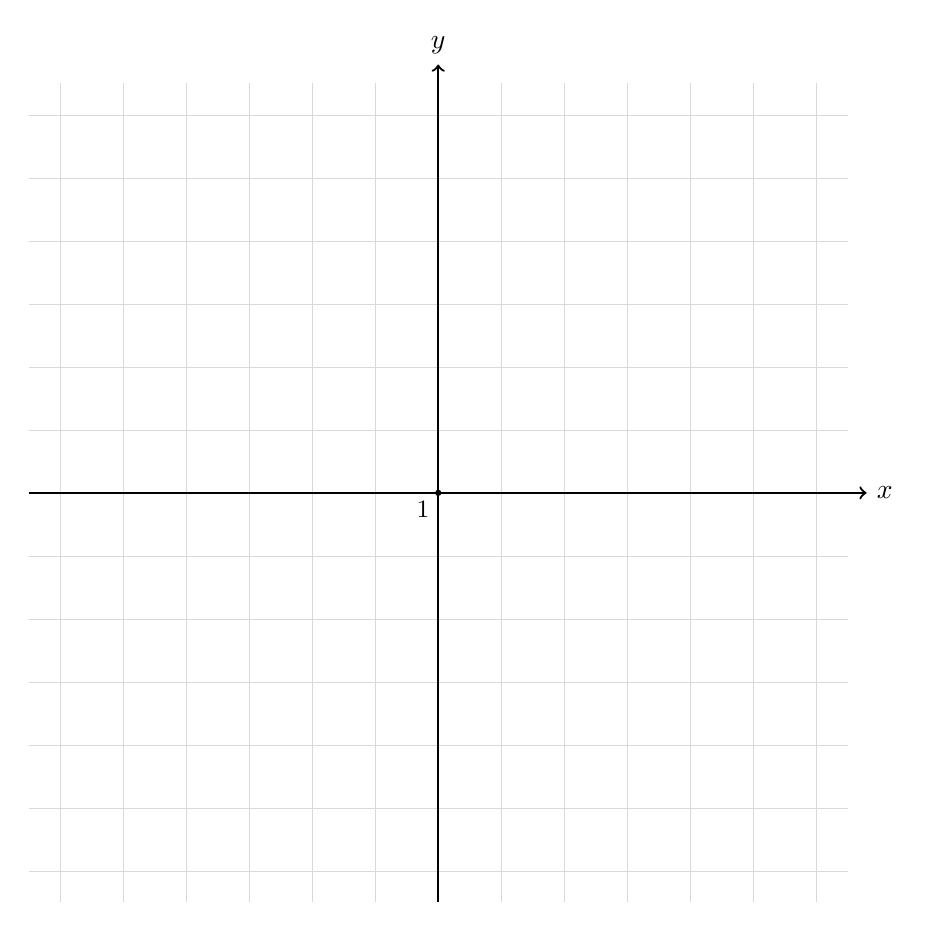
\begin{tikzpicture}[scale=0.8]
        % grid
        \draw[step=1cm,gray!30,very thin] (-6.5,-6.5) grid (6.5,6.5);
        % axes
        \draw[->,thick] (-6.5,0) -- (6.8,0) node[right] {$x$};
        \draw[->,thick] (0,-6.5) -- (0,6.8) node[above] {$y$};
        % origin
        \fill (0,0) circle (0.05) node[below left=2pt,fill=white,inner sep=1pt] {\small $1$};
    \end{tikzpicture}
    \end{center}
\end{enumerate}
\FloatBarrier

% Exercício 39: MAT_P4FUNCOE_4FIN_ANA_004.tex
% Exercise ID: MAT_P4FUNCOE_4FIN_ANA_004
% Exercise ID: MAT_P4FUNCOE_4FIN_ANA_004
% Module: MÓDULO P4 - Funções | Concept: Função Inversa | Type: Determinação Analítica
% Difficulty: 2/5 (Fácil) | Type: desenvolvimento
% Points: 10 | Time: 10 min
% Tags: inversa, funcao_linear, grafico, expressao_analitica
% Author: Professor | Date: 2025-11-18
% Status: active
% Description: Determinar expressão analítica e representar graficamente função e inversa

\exercicio
Considere a função $f(x) = 3x - 1$.

\begin{enumerate}[label=\alph*]
    \item Determine a expressão analítica da função inversa $f^{-1}(x)$.
    
    \vspace{3cm}
    \item Represente graficamente a função $f$ e a sua inversa $f^{-1}$ no mesmo referencial.
    
    \vspace{3cm}

    \begin{center}
    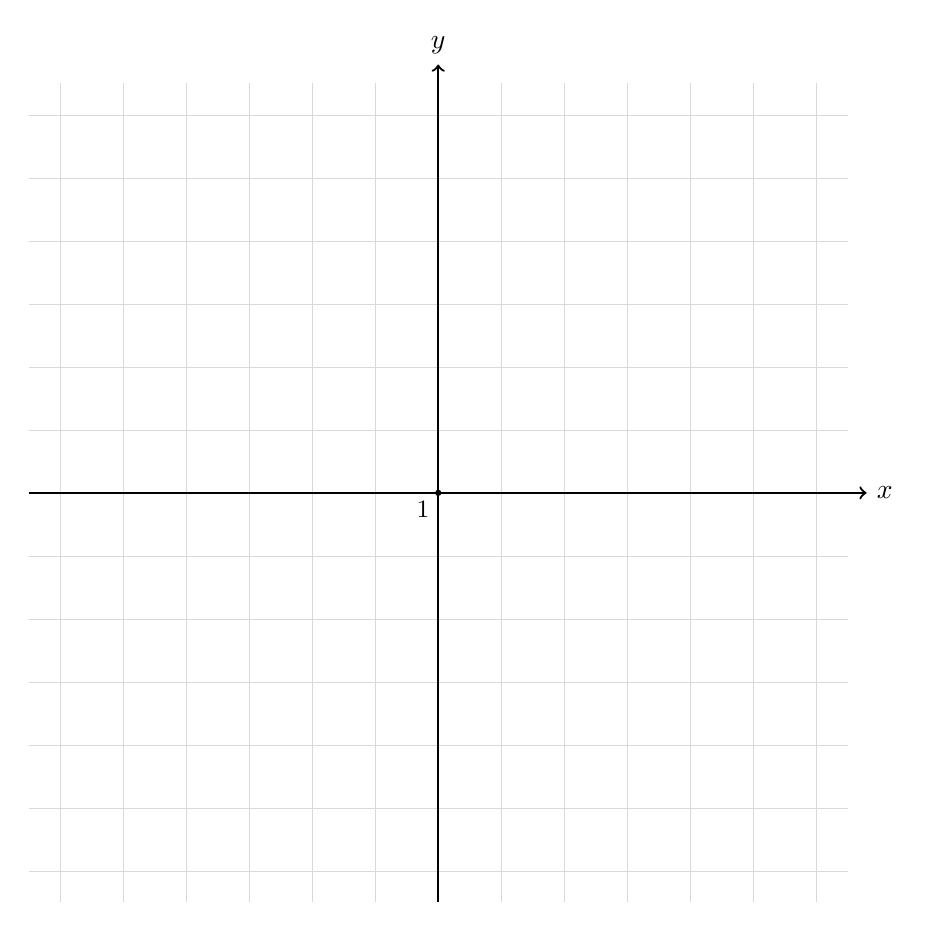
\begin{tikzpicture}[scale=0.8]
        % grid
        \draw[step=1cm,gray!30,very thin] (-6.5,-6.5) grid (6.5,6.5);
        % axes
        \draw[->,thick] (-6.5,0) -- (6.8,0) node[right] {$x$};
        \draw[->,thick] (0,-6.5) -- (0,6.8) node[above] {$y$};
        % origin
        \fill (0,0) circle (0.05) node[below left=2pt,fill=white,inner sep=1pt] {\small $1$};
    \end{tikzpicture}
    \end{center}
\end{enumerate}
\FloatBarrier

% Exercício 40: MAT_P4FUNCOE_4FIN_ANA_005.agentfix.tex
% Exercise ID: MAT_P4FUNCOE_4FIN_ANA_005
% Exercise ID: MAT_P4FUNCOE_4FIN_ANA_005
% Module: MÓDULO P4 - Funções | Concept: Função Inversa | Type: Determinação Analítica
% Difficulty: 2/5 (Fácil) | Type: desenvolvimento
% Points: 10 | Time: 10 min
% Tags: inversa, funcao_linear, grafico, expressao_analitica
% Author: Professor | Date: 2025-11-18
% Status: active
% Description: Determinar expressão analítica e representar graficamente função e inversa

\exercicio
Considere a função $f(x) = 4x - 1$.

\begin{enumerate}[label=\alph*]
    \item Determine a expressão analítica da função inversa $f^{-1}(x)$.
    
    \vspace{3cm}
    \item Represente graficamente a função $f$ e a sua inversa $f^{-1}$ no mesmo referencial.
    
    \vspace{3cm}

    \begin{center}
    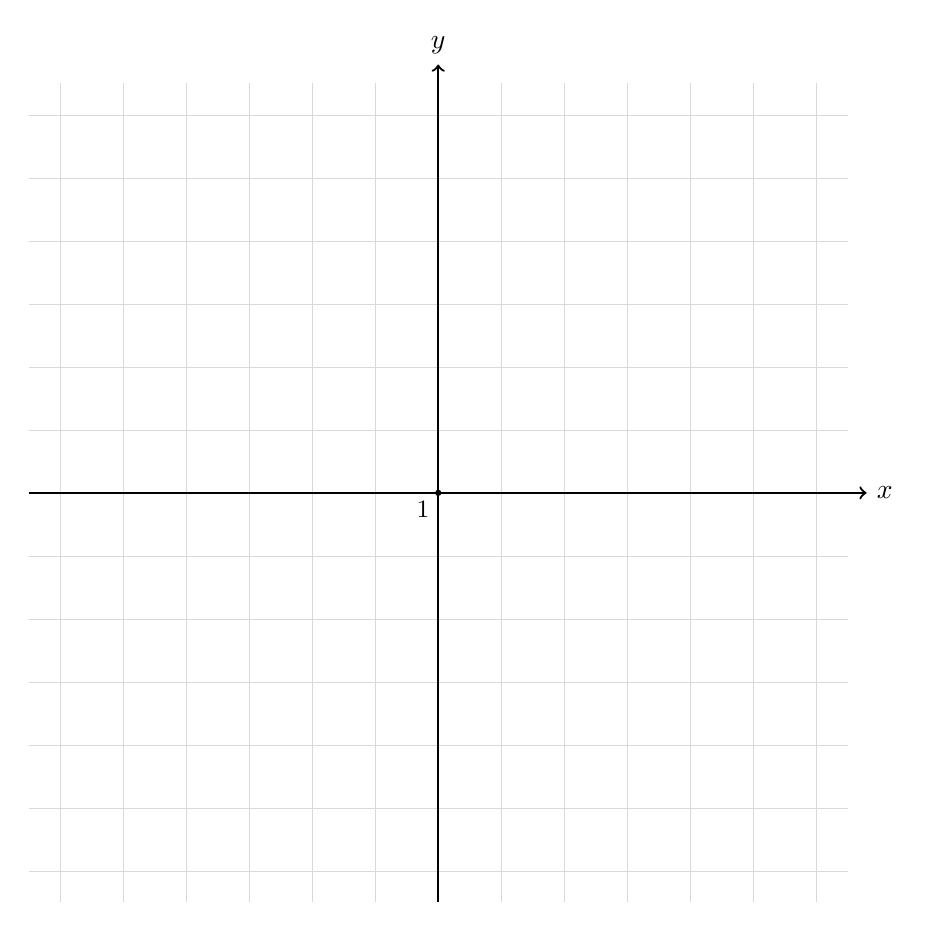
\begin{tikzpicture}[scale=0.8]
        % grid
        \draw[step=1cm,gray!30,very thin] (-6.5,-6.5) grid (6.5,6.5);
        % axes
        \draw[->,thick] (-6.5,0) -- (6.8,0) node[right] {$x$};
        \draw[->,thick] (0,-6.5) -- (0,6.8) node[above] {$y$};
        % origin
        \fill (0,0) circle (0.05) node[below left=2pt,fill=white,inner sep=1pt] {\small $1$};
    \end{tikzpicture}
    \end{center}
\end{enumerate}
\FloatBarrier

% Exercício 41: MAT_P4FUNCOE_4FIN_ANA_005.bak_agent_20251127T121826Z.tex
% Exercise ID: MAT_P4FUNCOE_4FIN_ANA_005
% Exercise ID: MAT_P4FUNCOE_4FIN_ANA_005
% Module: MÓDULO P4 - Funções | Concept: Função Inversa | Type: Determinação Analítica
% Difficulty: 2/5 (Fácil) | Type: desenvolvimento
% Points: 10 | Time: 10 min
% Tags: inversa, funcao_linear, grafico, expressao_analitica
% Author: Professor | Date: 2025-11-18
% Status: active
% Description: Determinar expressão analítica e representar graficamente função e inversa

\exercicio
Considere a função $f(x) = 4x - 1$.

\begin{enumerate}[label=\alph*]
    \item Determine a expressão analítica da função inversa $f^{-1}(x)$.
    
    \vspace{3cm}
    \item Represente graficamente a função $f$ e a sua inversa $f^{-1}$ no mesmo referencial.
    
    \vspace{3cm}

    \begin{center}
    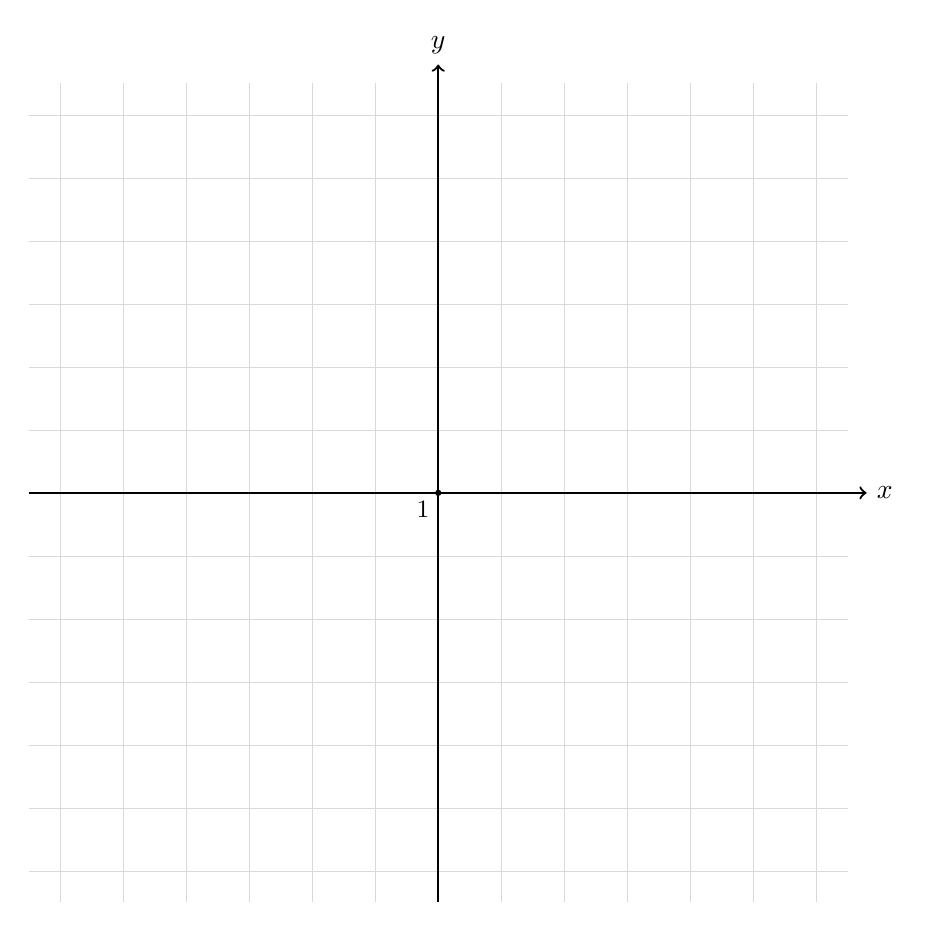
\begin{tikzpicture}[scale=0.8]
        % grid
        \draw[step=1cm,gray!30,very thin] (-6.5,-6.5) grid (6.5,6.5);
        % axes
        \draw[->,thick] (-6.5,0) -- (6.8,0) node[right] {$x$};
        \draw[->,thick] (0,-6.5) -- (0,6.8) node[above] {$y$};
        % origin
        \fill (0,0) circle (0.05) node[below left=2pt,fill=white,inner sep=1pt] {\small $1$};
    \end{tikzpicture}
    \end{center}
\end{enumerate}
\FloatBarrier

% Exercício 42: MAT_P4FUNCOE_4FIN_ANA_005.tex
% Exercise ID: MAT_P4FUNCOE_4FIN_ANA_005
% Exercise ID: MAT_P4FUNCOE_4FIN_ANA_005
% Module: MÓDULO P4 - Funções | Concept: Função Inversa | Type: Determinação Analítica
% Difficulty: 2/5 (Fácil) | Type: desenvolvimento
% Points: 10 | Time: 10 min
% Tags: inversa, funcao_linear, grafico, expressao_analitica
% Author: Professor | Date: 2025-11-18
% Status: active
% Description: Determinar expressão analítica e representar graficamente função e inversa

\exercicio
Considere a função $f(x) = 4x - 1$.

\begin{enumerate}[label=\alph*]
    \item Determine a expressão analítica da função inversa $f^{-1}(x)$.
    
    \vspace{3cm}
    \item Represente graficamente a função $f$ e a sua inversa $f^{-1}$ no mesmo referencial.
    
    \vspace{3cm}

    \begin{center}
    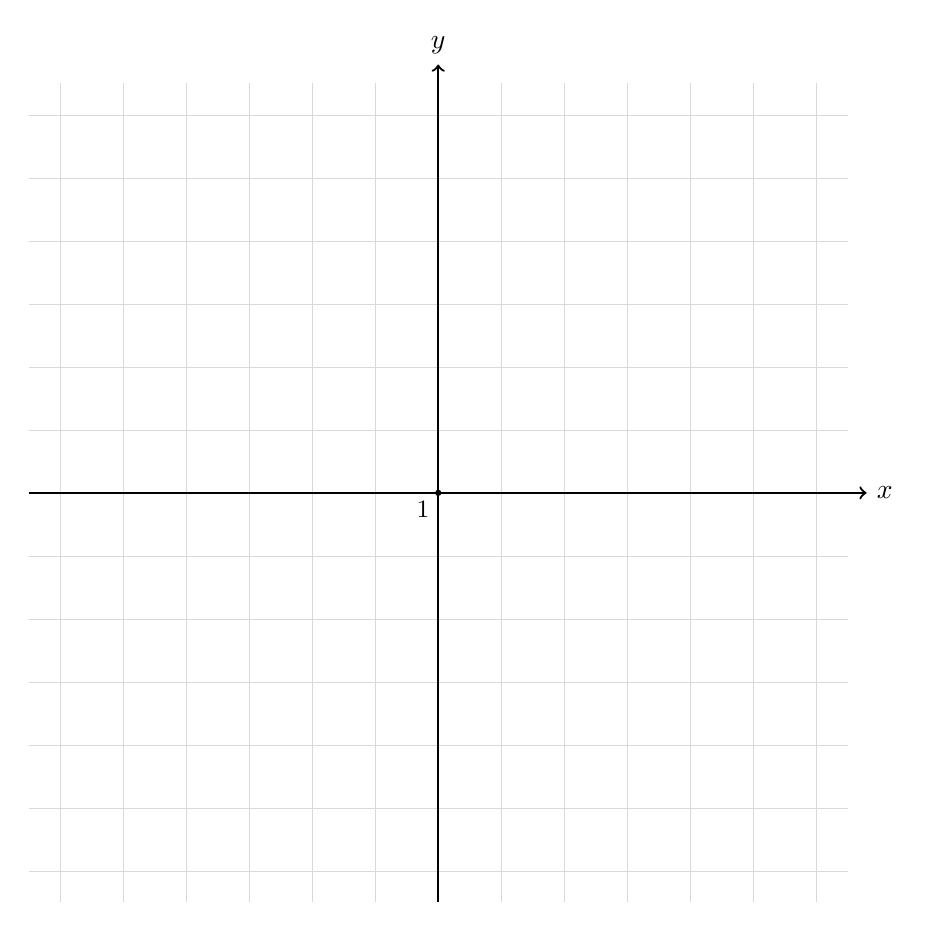
\begin{tikzpicture}[scale=0.8]
        % grid
        \draw[step=1cm,gray!30,very thin] (-6.5,-6.5) grid (6.5,6.5);
        % axes
        \draw[->,thick] (-6.5,0) -- (6.8,0) node[right] {$x$};
        \draw[->,thick] (0,-6.5) -- (0,6.8) node[above] {$y$};
        % origin
        \fill (0,0) circle (0.05) node[below left=2pt,fill=white,inner sep=1pt] {\small $1$};
    \end{tikzpicture}
    \end{center}
\end{enumerate}
\FloatBarrier

% Exercício 43: MAT_P4FUNCOE_4FIN_ANA_006.agentfix.tex
% Exercise ID: MAT_P4FUNCOE_4FIN_ANA_006
% Exercise ID: MAT_P4FUNCOE_4FIN_ANA_006
% Module: MÓDULO P4 - Funções | Concept: Função Inversa | Type: Determinação Analítica
% Difficulty: 2/5 (Fácil) | Type: desenvolvimento
% Points: 10 | Time: 10 min
% Tags: inversa, expressao_analitica, calculo
% Author: Professor | Date: 2025-11-18
% Status: active
% Description: Calcular a expressão da inversa de funções simples

\exercicio
Considere a função $g(x)=2x$.

\begin{enumerate}[label=\alph*]
    \item Determine a expressão analítica da função inversa $g^{-1}(x)$.
    
    \vspace{3cm}
    \item Represente graficamente a função $g$ e a sua inversa $g^{-1}$ no mesmo referencial.
    
    \begin{center}
    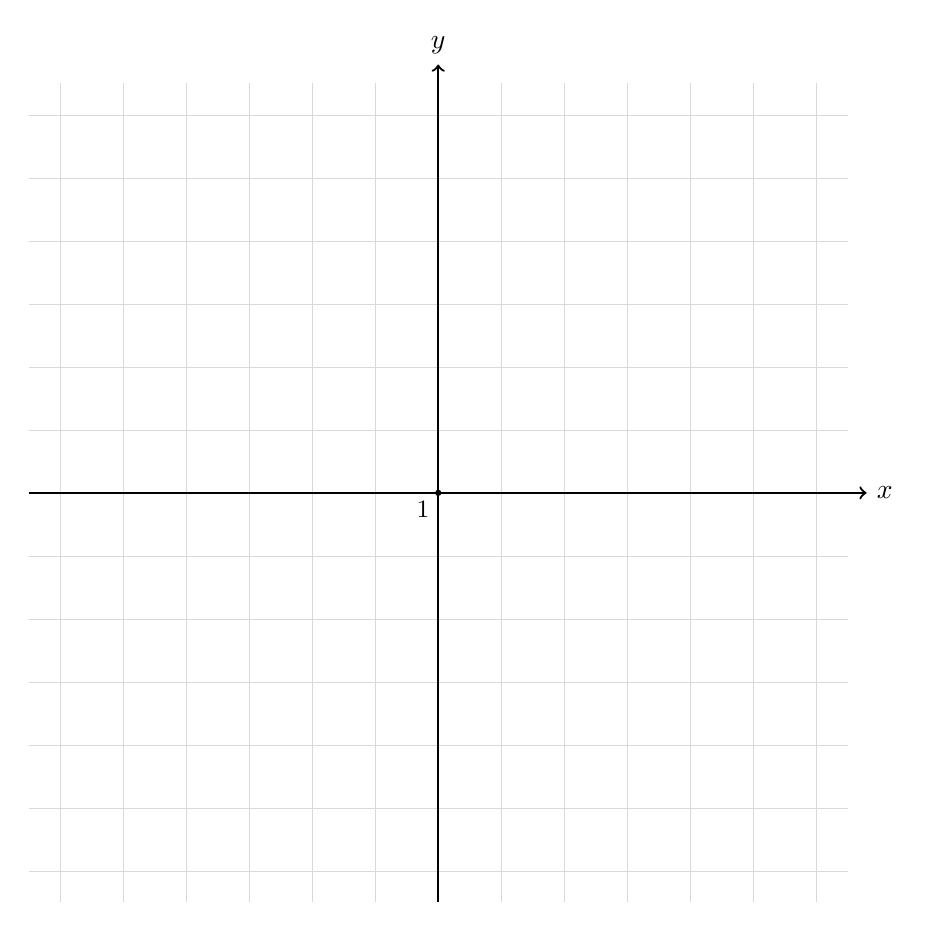
\begin{tikzpicture}[scale=0.8]
        % grid
        \draw[step=1cm,gray!30,very thin] (-6.5,-6.5) grid (6.5,6.5);
        % axes
        \draw[->,thick] (-6.5,0) -- (6.8,0) node[right] {$x$};
        \draw[->,thick] (0,-6.5) -- (0,6.8) node[above] {$y$};
        % origin
        \fill (0,0) circle (0.05) node[below left=2pt,fill=white,inner sep=1pt] {\small $1$};
    \end{tikzpicture}
    \end{center}

\end{enumerate}
\FloatBarrier

% Exercício 44: MAT_P4FUNCOE_4FIN_ANA_006.bak_agent_20251127T121826Z.tex
% Exercise ID: MAT_P4FUNCOE_4FIN_ANA_006
% Exercise ID: MAT_P4FUNCOE_4FIN_ANA_006
% Module: MÓDULO P4 - Funções | Concept: Função Inversa | Type: Determinação Analítica
% Difficulty: 2/5 (Fácil) | Type: desenvolvimento
% Points: 10 | Time: 10 min
% Tags: inversa, expressao_analitica, calculo
% Author: Professor | Date: 2025-11-18
% Status: active
% Description: Calcular a expressão da inversa de funções simples

\exercicio
Considere a função $g(x)=2x$.

\begin{enumerate}[label=\alph*]
    \item Determine a expressão analítica da função inversa $g^{-1}(x)$.
    
    \vspace{3cm}
    \item Represente graficamente a função $g$ e a sua inversa $g^{-1}$ no mesmo referencial.
    
    \begin{center}
    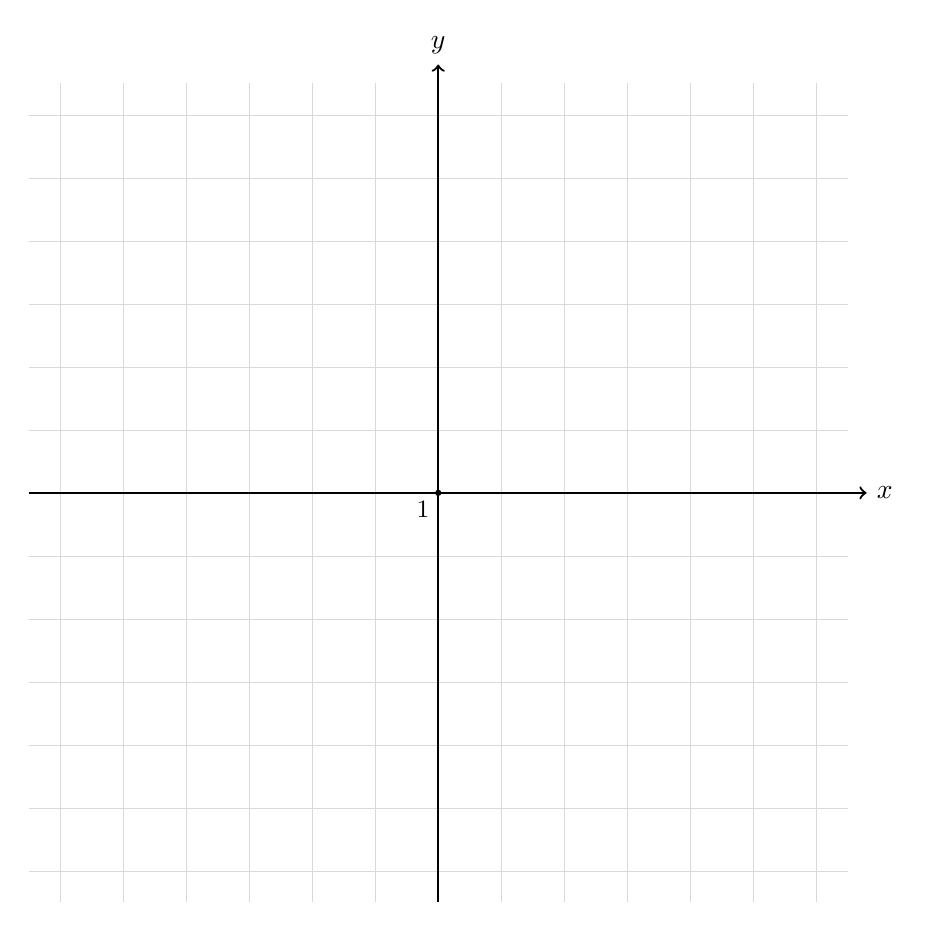
\begin{tikzpicture}[scale=0.8]
        % grid
        \draw[step=1cm,gray!30,very thin] (-6.5,-6.5) grid (6.5,6.5);
        % axes
        \draw[->,thick] (-6.5,0) -- (6.8,0) node[right] {$x$};
        \draw[->,thick] (0,-6.5) -- (0,6.8) node[above] {$y$};
        % origin
        \fill (0,0) circle (0.05) node[below left=2pt,fill=white,inner sep=1pt] {\small $1$};
    \end{tikzpicture}
    \end{center}

\end{enumerate}
\FloatBarrier

% Exercício 45: MAT_P4FUNCOE_4FIN_ANA_006.tex
% Exercise ID: MAT_P4FUNCOE_4FIN_ANA_006
% Exercise ID: MAT_P4FUNCOE_4FIN_ANA_006
% Module: MÓDULO P4 - Funções | Concept: Função Inversa | Type: Determinação Analítica
% Difficulty: 2/5 (Fácil) | Type: desenvolvimento
% Points: 10 | Time: 10 min
% Tags: inversa, expressao_analitica, calculo
% Author: Professor | Date: 2025-11-18
% Status: active
% Description: Calcular a expressão da inversa de funções simples

\exercicio
Considere a função $g(x)=2x$.

\begin{enumerate}[label=\alph*]
    \item Determine a expressão analítica da função inversa $g^{-1}(x)$.
    
    \vspace{3cm}
    \item Represente graficamente a função $g$ e a sua inversa $g^{-1}$ no mesmo referencial.
    
    \begin{center}
    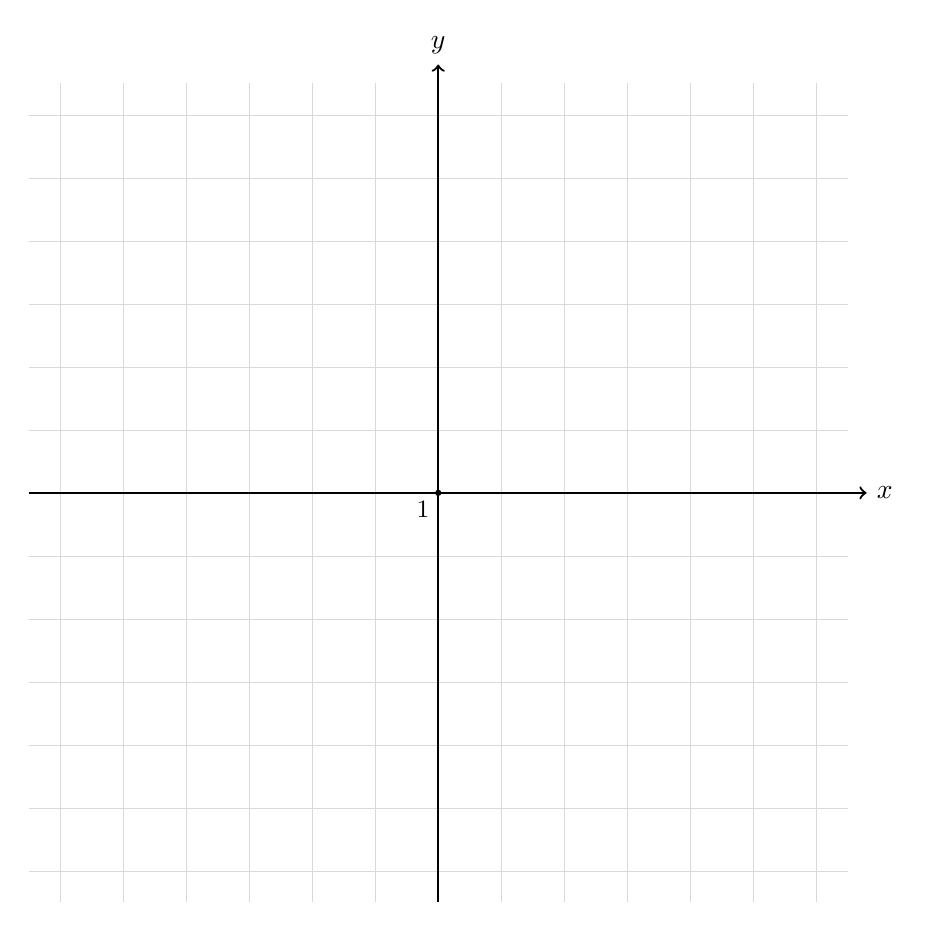
\begin{tikzpicture}[scale=0.8]
        % grid
        \draw[step=1cm,gray!30,very thin] (-6.5,-6.5) grid (6.5,6.5);
        % axes
        \draw[->,thick] (-6.5,0) -- (6.8,0) node[right] {$x$};
        \draw[->,thick] (0,-6.5) -- (0,6.8) node[above] {$y$};
        % origin
        \fill (0,0) circle (0.05) node[below left=2pt,fill=white,inner sep=1pt] {\small $1$};
    \end{tikzpicture}
    \end{center}

\end{enumerate}
\FloatBarrier

% Exercício 46: MAT_P4FUNCOE_4FIN_GRA_001.agentfix.tex
% Exercise ID: MAT_P4FUNCOE_4FIN_GRA_001
% Module: MÓDULO P4 - Funções | Concept: Função Inversa | Type: Determinação Gráfica
% Difficulty: 2/5 (Fácil) | Type: desenvolvimento
% Points: 10 | Time: 10 min
% Tags: inversa, grafico, simetria, funcao_quadratica
% Author: Professor | Date: 2025-11-18
% Status: active
% Description: Dado o gráfico de ramos de funções, desenhar o gráfico da inversa

\exercicio
Na figura está representado o gráfico de uma função $f$ definida em $[0, +\infty[$. Represente, no referencial dado, o gráfico da função inversa $f^{-1}$.

\begin{figure}[ht]
\centering
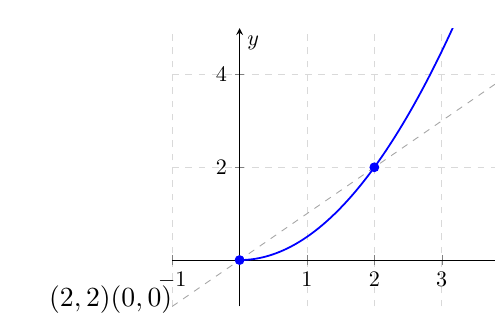
\begin{tikzpicture}[scale=0.8]
    \begin{axis}[
        axis lines = middle,
        xlabel = $x$,
        ylabel = $y$,
        xmin = -1, xmax = 5,
        ymin = -1, ymax = 5,
        grid = major,
        grid style = {dashed, gray!30},
        width = 8cm,
        height = 6cm,
    ]
    \addplot[domain=-1:5, dashed, gray!70, thin] {x};
    
    \addplot[domain=0:4, samples=100, thick, blue] {x^2/2};
    \addplot[mark=*, mark size=2pt, blue] coordinates {(0,0)};
    \addplot[mark=*, mark size=2pt, blue] coordinates {(2,2)};
    
ode[anchor=south west] at (axis cs:2,2.2) {$(2,2)$};
    
ode[anchor=north east] at (axis cs:0.2,0.2) {$(0,0)$};
    \end{axis}
\end{tikzpicture}
\end{figure}

\bigskip

\exercicio
Na figura está representado o gráfico de uma função $g$. Represente, no referencial dado, o gráfico da função inversa $g^{-1}$.

\begin{figure}[H]
\centering
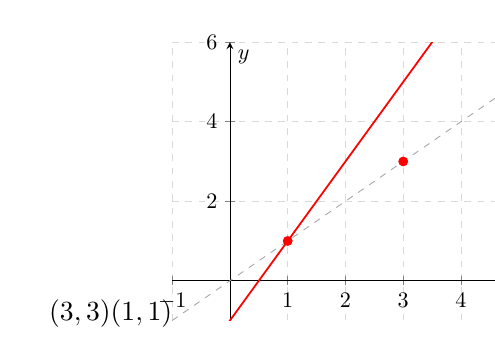
\begin{tikzpicture}[scale=0.8]
    \begin{axis}[
        axis lines = middle,
        xlabel = $x$,
        ylabel = $y$,
        xmin = -1, xmax = 6,
        ymin = -1, ymax = 6,
        grid = major,
        grid style = {dashed, gray!30},
        width = 8cm,
        height = 6cm,
    ]
    \addplot[domain=-1:6, dashed, gray!70, thin] {x};
    
    \addplot[domain=-1:5, thick, red] {2*x-1};
    \addplot[mark=*, mark size=2pt, red] coordinates {(1,1)};
    \addplot[mark=*, mark size=2pt, red] coordinates {(3,3)};
    
ode[anchor=south west] at (axis cs:3,3.2) {$(3,3)$};
    
ode[anchor=north east] at (axis cs:1.15,1.1) {$(1,1)$};
    \end{axis}
\end{tikzpicture}
\end{figure}
\vspace{3cm}
}
\FloatBarrier

% Exercício 47: MAT_P4FUNCOE_4FIN_GRA_001.bak_agent_20251127T121826Z.tex
% Exercise ID: MAT_P4FUNCOE_4FIN_GRA_001
% Module: MÓDULO P4 - Funções | Concept: Função Inversa | Type: Determinação Gráfica
% Difficulty: 2/5 (Fácil) | Type: desenvolvimento
% Points: 10 | Time: 10 min
% Tags: inversa, grafico, simetria, funcao_quadratica
% Author: Professor | Date: 2025-11-18
% Status: active
% Description: Dado o gráfico de ramos de funções, desenhar o gráfico da inversa

\exercicio
Na figura está representado o gráfico de uma função $f$ definida em $[0, +\infty[$. Represente, no referencial dado, o gráfico da função inversa $f^{-1}$.

\begin{figure}[ht]
\centering
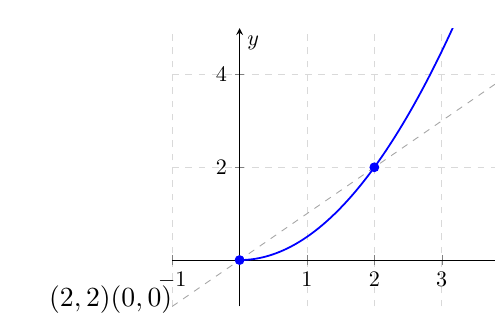
\begin{tikzpicture}[scale=0.8]
    \begin{axis}[
        axis lines = middle,
        xlabel = $x$,
        ylabel = $y$,
        xmin = -1, xmax = 5,
        ymin = -1, ymax = 5,
        grid = major,
        grid style = {dashed, gray!30},
        width = 8cm,
        height = 6cm,
    ]
    \addplot[domain=-1:5, dashed, gray!70, thin] {x};
    
    \addplot[domain=0:4, samples=100, thick, blue] {x^2/2};
    \addplot[mark=*, mark size=2pt, blue] coordinates {(0,0)};
    \addplot[mark=*, mark size=2pt, blue] coordinates {(2,2)};
    
ode[anchor=south west] at (axis cs:2,2.2) {$(2,2)$};
    
ode[anchor=north east] at (axis cs:0.2,0.2) {$(0,0)$};
    \end{axis}
\end{tikzpicture}
\end{figure}

\bigskip

\exercicio
Na figura está representado o gráfico de uma função $g$. Represente, no referencial dado, o gráfico da função inversa $g^{-1}$.

\begin{figure}[H]
\centering
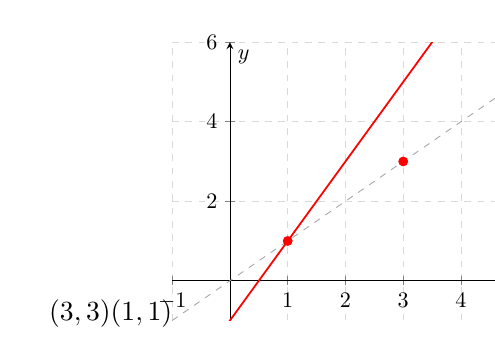
\begin{tikzpicture}[scale=0.8]
    \begin{axis}[
        axis lines = middle,
        xlabel = $x$,
        ylabel = $y$,
        xmin = -1, xmax = 6,
        ymin = -1, ymax = 6,
        grid = major,
        grid style = {dashed, gray!30},
        width = 8cm,
        height = 6cm,
    ]
    \addplot[domain=-1:6, dashed, gray!70, thin] {x};
    
    \addplot[domain=-1:5, thick, red] {2*x-1};
    \addplot[mark=*, mark size=2pt, red] coordinates {(1,1)};
    \addplot[mark=*, mark size=2pt, red] coordinates {(3,3)};
    
ode[anchor=south west] at (axis cs:3,3.2) {$(3,3)$};
    
ode[anchor=north east] at (axis cs:1.15,1.1) {$(1,1)$};
    \end{axis}
\end{tikzpicture}
\end{figure
\vspace{3cm}
}
\FloatBarrier

% Exercício 48: MAT_P4FUNCOE_4FIN_GRA_001.tex
% Exercise ID: MAT_P4FUNCOE_4FIN_GRA_001
% Module: MÓDULO P4 - Funções | Concept: Função Inversa | Type: Determinação Gráfica
% Difficulty: 2/5 (Fácil) | Type: desenvolvimento
% Points: 10 | Time: 10 min
% Tags: inversa, grafico, simetria, funcao_quadratica
% Author: Professor | Date: 2025-11-18
% Status: active
% Description: Dado o gráfico de ramos de funções, desenhar o gráfico da inversa

\exercicio
Na figura está representado o gráfico de uma função $f$ definida em $[0, +\infty[$. Represente, no referencial dado, o gráfico da função inversa $f^{-1}$.

\begin{figure}[ht]
\centering
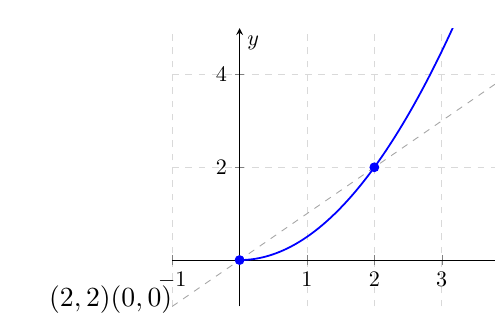
\begin{tikzpicture}[scale=0.8]
    \begin{axis}[
        axis lines = middle,
        xlabel = $x$,
        ylabel = $y$,
        xmin = -1, xmax = 5,
        ymin = -1, ymax = 5,
        grid = major,
        grid style = {dashed, gray!30},
        width = 8cm,
        height = 6cm,
    ]
    \addplot[domain=-1:5, dashed, gray!70, thin] {x};
    
    \addplot[domain=0:4, samples=100, thick, blue] {x^2/2};
    \addplot[mark=*, mark size=2pt, blue] coordinates {(0,0)};
    \addplot[mark=*, mark size=2pt, blue] coordinates {(2,2)};
    
ode[anchor=south west] at (axis cs:2,2.2) {$(2,2)$};
    
ode[anchor=north east] at (axis cs:0.2,0.2) {$(0,0)$};
    \end{axis}
\end{tikzpicture}
\end{figure}

\bigskip

\exercicio
Na figura está representado o gráfico de uma função $g$. Represente, no referencial dado, o gráfico da função inversa $g^{-1}$.

\begin{figure}[H]
\centering
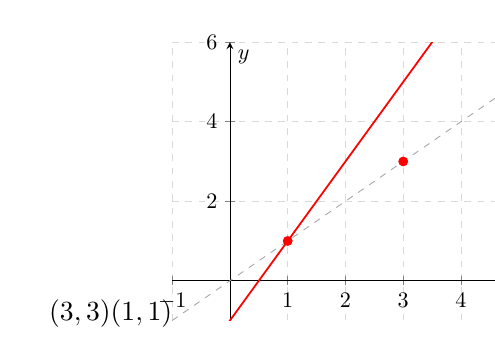
\begin{tikzpicture}[scale=0.8]
    \begin{axis}[
        axis lines = middle,
        xlabel = $x$,
        ylabel = $y$,
        xmin = -1, xmax = 6,
        ymin = -1, ymax = 6,
        grid = major,
        grid style = {dashed, gray!30},
        width = 8cm,
        height = 6cm,
    ]
    \addplot[domain=-1:6, dashed, gray!70, thin] {x};
    
    \addplot[domain=-1:5, thick, red] {2*x-1};
    \addplot[mark=*, mark size=2pt, red] coordinates {(1,1)};
    \addplot[mark=*, mark size=2pt, red] coordinates {(3,3)};
    
ode[anchor=south west] at (axis cs:3,3.2) {$(3,3)$};
    
ode[anchor=north east] at (axis cs:1.15,1.1) {$(1,1)$};
    \end{axis}
\end{tikzpicture}
\end{figure
\vspace{3cm}
}
\FloatBarrier

% Exercício 49: MAT_P4FUNCOE_4FIN_GRA_002.agentfix.tex
% Exercise ID: MAT_P4FUNCOE_4FIN_GRA_002
% Exercise ID: MAT_P4FUNCOE_4FIN_GRA_002
% Module: MÓDULO P4 - Funções | Concept: Função Inversa | Type: Determinação Gráfica
% Difficulty: 2/5 (Fácil) | Type: desenvolvimento
% Points: 10 | Time: 10 min
% Tags: inversa, grafico, simetria, funcao_quadratica
% Author: Professor | Date: 2025-11-18
% Status: active
% Description: Dado o gráfico de ramos de funções, desenhar o gráfico da inversa

\exercicio
Na figura está representado o gráfico de uma função $h$ definida em $]-\infty, 0]$. Represente, no referencial dado, o gráfico da função inversa $h^{-1}$.

\begin{figure}[ht]
\centering
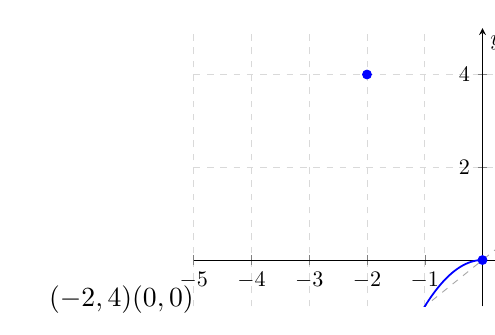
\begin{tikzpicture}[scale=0.8]
    \begin{axis}[
        axis lines = middle,
        xlabel = $x$,
        ylabel = $y$,
        xmin = -5, xmax = 2,
        ymin = -1, ymax = 5,
        grid = major,
        grid style = {dashed, gray!30},
        width = 8cm,
        height = 6cm,
    ]
    \addplot[domain=-5:5, dashed, gray!70, thin] {x};
    
    \addplot[domain=-4:0, samples=100, thick, blue] {-x^2};
    \addplot[mark=*, mark size=2pt, blue] coordinates {(0,0)};
    \addplot[mark=*, mark size=2pt, blue] coordinates {(-2,4)};
    
ode[anchor=east] at (axis cs:-2.2,4) {$(-2,4)$};
    
ode[anchor=north west] at (axis cs:0.2,0.2) {$(0,0)$};
    \end{axis}
\end{tikzpicture}
\end{figure}

\bigskip

\exercicio
Na figura está representado o gráfico de uma função $k$ definida em $[1, 5]$. Represente, no referencial dado, o gráfico da função inversa $k^{-1}$.

\begin{figure}[H]
\centering
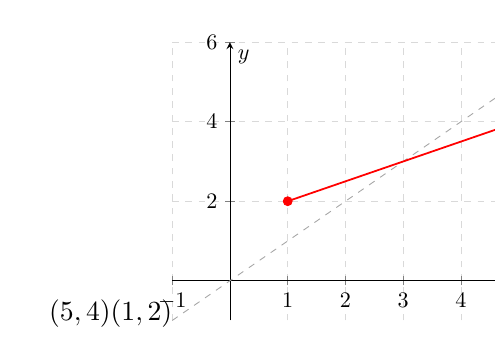
\begin{tikzpicture}[scale=0.8]
    \begin{axis}[
        axis lines = middle,
        xlabel = $x$,
        ylabel = $y$,
        xmin = -1, xmax = 6,
        ymin = -1, ymax = 6,
        grid = major,
        grid style = {dashed, gray!30},
        width = 8cm,
        height = 6cm,
    ]
    \addplot[domain=-1:6, dashed, gray!70, thin] {x};
    
    \addplot[domain=1:5, thick, red] {0.5*x+1.5};
    \addplot[mark=*, mark size=2pt, red] coordinates {(1,2)};
    \addplot[mark=*, mark size=2pt, red] coordinates {(5,4)};
    
ode[anchor=south west] at (axis cs:5,4.2) {$(5,4)$};
    
ode[anchor=north east] at (axis cs:1,1.8) {$(1,2)$};
    \end{axis}
\end{tikzpicture}
\end{figure}
\vspace{3cm}
}
\FloatBarrier

% Exercício 50: MAT_P4FUNCOE_4FIN_GRA_002.bak_agent_20251127T121826Z.tex
% Exercise ID: MAT_P4FUNCOE_4FIN_GRA_002
% Exercise ID: MAT_P4FUNCOE_4FIN_GRA_002
% Module: MÓDULO P4 - Funções | Concept: Função Inversa | Type: Determinação Gráfica
% Difficulty: 2/5 (Fácil) | Type: desenvolvimento
% Points: 10 | Time: 10 min
% Tags: inversa, grafico, simetria, funcao_quadratica
% Author: Professor | Date: 2025-11-18
% Status: active
% Description: Dado o gráfico de ramos de funções, desenhar o gráfico da inversa

\exercicio
Na figura está representado o gráfico de uma função $h$ definida em $]-\infty, 0]$. Represente, no referencial dado, o gráfico da função inversa $h^{-1}$.

\begin{figure}[ht]
\centering
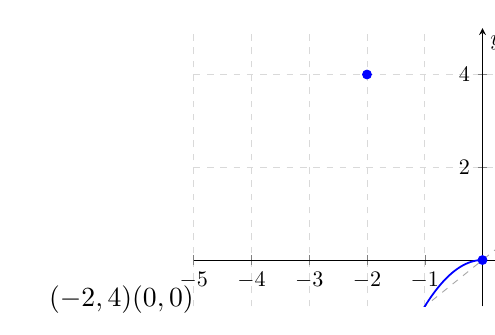
\begin{tikzpicture}[scale=0.8]
    \begin{axis}[
        axis lines = middle,
        xlabel = $x$,
        ylabel = $y$,
        xmin = -5, xmax = 2,
        ymin = -1, ymax = 5,
        grid = major,
        grid style = {dashed, gray!30},
        width = 8cm,
        height = 6cm,
    ]
    \addplot[domain=-5:5, dashed, gray!70, thin] {x};
    
    \addplot[domain=-4:0, samples=100, thick, blue] {-x^2};
    \addplot[mark=*, mark size=2pt, blue] coordinates {(0,0)};
    \addplot[mark=*, mark size=2pt, blue] coordinates {(-2,4)};
    
ode[anchor=east] at (axis cs:-2.2,4) {$(-2,4)$};
    
ode[anchor=north west] at (axis cs:0.2,0.2) {$(0,0)$};
    \end{axis}
\end{tikzpicture}
\end{figure}

\bigskip

\exercicio
Na figura está representado o gráfico de uma função $k$ definida em $[1, 5]$. Represente, no referencial dado, o gráfico da função inversa $k^{-1}$.

\begin{figure}[H]
\centering
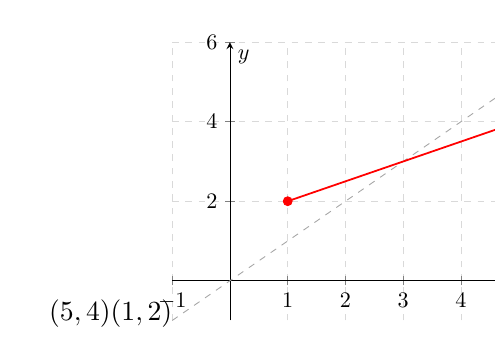
\begin{tikzpicture}[scale=0.8]
    \begin{axis}[
        axis lines = middle,
        xlabel = $x$,
        ylabel = $y$,
        xmin = -1, xmax = 6,
        ymin = -1, ymax = 6,
        grid = major,
        grid style = {dashed, gray!30},
        width = 8cm,
        height = 6cm,
    ]
    \addplot[domain=-1:6, dashed, gray!70, thin] {x};
    
    \addplot[domain=1:5, thick, red] {0.5*x+1.5};
    \addplot[mark=*, mark size=2pt, red] coordinates {(1,2)};
    \addplot[mark=*, mark size=2pt, red] coordinates {(5,4)};
    
ode[anchor=south west] at (axis cs:5,4.2) {$(5,4)$};
    
ode[anchor=north east] at (axis cs:1,1.8) {$(1,2)$};
    \end{axis}
\end{tikzpicture}
\end{figure
\vspace{3cm}
}
\FloatBarrier

% Exercício 51: MAT_P4FUNCOE_4FIN_GRA_002.tex
% Exercise ID: MAT_P4FUNCOE_4FIN_GRA_002
% Exercise ID: MAT_P4FUNCOE_4FIN_GRA_002
% Module: MÓDULO P4 - Funções | Concept: Função Inversa | Type: Determinação Gráfica
% Difficulty: 2/5 (Fácil) | Type: desenvolvimento
% Points: 10 | Time: 10 min
% Tags: inversa, grafico, simetria, funcao_quadratica
% Author: Professor | Date: 2025-11-18
% Status: active
% Description: Dado o gráfico de ramos de funções, desenhar o gráfico da inversa

\exercicio
Na figura está representado o gráfico de uma função $h$ definida em $]-\infty, 0]$. Represente, no referencial dado, o gráfico da função inversa $h^{-1}$.

\begin{figure}[ht]
\centering
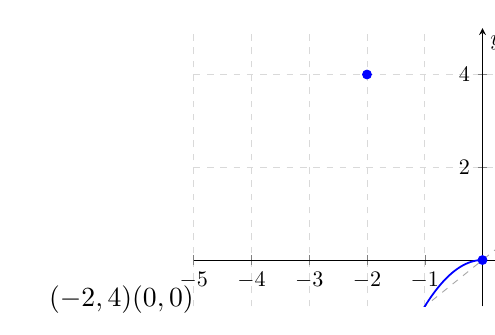
\begin{tikzpicture}[scale=0.8]
    \begin{axis}[
        axis lines = middle,
        xlabel = $x$,
        ylabel = $y$,
        xmin = -5, xmax = 2,
        ymin = -1, ymax = 5,
        grid = major,
        grid style = {dashed, gray!30},
        width = 8cm,
        height = 6cm,
    ]
    \addplot[domain=-5:5, dashed, gray!70, thin] {x};
    
    \addplot[domain=-4:0, samples=100, thick, blue] {-x^2};
    \addplot[mark=*, mark size=2pt, blue] coordinates {(0,0)};
    \addplot[mark=*, mark size=2pt, blue] coordinates {(-2,4)};
    
ode[anchor=east] at (axis cs:-2.2,4) {$(-2,4)$};
    
ode[anchor=north west] at (axis cs:0.2,0.2) {$(0,0)$};
    \end{axis}
\end{tikzpicture}
\end{figure}

\bigskip

\exercicio
Na figura está representado o gráfico de uma função $k$ definida em $[1, 5]$. Represente, no referencial dado, o gráfico da função inversa $k^{-1}$.

\begin{figure}[H]
\centering
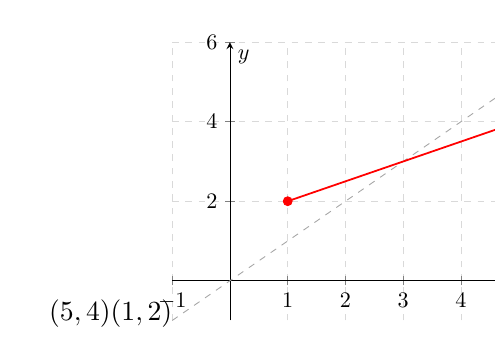
\begin{tikzpicture}[scale=0.8]
    \begin{axis}[
        axis lines = middle,
        xlabel = $x$,
        ylabel = $y$,
        xmin = -1, xmax = 6,
        ymin = -1, ymax = 6,
        grid = major,
        grid style = {dashed, gray!30},
        width = 8cm,
        height = 6cm,
    ]
    \addplot[domain=-1:6, dashed, gray!70, thin] {x};
    
    \addplot[domain=1:5, thick, red] {0.5*x+1.5};
    \addplot[mark=*, mark size=2pt, red] coordinates {(1,2)};
    \addplot[mark=*, mark size=2pt, red] coordinates {(5,4)};
    
ode[anchor=south west] at (axis cs:5,4.2) {$(5,4)$};
    
ode[anchor=north east] at (axis cs:1,1.8) {$(1,2)$};
    \end{axis}
\end{tikzpicture}
\end{figure
\vspace{3cm}
}
\FloatBarrier

% Exercício 52: MAT_P4FUNCOE_4FIN_GRA_003.agentfix.tex
% Exercise ID: MAT_P4FUNCOE_4FIN_GRA_003
% Exercise ID: MAT_P4FUNCOE_4FIN_GRA_003
% Module: MÓDULO P4 - Funções | Concept: Função Inversa | Type: Determinação Gráfica
% Difficulty: 2/5 (Fácil) | Type: desenvolvimento
% Points: 10 | Time: 10 min
% Tags: inversa, grafico, simetria, funcao_quadratica
% Author: Professor | Date: 2025-11-18
% Status: active
% Description: Dado o gráfico de ramos de funções, desenhar o gráfico da inversa

\exercicio
Na figura está representado o gráfico de uma função $f$ definida em $[0, +\infty[$. Represente, no referencial dado, o gráfico da função inversa $f^{-1}$.

\begin{figure}[ht]
\centering
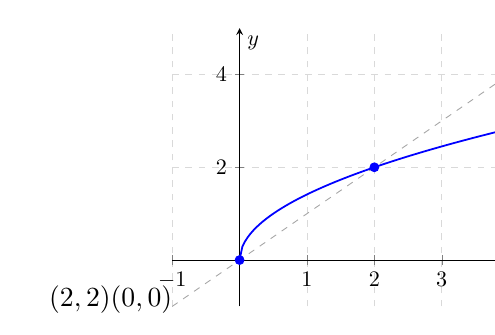
\begin{tikzpicture}[scale=0.8]
    \begin{axis}[
        axis lines = middle,
        xlabel = $x$,
        ylabel = $y$,
        xmin = -1, xmax = 5,
        ymin = -1, ymax = 5,
        grid = major,
        grid style = {dashed, gray!30},
        width = 8cm,
        height = 6cm,
    ]
    \addplot[domain=-1:5, dashed, gray!70, thin] {x};
    
    \addplot[domain=0:4, samples=100, thick, blue] {sqrt(2*x)};
    \addplot[mark=*, mark size=2pt, blue] coordinates {(0,0)};
    \addplot[mark=*, mark size=2pt, blue] coordinates {(2,2)};
    
ode[anchor=south west] at (axis cs:2,2.2) {$(2,2)$};
    
ode[anchor=north east] at (axis cs:0.2,0.2) {$(0,0)$};
    \end{axis}
\end{tikzpicture}
\end{figure}

\bigskip

\exercicio
Na figura está representado o gráfico de uma função $g$ definida em $[-1, 3]$. Represente, no referencial dado, o gráfico da função inversa $g^{-1}$.

\begin{figure}[H]
\centering
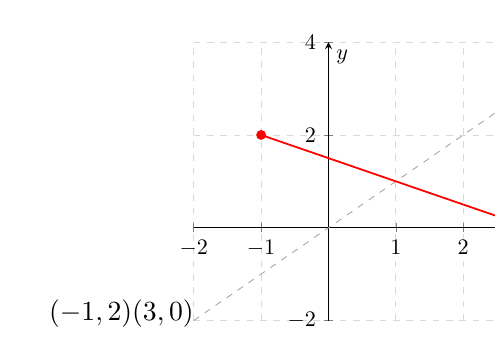
\begin{tikzpicture}[scale=0.8]
    \begin{axis}[
        axis lines = middle,
        xlabel = $x$,
        ylabel = $y$,
        xmin = -2, xmax = 4,
        ymin = -2, ymax = 4,
        grid = major,
        grid style = {dashed, gray!30},
        width = 8cm,
        height = 6cm,
    ]
    \addplot[domain=-2:4, dashed, gray!70, thin] {x};
    
    \addplot[domain=-1:3, thick, red] {-0.5*x+1.5};
    \addplot[mark=*, mark size=2pt, red] coordinates {(-1,2)};
    \addplot[mark=*, mark size=2pt, red] coordinates {(3,0)};
    
ode[anchor=south east] at (axis cs:-1,2) {$(-1,2)$};
    
ode[anchor=north west] at (axis cs:3,0) {$(3,0)$};
    \end{axis}
\end{tikzpicture}
\end{figure}
\vspace{3cm}
}
\FloatBarrier

% Exercício 53: MAT_P4FUNCOE_4FIN_GRA_003.bak_agent_20251127T121826Z.tex
% Exercise ID: MAT_P4FUNCOE_4FIN_GRA_003
% Exercise ID: MAT_P4FUNCOE_4FIN_GRA_003
% Module: MÓDULO P4 - Funções | Concept: Função Inversa | Type: Determinação Gráfica
% Difficulty: 2/5 (Fácil) | Type: desenvolvimento
% Points: 10 | Time: 10 min
% Tags: inversa, grafico, simetria, funcao_quadratica
% Author: Professor | Date: 2025-11-18
% Status: active
% Description: Dado o gráfico de ramos de funções, desenhar o gráfico da inversa

\exercicio
Na figura está representado o gráfico de uma função $f$ definida em $[0, +\infty[$. Represente, no referencial dado, o gráfico da função inversa $f^{-1}$.

\begin{figure}[ht]
\centering
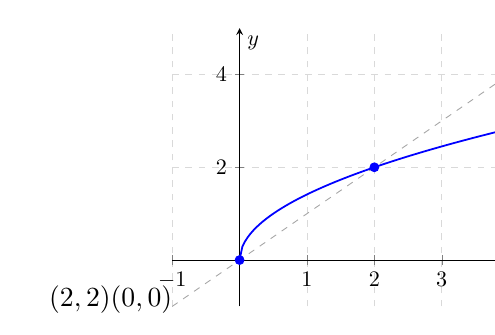
\begin{tikzpicture}[scale=0.8]
    \begin{axis}[
        axis lines = middle,
        xlabel = $x$,
        ylabel = $y$,
        xmin = -1, xmax = 5,
        ymin = -1, ymax = 5,
        grid = major,
        grid style = {dashed, gray!30},
        width = 8cm,
        height = 6cm,
    ]
    \addplot[domain=-1:5, dashed, gray!70, thin] {x};
    
    \addplot[domain=0:4, samples=100, thick, blue] {sqrt(2*x)};
    \addplot[mark=*, mark size=2pt, blue] coordinates {(0,0)};
    \addplot[mark=*, mark size=2pt, blue] coordinates {(2,2)};
    
ode[anchor=south west] at (axis cs:2,2.2) {$(2,2)$};
    
ode[anchor=north east] at (axis cs:0.2,0.2) {$(0,0)$};
    \end{axis}
\end{tikzpicture}
\end{figure}

\bigskip

\exercicio
Na figura está representado o gráfico de uma função $g$ definida em $[-1, 3]$. Represente, no referencial dado, o gráfico da função inversa $g^{-1}$.

\begin{figure}[H]
\centering
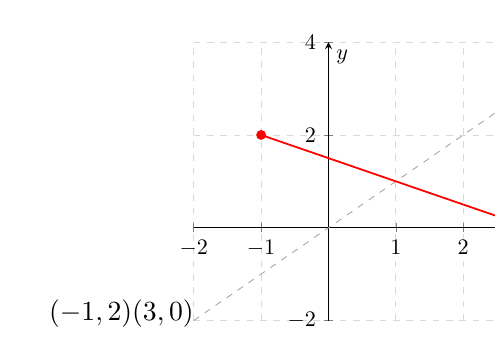
\begin{tikzpicture}[scale=0.8]
    \begin{axis}[
        axis lines = middle,
        xlabel = $x$,
        ylabel = $y$,
        xmin = -2, xmax = 4,
        ymin = -2, ymax = 4,
        grid = major,
        grid style = {dashed, gray!30},
        width = 8cm,
        height = 6cm,
    ]
    \addplot[domain=-2:4, dashed, gray!70, thin] {x};
    
    \addplot[domain=-1:3, thick, red] {-0.5*x+1.5};
    \addplot[mark=*, mark size=2pt, red] coordinates {(-1,2)};
    \addplot[mark=*, mark size=2pt, red] coordinates {(3,0)};
    
ode[anchor=south east] at (axis cs:-1,2) {$(-1,2)$};
    
ode[anchor=north west] at (axis cs:3,0) {$(3,0)$};
    \end{axis}
\end{tikzpicture}
\end{figure
\vspace{3cm}
}
\FloatBarrier

% Exercício 54: MAT_P4FUNCOE_4FIN_GRA_003.tex
% Exercise ID: MAT_P4FUNCOE_4FIN_GRA_003
% Exercise ID: MAT_P4FUNCOE_4FIN_GRA_003
% Module: MÓDULO P4 - Funções | Concept: Função Inversa | Type: Determinação Gráfica
% Difficulty: 2/5 (Fácil) | Type: desenvolvimento
% Points: 10 | Time: 10 min
% Tags: inversa, grafico, simetria, funcao_quadratica
% Author: Professor | Date: 2025-11-18
% Status: active
% Description: Dado o gráfico de ramos de funções, desenhar o gráfico da inversa

\exercicio
Na figura está representado o gráfico de uma função $f$ definida em $[0, +\infty[$. Represente, no referencial dado, o gráfico da função inversa $f^{-1}$.

\begin{figure}[ht]
\centering
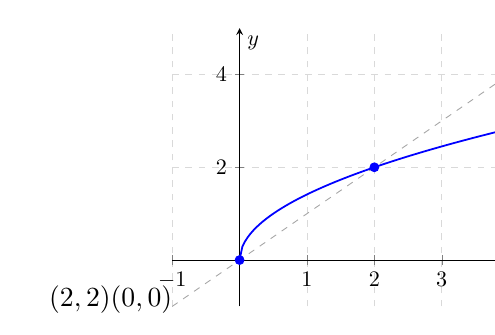
\begin{tikzpicture}[scale=0.8]
    \begin{axis}[
        axis lines = middle,
        xlabel = $x$,
        ylabel = $y$,
        xmin = -1, xmax = 5,
        ymin = -1, ymax = 5,
        grid = major,
        grid style = {dashed, gray!30},
        width = 8cm,
        height = 6cm,
    ]
    \addplot[domain=-1:5, dashed, gray!70, thin] {x};
    
    \addplot[domain=0:4, samples=100, thick, blue] {sqrt(2*x)};
    \addplot[mark=*, mark size=2pt, blue] coordinates {(0,0)};
    \addplot[mark=*, mark size=2pt, blue] coordinates {(2,2)};
    
ode[anchor=south west] at (axis cs:2,2.2) {$(2,2)$};
    
ode[anchor=north east] at (axis cs:0.2,0.2) {$(0,0)$};
    \end{axis}
\end{tikzpicture}
\end{figure}

\bigskip

\exercicio
Na figura está representado o gráfico de uma função $g$ definida em $[-1, 3]$. Represente, no referencial dado, o gráfico da função inversa $g^{-1}$.

\begin{figure}[H]
\centering
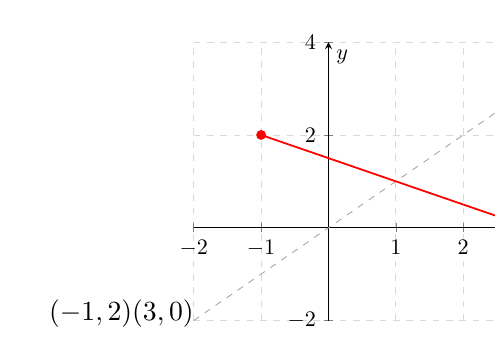
\begin{tikzpicture}[scale=0.8]
    \begin{axis}[
        axis lines = middle,
        xlabel = $x$,
        ylabel = $y$,
        xmin = -2, xmax = 4,
        ymin = -2, ymax = 4,
        grid = major,
        grid style = {dashed, gray!30},
        width = 8cm,
        height = 6cm,
    ]
    \addplot[domain=-2:4, dashed, gray!70, thin] {x};
    
    \addplot[domain=-1:3, thick, red] {-0.5*x+1.5};
    \addplot[mark=*, mark size=2pt, red] coordinates {(-1,2)};
    \addplot[mark=*, mark size=2pt, red] coordinates {(3,0)};
    
ode[anchor=south east] at (axis cs:-1,2) {$(-1,2)$};
    
ode[anchor=north west] at (axis cs:3,0) {$(3,0)$};
    \end{axis}
\end{tikzpicture}
\end{figure
\vspace{3cm}
}
\FloatBarrier

% Exercício 55: MAT_P4FUNCOE_4FIN_GRA_004.agentfix.tex
% Exercise ID: MAT_P4FUNCOE_4FIN_GRA_004
% Exercise ID: MAT_P4FUNCOE_4FIN_GRA_004
% Module: MÓDULO P4 - Funções | Concept: Função Inversa | Type: Determinação Gráfica
% Difficulty: 2/5 (Fácil) | Type: desenvolvimento
% Points: 10 | Time: 10 min
% Tags: inversa, grafico, simetria, funcao_quadratica
% Author: Professor | Date: 2025-11-18
% Status: active
% Description: Dado o gráfico de ramos de funções, desenhar o gráfico da inversa

\exercicio
Na figura está representado o gráfico de uma função $f$ definida em $[1, 4]$. Represente, no referencial dado, o gráfico da função inversa $f^{-1}$.

\begin{figure}[ht]
\centering
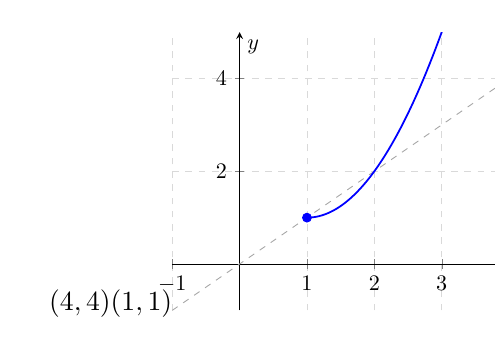
\begin{tikzpicture}[scale=0.8]
    \begin{axis}[
        axis lines = middle,
        xlabel = $x$,
        ylabel = $y$,
        xmin = -1, xmax = 5,
        ymin = -1, ymax = 5,
        grid = major,
        grid style = {dashed, gray!30},
        width = 8cm,
        height = 6cm,
    ]
    \addplot[domain=-1:5, dashed, gray!70, thin] {x};
    
    \addplot[domain=1:4, samples=100, thick, blue] {(x-1)^2 + 1};
    \addplot[mark=*, mark size=2pt, blue] coordinates {(1,1)};
    \addplot[mark=*, mark size=2pt, blue] coordinates {(4,10/2)};
    
ode[anchor=west] at (axis cs:4,4.2) {$(4,4)$};
    
ode[anchor=north east] at (axis cs:1,0.8) {$(1,1)$};
    \end{axis}
\end{tikzpicture}
\end{figure}

\bigskip

\exercicio
Na figura está representado o gráfico de uma função $g$ definida em $]0, 4]$. Represente, no referencial dado, o gráfico da função inversa $g^{-1}$.

\begin{figure}[H]
\centering
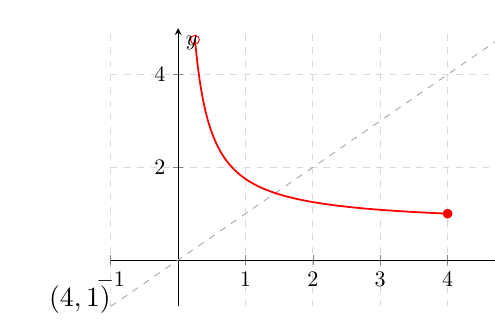
\begin{tikzpicture}[scale=0.8]
    \begin{axis}[
        axis lines = middle,
        xlabel = $x$,
        ylabel = $y$,
        xmin = -1, xmax = 5,
        ymin = -1, ymax = 5,
        grid = major,
        grid style = {dashed, gray!30},
        width = 8cm,
        height = 6cm,
    ]
    \addplot[domain=-1:5, dashed, gray!70, thin] {x};
    
    \addplot[domain=0.25:4, samples=100, thick, red] {1/x + 0.75};
    \addplot[mark=o, mark size=2pt, red] coordinates {(0.25,4.75)};
    \addplot[mark=*, mark size=2pt, red] coordinates {(4,1)};
    
ode[anchor=south] at (axis cs:4,1.2) {$(4,1)$};
    \end{axis}
\end{tikzpicture}
\end{figure}
\vspace{3cm}
}
\FloatBarrier

% Exercício 56: MAT_P4FUNCOE_4FIN_GRA_004.bak_agent_20251127T121826Z.tex
% Exercise ID: MAT_P4FUNCOE_4FIN_GRA_004
% Exercise ID: MAT_P4FUNCOE_4FIN_GRA_004
% Module: MÓDULO P4 - Funções | Concept: Função Inversa | Type: Determinação Gráfica
% Difficulty: 2/5 (Fácil) | Type: desenvolvimento
% Points: 10 | Time: 10 min
% Tags: inversa, grafico, simetria, funcao_quadratica
% Author: Professor | Date: 2025-11-18
% Status: active
% Description: Dado o gráfico de ramos de funções, desenhar o gráfico da inversa

\exercicio
Na figura está representado o gráfico de uma função $f$ definida em $[1, 4]$. Represente, no referencial dado, o gráfico da função inversa $f^{-1}$.

\begin{figure}[ht]
\centering
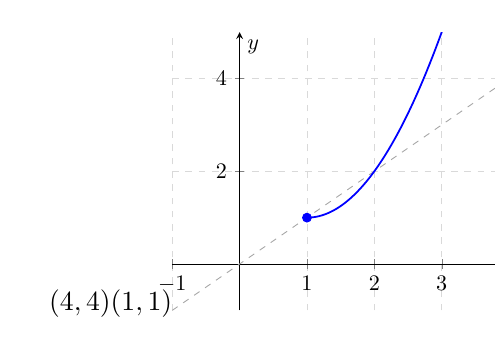
\begin{tikzpicture}[scale=0.8]
    \begin{axis}[
        axis lines = middle,
        xlabel = $x$,
        ylabel = $y$,
        xmin = -1, xmax = 5,
        ymin = -1, ymax = 5,
        grid = major,
        grid style = {dashed, gray!30},
        width = 8cm,
        height = 6cm,
    ]
    \addplot[domain=-1:5, dashed, gray!70, thin] {x};
    
    \addplot[domain=1:4, samples=100, thick, blue] {(x-1)^2 + 1};
    \addplot[mark=*, mark size=2pt, blue] coordinates {(1,1)};
    \addplot[mark=*, mark size=2pt, blue] coordinates {(4,10/2)};
    
ode[anchor=west] at (axis cs:4,4.2) {$(4,4)$};
    
ode[anchor=north east] at (axis cs:1,0.8) {$(1,1)$};
    \end{axis}
\end{tikzpicture}
\end{figure}

\bigskip

\exercicio
Na figura está representado o gráfico de uma função $g$ definida em $]0, 4]$. Represente, no referencial dado, o gráfico da função inversa $g^{-1}$.

\begin{figure}[H]
\centering
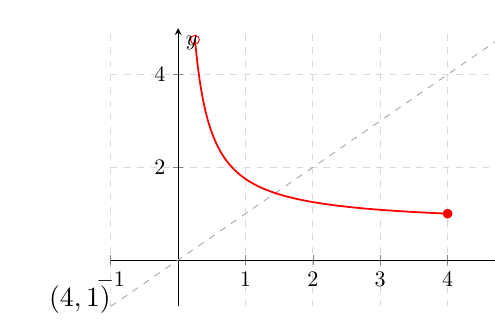
\begin{tikzpicture}[scale=0.8]
    \begin{axis}[
        axis lines = middle,
        xlabel = $x$,
        ylabel = $y$,
        xmin = -1, xmax = 5,
        ymin = -1, ymax = 5,
        grid = major,
        grid style = {dashed, gray!30},
        width = 8cm,
        height = 6cm,
    ]
    \addplot[domain=-1:5, dashed, gray!70, thin] {x};
    
    \addplot[domain=0.25:4, samples=100, thick, red] {1/x + 0.75};
    \addplot[mark=o, mark size=2pt, red] coordinates {(0.25,4.75)};
    \addplot[mark=*, mark size=2pt, red] coordinates {(4,1)};
    
ode[anchor=south] at (axis cs:4,1.2) {$(4,1)$};
    \end{axis}
\end{tikzpicture}
\end{figure
\vspace{3cm}
}
\FloatBarrier

% Exercício 57: MAT_P4FUNCOE_4FIN_GRA_004.tex
% Exercise ID: MAT_P4FUNCOE_4FIN_GRA_004
% Exercise ID: MAT_P4FUNCOE_4FIN_GRA_004
% Module: MÓDULO P4 - Funções | Concept: Função Inversa | Type: Determinação Gráfica
% Difficulty: 2/5 (Fácil) | Type: desenvolvimento
% Points: 10 | Time: 10 min
% Tags: inversa, grafico, simetria, funcao_quadratica
% Author: Professor | Date: 2025-11-18
% Status: active
% Description: Dado o gráfico de ramos de funções, desenhar o gráfico da inversa

\exercicio
Na figura está representado o gráfico de uma função $f$ definida em $[1, 4]$. Represente, no referencial dado, o gráfico da função inversa $f^{-1}$.

\begin{figure}[ht]
\centering
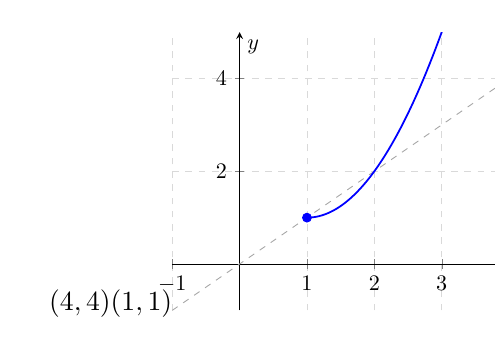
\begin{tikzpicture}[scale=0.8]
    \begin{axis}[
        axis lines = middle,
        xlabel = $x$,
        ylabel = $y$,
        xmin = -1, xmax = 5,
        ymin = -1, ymax = 5,
        grid = major,
        grid style = {dashed, gray!30},
        width = 8cm,
        height = 6cm,
    ]
    \addplot[domain=-1:5, dashed, gray!70, thin] {x};
    
    \addplot[domain=1:4, samples=100, thick, blue] {(x-1)^2 + 1};
    \addplot[mark=*, mark size=2pt, blue] coordinates {(1,1)};
    \addplot[mark=*, mark size=2pt, blue] coordinates {(4,10/2)};
    
ode[anchor=west] at (axis cs:4,4.2) {$(4,4)$};
    
ode[anchor=north east] at (axis cs:1,0.8) {$(1,1)$};
    \end{axis}
\end{tikzpicture}
\end{figure}

\bigskip

\exercicio
Na figura está representado o gráfico de uma função $g$ definida em $]0, 4]$. Represente, no referencial dado, o gráfico da função inversa $g^{-1}$.

\begin{figure}[H]
\centering
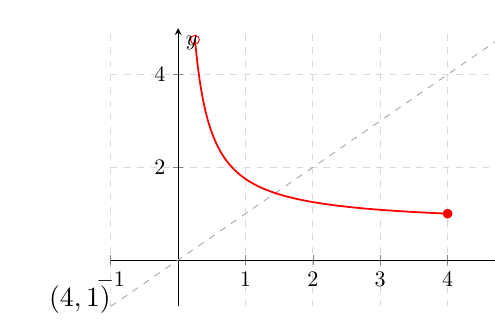
\begin{tikzpicture}[scale=0.8]
    \begin{axis}[
        axis lines = middle,
        xlabel = $x$,
        ylabel = $y$,
        xmin = -1, xmax = 5,
        ymin = -1, ymax = 5,
        grid = major,
        grid style = {dashed, gray!30},
        width = 8cm,
        height = 6cm,
    ]
    \addplot[domain=-1:5, dashed, gray!70, thin] {x};
    
    \addplot[domain=0.25:4, samples=100, thick, red] {1/x + 0.75};
    \addplot[mark=o, mark size=2pt, red] coordinates {(0.25,4.75)};
    \addplot[mark=*, mark size=2pt, red] coordinates {(4,1)};
    
ode[anchor=south] at (axis cs:4,1.2) {$(4,1)$};
    \end{axis}
\end{tikzpicture}
\end{figure
\vspace{3cm}
}
\FloatBarrier

% Exercício 58: MAT_P4FUNCOE_4FIN_GRA_005.agentfix.tex
% Exercise ID: MAT_P4FUNCOE_4FIN_GRA_005
% Exercise ID: MAT_P4FUNCOE_4FIN_GRA_005
% Module: MÓDULO P4 - Funções | Concept: Função Inversa | Type: Determinação Gráfica
% Difficulty: 2/5 (Fácil) | Type: desenvolvimento
% Points: 10 | Time: 10 min
% Tags: inversa, grafico, simetria, funcao_quadratica
% Author: Professor | Date: 2025-11-18
% Status: active
% Description: Dado o gráfico de ramos de funções, desenhar o gráfico da inversa

\exercicio
Na figura está representado o gráfico de uma função $f$ definida em $[-2, 2]$. Represente, no referencial dado, o gráfico da função inversa $f^{-1}$.

\begin{figure}[ht]
\centering
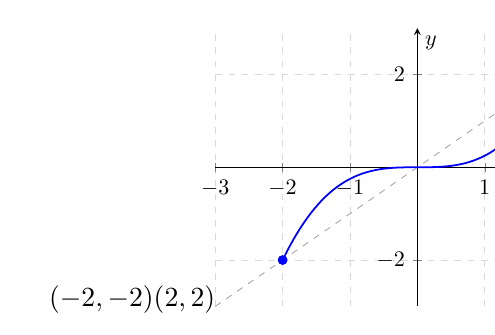
\begin{tikzpicture}[scale=0.8]
    \begin{axis}[
        axis lines = middle,
        xlabel = $x$,
        ylabel = $y$,
        xmin = -3, xmax = 3,
        ymin = -3, ymax = 3,
        grid = major,
        grid style = {dashed, gray!30},
        width = 8cm,
        height = 6cm,
    ]
    \addplot[domain=-3:3, dashed, gray!70, thin] {x};
    
    \addplot[domain=-2:2, samples=100, thick, blue] {x^3/4};
    \addplot[mark=*, mark size=2pt, blue] coordinates {(-2,-2)};
    \addplot[mark=*, mark size=2pt, blue] coordinates {(2,2)};
    
ode[anchor=north east] at (axis cs:-2,-2) {$(-2,-2)$};
    
ode[anchor=south west] at (axis cs:2,2) {$(2,2)$};
    \end{axis}
\end{tikzpicture}
\end{figure}

\bigskip

\exercicio
Na figura está representado o gráfico de uma função $g$ definida em $[0, 3]$. Represente, no referencial dado, o gráfico da função inversa $g^{-1}$.

\begin{figure}[H]
\centering
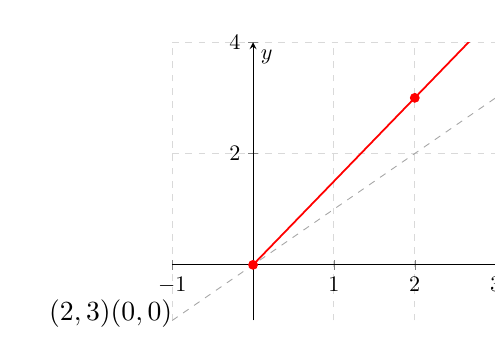
\begin{tikzpicture}[scale=0.8]
    \begin{axis}[
        axis lines = middle,
        xlabel = $x$,
        ylabel = $y$,
        xmin = -1, xmax = 4,
        ymin = -1, ymax = 4,
        grid = major,
        grid style = {dashed, gray!30},
        width = 8cm,
        height = 6cm,
    ]
    \addplot[domain=-1:4, dashed, gray!70, thin] {x};
    
    \addplot[domain=0:3, thick, red] {3*x/2};
    \addplot[mark=*, mark size=2pt, red] coordinates {(0,0)};
    \addplot[mark=*, mark size=2pt, red] coordinates {(2,3)};
    
ode[anchor=south west] at (axis cs:2,3.1) {$(2,3)$};
    
ode[anchor=north east] at (axis cs:0.2,0.2) {$(0,0)$};
    \end{axis}
\end{tikzpicture}
\end{figure}
\vspace{3cm}
}
\FloatBarrier

% Exercício 59: MAT_P4FUNCOE_4FIN_GRA_005.bak_agent_20251127T121826Z.tex
% Exercise ID: MAT_P4FUNCOE_4FIN_GRA_005
% Exercise ID: MAT_P4FUNCOE_4FIN_GRA_005
% Module: MÓDULO P4 - Funções | Concept: Função Inversa | Type: Determinação Gráfica
% Difficulty: 2/5 (Fácil) | Type: desenvolvimento
% Points: 10 | Time: 10 min
% Tags: inversa, grafico, simetria, funcao_quadratica
% Author: Professor | Date: 2025-11-18
% Status: active
% Description: Dado o gráfico de ramos de funções, desenhar o gráfico da inversa

\exercicio
Na figura está representado o gráfico de uma função $f$ definida em $[-2, 2]$. Represente, no referencial dado, o gráfico da função inversa $f^{-1}$.

\begin{figure}[ht]
\centering
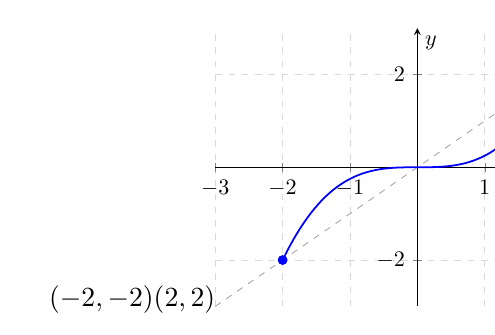
\begin{tikzpicture}[scale=0.8]
    \begin{axis}[
        axis lines = middle,
        xlabel = $x$,
        ylabel = $y$,
        xmin = -3, xmax = 3,
        ymin = -3, ymax = 3,
        grid = major,
        grid style = {dashed, gray!30},
        width = 8cm,
        height = 6cm,
    ]
    \addplot[domain=-3:3, dashed, gray!70, thin] {x};
    
    \addplot[domain=-2:2, samples=100, thick, blue] {x^3/4};
    \addplot[mark=*, mark size=2pt, blue] coordinates {(-2,-2)};
    \addplot[mark=*, mark size=2pt, blue] coordinates {(2,2)};
    
ode[anchor=north east] at (axis cs:-2,-2) {$(-2,-2)$};
    
ode[anchor=south west] at (axis cs:2,2) {$(2,2)$};
    \end{axis}
\end{tikzpicture}
\end{figure}

\bigskip

\exercicio
Na figura está representado o gráfico de uma função $g$ definida em $[0, 3]$. Represente, no referencial dado, o gráfico da função inversa $g^{-1}$.

\begin{figure}[H]
\centering
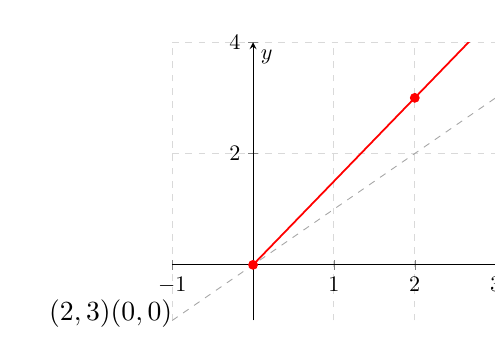
\begin{tikzpicture}[scale=0.8]
    \begin{axis}[
        axis lines = middle,
        xlabel = $x$,
        ylabel = $y$,
        xmin = -1, xmax = 4,
        ymin = -1, ymax = 4,
        grid = major,
        grid style = {dashed, gray!30},
        width = 8cm,
        height = 6cm,
    ]
    \addplot[domain=-1:4, dashed, gray!70, thin] {x};
    
    \addplot[domain=0:3, thick, red] {3*x/2};
    \addplot[mark=*, mark size=2pt, red] coordinates {(0,0)};
    \addplot[mark=*, mark size=2pt, red] coordinates {(2,3)};
    
ode[anchor=south west] at (axis cs:2,3.1) {$(2,3)$};
    
ode[anchor=north east] at (axis cs:0.2,0.2) {$(0,0)$};
    \end{axis}
\end{tikzpicture}
\end{figure
\vspace{3cm}
}
\FloatBarrier

% Exercício 60: MAT_P4FUNCOE_4FIN_GRA_005.tex
% Exercise ID: MAT_P4FUNCOE_4FIN_GRA_005
% Exercise ID: MAT_P4FUNCOE_4FIN_GRA_005
% Module: MÓDULO P4 - Funções | Concept: Função Inversa | Type: Determinação Gráfica
% Difficulty: 2/5 (Fácil) | Type: desenvolvimento
% Points: 10 | Time: 10 min
% Tags: inversa, grafico, simetria, funcao_quadratica
% Author: Professor | Date: 2025-11-18
% Status: active
% Description: Dado o gráfico de ramos de funções, desenhar o gráfico da inversa

\exercicio
Na figura está representado o gráfico de uma função $f$ definida em $[-2, 2]$. Represente, no referencial dado, o gráfico da função inversa $f^{-1}$.

\begin{figure}[ht]
\centering
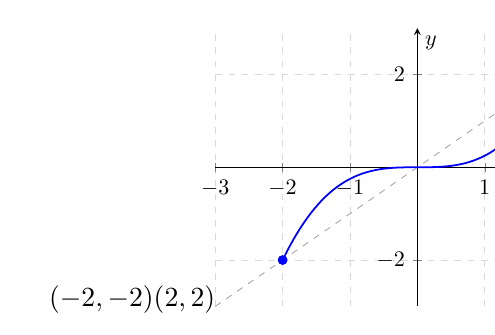
\begin{tikzpicture}[scale=0.8]
    \begin{axis}[
        axis lines = middle,
        xlabel = $x$,
        ylabel = $y$,
        xmin = -3, xmax = 3,
        ymin = -3, ymax = 3,
        grid = major,
        grid style = {dashed, gray!30},
        width = 8cm,
        height = 6cm,
    ]
    \addplot[domain=-3:3, dashed, gray!70, thin] {x};
    
    \addplot[domain=-2:2, samples=100, thick, blue] {x^3/4};
    \addplot[mark=*, mark size=2pt, blue] coordinates {(-2,-2)};
    \addplot[mark=*, mark size=2pt, blue] coordinates {(2,2)};
    
ode[anchor=north east] at (axis cs:-2,-2) {$(-2,-2)$};
    
ode[anchor=south west] at (axis cs:2,2) {$(2,2)$};
    \end{axis}
\end{tikzpicture}
\end{figure}

\bigskip

\exercicio
Na figura está representado o gráfico de uma função $g$ definida em $[0, 3]$. Represente, no referencial dado, o gráfico da função inversa $g^{-1}$.

\begin{figure}[H]
\centering
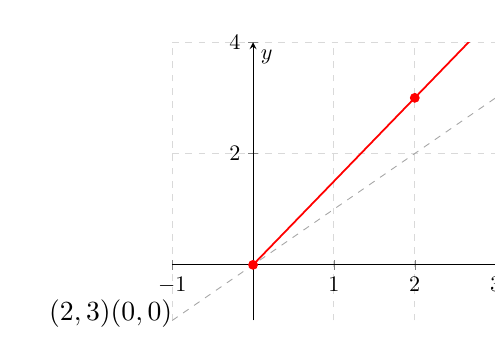
\begin{tikzpicture}[scale=0.8]
    \begin{axis}[
        axis lines = middle,
        xlabel = $x$,
        ylabel = $y$,
        xmin = -1, xmax = 4,
        ymin = -1, ymax = 4,
        grid = major,
        grid style = {dashed, gray!30},
        width = 8cm,
        height = 6cm,
    ]
    \addplot[domain=-1:4, dashed, gray!70, thin] {x};
    
    \addplot[domain=0:3, thick, red] {3*x/2};
    \addplot[mark=*, mark size=2pt, red] coordinates {(0,0)};
    \addplot[mark=*, mark size=2pt, red] coordinates {(2,3)};
    
ode[anchor=south west] at (axis cs:2,3.1) {$(2,3)$};
    
ode[anchor=north east] at (axis cs:0.2,0.2) {$(0,0)$};
    \end{axis}
\end{tikzpicture}
\end{figure
\vspace{3cm}
}
\FloatBarrier

% Exercício 61: MAT_P4FUNCOE_4FX_DGX_001.tex
% Exercise ID: MAT_P4FUNCOE_4FX_DGX_001
% Module: MÓDULO P4 - Funções | Concept: Função Inversa | Type: Determinação Gráfica da Função Inversa
% Difficulty: 4/5 (Difícil) | Format: standard
% Tags: sobrejetividade, inversa, grafico, representacao_grafica, bissectriz, injetividade, simetria, grafico, simetria
% Author: Test Agent | Date: 2025-11-26
% Status: active

\exercicio{Determine graficamente a função inversa de f(x) = x^2 + 2, para x  0.}
\FloatBarrier

% Exercício 62: MAT_P4FUNCOE_4FIN_TRH_001.agentfix.tex
% Exercise ID: MAT_P4FUNCOE_4FIN_TRH_001
% Module: MÓDULO P4 - Funções | Concept: Função Inversa | Type: Teste da Reta Horizontal
% Difficulty: 2/5 (Fácil) | Type: desenvolvimento
% Points: 10 | Time: 10 min
% Tags: inversa, injetividade, teste_reta_horizontal, grafico
% Author: Professor | Date: 2025-11-18
% Status: active
% Description: Determinar quais funções são invertíveis usando teste da reta horizontal

\exercicio
Considere as funções representadas nas figuras seguintes:

\begin{figure}[H]
\centering
\begin{minipage}{0.45\textwidth}
\centering
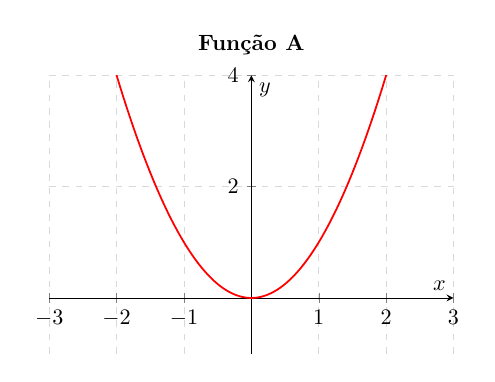
\begin{tikzpicture}[scale=0.8]
    \begin{axis}[
        axis lines = middle,
        xlabel = $x$,
        ylabel = $y$,
        xmin = -3, xmax = 3,
        ymin = -1, ymax = 4,
        grid = major,
        grid style = {dashed, gray!30},
        width = 8cm,
        height = 6cm,
        title = {Função A},
        title style = {font=\bfseries},
    ]
    \addplot[domain=-2.5:2.5, samples=100, thick, red] {x^2};
    \end{axis}
\end{tikzpicture}
\end{minipage}
\hfill
\begin{minipage}{0.45\textwidth}
\centering
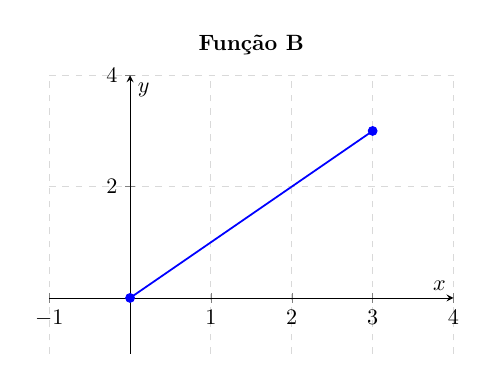
\begin{tikzpicture}[scale=0.8]
    \begin{axis}[
        axis lines = middle,
        xlabel = $x$,
        ylabel = $y$,
        xmin = -1, xmax = 4,
        ymin = -1, ymax = 4,
        grid = major,
        grid style = {dashed, gray!30},
        width = 8cm,
        height = 6cm,
        title = {Função B},
        title style = {font=\bfseries},
    ]
    \addplot[domain=0:3, samples=100, thick, blue] {x};
    \addplot[mark=*, mark size=2pt, blue] coordinates {(0,0)};
    \addplot[mark=*, mark size=2pt, blue] coordinates {(3,3)};
    \end{axis}
\end{tikzpicture}
\end{minipage}
\end{figure}

Quais das duas funções são invertíveis (isto é, cuja inversa também é uma função)? Justifique usando o teste da reta horizontal.

\vspace{3cm}
\FloatBarrier

% Exercício 63: MAT_P4FUNCOE_4FIN_TRH_001.bak_agent_20251127T121826Z.tex
% Exercise ID: MAT_P4FUNCOE_4FIN_TRH_001
% Module: MÓDULO P4 - Funções | Concept: Função Inversa | Type: Teste da Reta Horizontal
% Difficulty: 2/5 (Fácil) | Type: desenvolvimento
% Points: 10 | Time: 10 min
% Tags: inversa, injetividade, teste_reta_horizontal, grafico
% Author: Professor | Date: 2025-11-18
% Status: active
% Description: Determinar quais funções são invertíveis usando teste da reta horizontal

\exercicio
Considere as funções representadas nas figuras seguintes:

\begin{figure}[H]
\centering
\begin{minipage}{0.45\textwidth}
\centering
\begin{tikzpicture}[scale=0.8]
    \begin{axis}[
        axis lines = middle,
        xlabel = $x$,
        ylabel = $y$,
        xmin = -3, xmax = 3,
        ymin = -1, ymax = 4,
        grid = major,
        grid style = {dashed, gray!30},
        width = 8cm,
        height = 6cm,
        title = {Função A},
        title style = {font=\bfseries},
    ]
    \addplot[domain=-2.5:2.5, samples=100, thick, red] {x^2};
    \end{axis}
\end{tikzpicture}
\end{minipage}
\hfill
\begin{minipage}{0.45\textwidth}
\centering
\begin{tikzpicture}[scale=0.8]
    \begin{axis}[
        axis lines = middle,
        xlabel = $x$,
        ylabel = $y$,
        xmin = -1, xmax = 4,
        ymin = -1, ymax = 4,
        grid = major,
        grid style = {dashed, gray!30},
        width = 8cm,
        height = 6cm,
        title = {Função B},
        title style = {font=\bfseries},
    ]
    \addplot[domain=0:3, samples=100, thick, blue] {x};
    \addplot[mark=*, mark size=2pt, blue] coordinates {(0,0)};
    \addplot[mark=*, mark size=2pt, blue] coordinates {(3,3)};
    \end{axis}
\end{tikzpicture}
\end{minipage}
\end{figure}

Quais das duas funções são invertíveis (isto é, cuja inversa também é uma função)? Justifique usando o teste da reta horizontal.

\vspace{3cm}
\FloatBarrier

% Exercício 64: MAT_P4FUNCOE_4FIN_TRH_001.tex
% Exercise ID: MAT_P4FUNCOE_4FIN_TRH_001
% Module: MÓDULO P4 - Funções | Concept: Função Inversa | Type: Teste da Reta Horizontal
% Difficulty: 2/5 (Fácil) | Type: desenvolvimento
% Points: 10 | Time: 10 min
% Tags: inversa, injetividade, teste_reta_horizontal, grafico
% Author: Professor | Date: 2025-11-18
% Status: active
% Description: Determinar quais funções são invertíveis usando teste da reta horizontal

\exercicio
Considere as funções representadas nas figuras seguintes:

\begin{figure}[H]
\centering
\begin{minipage}{0.45\textwidth}
\centering
\begin{tikzpicture}[scale=0.8]
    \begin{axis}[
        axis lines = middle,
        xlabel = $x$,
        ylabel = $y$,
        xmin = -3, xmax = 3,
        ymin = -1, ymax = 4,
        grid = major,
        grid style = {dashed, gray!30},
        width = 8cm,
        height = 6cm,
        title = {Função A},
        title style = {font=\bfseries},
    ]
    \addplot[domain=-2.5:2.5, samples=100, thick, red] {x^2};
    \end{axis}
\end{tikzpicture}
\end{minipage}
\hfill
\begin{minipage}{0.45\textwidth}
\centering
\begin{tikzpicture}[scale=0.8]
    \begin{axis}[
        axis lines = middle,
        xlabel = $x$,
        ylabel = $y$,
        xmin = -1, xmax = 4,
        ymin = -1, ymax = 4,
        grid = major,
        grid style = {dashed, gray!30},
        width = 8cm,
        height = 6cm,
        title = {Função B},
        title style = {font=\bfseries},
    ]
    \addplot[domain=0:3, samples=100, thick, blue] {x};
    \addplot[mark=*, mark size=2pt, blue] coordinates {(0,0)};
    \addplot[mark=*, mark size=2pt, blue] coordinates {(3,3)};
    \end{axis}
\end{tikzpicture}
\end{minipage}
\end{figure}

Quais das duas funções são invertíveis (isto é, cuja inversa também é uma função)? Justifique usando o teste da reta horizontal.

\vspace{3cm}
\FloatBarrier

% Exercício 65: MAT_P4FUNCOE_4FIN_TRH_002.agentfix.tex
% Exercise ID: MAT_P4FUNCOE_4FIN_TRH_002
% Exercise ID: MAT_P4FUNCOE_4FIN_TRH_002
% Module: MÓDULO P4 - Funções | Concept: Função Inversa | Type: Teste da Reta Horizontal
% Difficulty: 2/5 (Fácil) | Type: desenvolvimento
% Points: 10 | Time: 10 min
% Tags: inversa, injetividade, teste_reta_horizontal, grafico
% Author: Professor | Date: 2025-11-18
% Status: active
% Description: Determinar quais funções são invertíveis usando teste da reta horizontal

\exercicio
Considere as funções representadas nas figuras seguintes:

\begin{figure}[H]
\centering
\begin{minipage}{0.45\textwidth}
\centering
\begin{tikzpicture}[scale=0.8]
    \begin{axis}[
        axis lines = middle,
        xlabel = $x$,
        ylabel = $y$,
        xmin = -3, xmax = 3,
        ymin = -2, ymax = 4,
        grid = major,
        grid style = {dashed, gray!30},
        width = 8cm,
        height = 6cm,
        title = {Função C},
        title style = {font=\bfseries},
    ]
    \addplot[domain=-2:2, samples=100, thick, red] {x^2-4};
    \end{axis}
\end{tikzpicture}
\end{minipage}
\hfill
\begin{minipage}{0.45\textwidth}
\centering
\begin{tikzpicture}[scale=0.8]
    \begin{axis}[
        axis lines = middle,
        xlabel = $x$,
        ylabel = $y$,
        xmin = -1, xmax = 4,
        ymin = -1, ymax = 5,
        grid = major,
        grid style = {dashed, gray!30},
        width = 8cm,
        height = 6cm,
        title = {Função D},
        title style = {font=\bfseries},
    ]
    \addplot[domain=0:3.5, samples=100, thick, blue] {sqrt(x)};
    \addplot[mark=*, mark size=2pt, blue] coordinates {(0,0)};
    \end{axis}
\end{tikzpicture}
\end{minipage}
\end{figure}



Quais das duas funções são invertíveis (isto é, cuja inversa também é uma função)? Justifique usando o teste da reta horizontal.

\vspace{3cm}
\FloatBarrier

% Exercício 66: MAT_P4FUNCOE_4FIN_TRH_002.bak_agent_20251127T121826Z.tex
% Exercise ID: MAT_P4FUNCOE_4FIN_TRH_002
% Exercise ID: MAT_P4FUNCOE_4FIN_TRH_002
% Module: MÓDULO P4 - Funções | Concept: Função Inversa | Type: Teste da Reta Horizontal
% Difficulty: 2/5 (Fácil) | Type: desenvolvimento
% Points: 10 | Time: 10 min
% Tags: inversa, injetividade, teste_reta_horizontal, grafico
% Author: Professor | Date: 2025-11-18
% Status: active
% Description: Determinar quais funções são invertíveis usando teste da reta horizontal

\exercicio
Considere as funções representadas nas figuras seguintes:

\begin{figure}[H]
\centering
\begin{minipage}{0.45\textwidth}
\centering
\begin{tikzpicture}[scale=0.8]
    \begin{axis}[
        axis lines = middle,
        xlabel = $x$,
        ylabel = $y$,
        xmin = -3, xmax = 3,
        ymin = -2, ymax = 4,
        grid = major,
        grid style = {dashed, gray!30},
        width = 8cm,
        height = 6cm,
        title = {Função C},
        title style = {font=\bfseries},
    ]
    \addplot[domain=-2:2, samples=100, thick, red] {x^2-4};
    \end{axis}
\end{tikzpicture}
\end{minipage}
\hfill
\begin{minipage}{0.45\textwidth}
\centering
\begin{tikzpicture}[scale=0.8]
    \begin{axis}[
        axis lines = middle,
        xlabel = $x$,
        ylabel = $y$,
        xmin = -1, xmax = 4,
        ymin = -1, ymax = 5,
        grid = major,
        grid style = {dashed, gray!30},
        width = 8cm,
        height = 6cm,
        title = {Função D},
        title style = {font=\bfseries},
    ]
    \addplot[domain=0:3.5, samples=100, thick, blue] {sqrt(x)};
    \addplot[mark=*, mark size=2pt, blue] coordinates {(0,0)};
    \end{axis}
\end{tikzpicture}
\end{minipage}
\end{figure}



Quais das duas funções são invertíveis (isto é, cuja inversa também é uma função)? Justifique usando o teste da reta horizontal.

\vspace{3cm}
\FloatBarrier

% Exercício 67: MAT_P4FUNCOE_4FIN_TRH_002.tex
% Exercise ID: MAT_P4FUNCOE_4FIN_TRH_002
% Exercise ID: MAT_P4FUNCOE_4FIN_TRH_002
% Module: MÓDULO P4 - Funções | Concept: Função Inversa | Type: Teste da Reta Horizontal
% Difficulty: 2/5 (Fácil) | Type: desenvolvimento
% Points: 10 | Time: 10 min
% Tags: inversa, injetividade, teste_reta_horizontal, grafico
% Author: Professor | Date: 2025-11-18
% Status: active
% Description: Determinar quais funções são invertíveis usando teste da reta horizontal

\exercicio
Considere as funções representadas nas figuras seguintes:

\begin{figure}[H]
\centering
\begin{minipage}{0.45\textwidth}
\centering
\begin{tikzpicture}[scale=0.8]
    \begin{axis}[
        axis lines = middle,
        xlabel = $x$,
        ylabel = $y$,
        xmin = -3, xmax = 3,
        ymin = -2, ymax = 4,
        grid = major,
        grid style = {dashed, gray!30},
        width = 8cm,
        height = 6cm,
        title = {Função C},
        title style = {font=\bfseries},
    ]
    \addplot[domain=-2:2, samples=100, thick, red] {x^2-4};
    \end{axis}
\end{tikzpicture}
\end{minipage}
\hfill
\begin{minipage}{0.45\textwidth}
\centering
\begin{tikzpicture}[scale=0.8]
    \begin{axis}[
        axis lines = middle,
        xlabel = $x$,
        ylabel = $y$,
        xmin = -1, xmax = 4,
        ymin = -1, ymax = 5,
        grid = major,
        grid style = {dashed, gray!30},
        width = 8cm,
        height = 6cm,
        title = {Função D},
        title style = {font=\bfseries},
    ]
    \addplot[domain=0:3.5, samples=100, thick, blue] {sqrt(x)};
    \addplot[mark=*, mark size=2pt, blue] coordinates {(0,0)};
    \end{axis}
\end{tikzpicture}
\end{minipage}
\end{figure}



Quais das duas funções são invertíveis (isto é, cuja inversa também é uma função)? Justifique usando o teste da reta horizontal.

\vspace{3cm}
\FloatBarrier

% Exercício 68: MAT_P4FUNCOE_4FIN_TRH_003.agentfix.tex
% Exercise ID: MAT_P4FUNCOE_4FIN_TRH_003
% Exercise ID: MAT_P4FUNCOE_4FIN_TRH_003
% Module: MÓDULO P4 - Funções | Concept: Função Inversa | Type: Teste da Reta Horizontal
% Difficulty: 2/5 (Fácil) | Type: desenvolvimento
% Points: 10 | Time: 10 min
% Tags: inversa, injetividade, teste_reta_horizontal, grafico
% Author: Professor | Date: 2025-11-18
% Status: active
% Description: Determinar quais funções são invertíveis usando teste da reta horizontal

\exercicio
Considere as funções representadas nas figuras seguintes:

\begin{figure}[H]
\centering
\begin{minipage}{0.45\textwidth}
\centering
\begin{tikzpicture}[scale=0.8]
    \begin{axis}[
        axis lines = middle,
        xlabel = $x$,
        ylabel = $y$,
        xmin = -4, xmax = 4,
        ymin = -2, ymax = 2,
        grid = major,
        grid style = {dashed, gray!30},
        width = 8cm,
        height = 6cm,
        title = {Função E},
        title style = {font=\bfseries},
    ]
    \addplot[domain=-3.14:3.14, samples=200, thick, red] {sin(deg(x))};
    \end{axis}
\end{tikzpicture}
\end{minipage}
\hfill
\begin{minipage}{0.45\textwidth}
\centering
\begin{tikzpicture}[scale=0.8]
    \begin{axis}[
        axis lines = middle,
        xlabel = $x$,
        ylabel = $y$,
        xmin = -1, xmax = 4,
        ymin = -1, ymax = 4,
        grid = major,
        grid style = {dashed, gray!30},
        width = 8cm,
        height = 6cm,
        title = {Função F},
        title style = {font=\bfseries},
    ]
    \addplot[domain=0:3, thick, blue] {2*x};
    \addplot[mark=*, mark size=2pt, blue] coordinates {(0,0)};
    \addplot[mark=*, mark size=2pt, blue] coordinates {(3,6)};
    \end{axis}
\end{tikzpicture}
\end{minipage}
\end{figure}



Quais das duas funções são invertíveis (isto é, cuja inversa também é uma função)? Justifique usando o teste da reta horizontal.

\vspace{3cm}
\FloatBarrier

% Exercício 69: MAT_P4FUNCOE_4FIN_TRH_003.bak_agent_20251127T121826Z.tex
% Exercise ID: MAT_P4FUNCOE_4FIN_TRH_003
% Exercise ID: MAT_P4FUNCOE_4FIN_TRH_003
% Module: MÓDULO P4 - Funções | Concept: Função Inversa | Type: Teste da Reta Horizontal
% Difficulty: 2/5 (Fácil) | Type: desenvolvimento
% Points: 10 | Time: 10 min
% Tags: inversa, injetividade, teste_reta_horizontal, grafico
% Author: Professor | Date: 2025-11-18
% Status: active
% Description: Determinar quais funções são invertíveis usando teste da reta horizontal

\exercicio
Considere as funções representadas nas figuras seguintes:

\begin{figure}[H]
\centering
\begin{minipage}{0.45\textwidth}
\centering
\begin{tikzpicture}[scale=0.8]
    \begin{axis}[
        axis lines = middle,
        xlabel = $x$,
        ylabel = $y$,
        xmin = -4, xmax = 4,
        ymin = -2, ymax = 2,
        grid = major,
        grid style = {dashed, gray!30},
        width = 8cm,
        height = 6cm,
        title = {Função E},
        title style = {font=\bfseries},
    ]
    \addplot[domain=-3.14:3.14, samples=200, thick, red] {sin(deg(x))};
    \end{axis}
\end{tikzpicture}
\end{minipage}
\hfill
\begin{minipage}{0.45\textwidth}
\centering
\begin{tikzpicture}[scale=0.8]
    \begin{axis}[
        axis lines = middle,
        xlabel = $x$,
        ylabel = $y$,
        xmin = -1, xmax = 4,
        ymin = -1, ymax = 4,
        grid = major,
        grid style = {dashed, gray!30},
        width = 8cm,
        height = 6cm,
        title = {Função F},
        title style = {font=\bfseries},
    ]
    \addplot[domain=0:3, thick, blue] {2*x};
    \addplot[mark=*, mark size=2pt, blue] coordinates {(0,0)};
    \addplot[mark=*, mark size=2pt, blue] coordinates {(3,6)};
    \end{axis}
\end{tikzpicture}
\end{minipage}
\end{figure}



Quais das duas funções são invertíveis (isto é, cuja inversa também é uma função)? Justifique usando o teste da reta horizontal.

\vspace{3cm}
\FloatBarrier

% Exercício 70: MAT_P4FUNCOE_4FIN_TRH_003.tex
% Exercise ID: MAT_P4FUNCOE_4FIN_TRH_003
% Exercise ID: MAT_P4FUNCOE_4FIN_TRH_003
% Module: MÓDULO P4 - Funções | Concept: Função Inversa | Type: Teste da Reta Horizontal
% Difficulty: 2/5 (Fácil) | Type: desenvolvimento
% Points: 10 | Time: 10 min
% Tags: inversa, injetividade, teste_reta_horizontal, grafico
% Author: Professor | Date: 2025-11-18
% Status: active
% Description: Determinar quais funções são invertíveis usando teste da reta horizontal

\exercicio
Considere as funções representadas nas figuras seguintes:

\begin{figure}[H]
\centering
\begin{minipage}{0.45\textwidth}
\centering
\begin{tikzpicture}[scale=0.8]
    \begin{axis}[
        axis lines = middle,
        xlabel = $x$,
        ylabel = $y$,
        xmin = -4, xmax = 4,
        ymin = -2, ymax = 2,
        grid = major,
        grid style = {dashed, gray!30},
        width = 8cm,
        height = 6cm,
        title = {Função E},
        title style = {font=\bfseries},
    ]
    \addplot[domain=-3.14:3.14, samples=200, thick, red] {sin(deg(x))};
    \end{axis}
\end{tikzpicture}
\end{minipage}
\hfill
\begin{minipage}{0.45\textwidth}
\centering
\begin{tikzpicture}[scale=0.8]
    \begin{axis}[
        axis lines = middle,
        xlabel = $x$,
        ylabel = $y$,
        xmin = -1, xmax = 4,
        ymin = -1, ymax = 4,
        grid = major,
        grid style = {dashed, gray!30},
        width = 8cm,
        height = 6cm,
        title = {Função F},
        title style = {font=\bfseries},
    ]
    \addplot[domain=0:3, thick, blue] {2*x};
    \addplot[mark=*, mark size=2pt, blue] coordinates {(0,0)};
    \addplot[mark=*, mark size=2pt, blue] coordinates {(3,6)};
    \end{axis}
\end{tikzpicture}
\end{minipage}
\end{figure}



Quais das duas funções são invertíveis (isto é, cuja inversa também é uma função)? Justifique usando o teste da reta horizontal.

\vspace{3cm}
\FloatBarrier

% Exercício 71: MAT_P4FUNCOE_4FIN_TRH_004.agentfix.tex
% Exercise ID: MAT_P4FUNCOE_4FIN_TRH_004
% Exercise ID: MAT_P4FUNCOE_4FIN_TRH_004
% Module: MÓDULO P4 - Funções | Concept: Função Inversa | Type: Teste da Reta Horizontal
% Difficulty: 2/5 (Fácil) | Type: desenvolvimento
% Points: 10 | Time: 10 min
% Tags: inversa, injetividade, teste_reta_horizontal, grafico
% Author: Professor | Date: 2025-11-18
% Status: active
% Description: Determinar quais funções são invertíveis usando teste da reta horizontal

\exercicio
Considere as funções representadas nas figuras seguintes:

\begin{figure}[H]
\centering
\begin{minipage}{0.45\textwidth}
\centering
\begin{tikzpicture}[scale=0.8]
    \begin{axis}[
        axis lines = middle,
        xlabel = $x$,
        ylabel = $y$,
        xmin = -1, xmax = 5,
        ymin = -1, ymax = 5,
        grid = major,
        grid style = {dashed, gray!30},
        width = 8cm,
        height = 6cm,
        title = {Função G},
        title style = {font=\bfseries},
    ]
    \addplot[domain=0:4, samples=100, thick, red] {abs(x-2)+1};
    \end{axis}
\end{tikzpicture}
\end{minipage}
\hfill
\begin{minipage}{0.45\textwidth}
\centering
\begin{tikzpicture}[scale=0.8]
    \begin{axis}[
        axis lines = middle,
        xlabel = $x$,
        ylabel = $y$,
        xmin = -1, xmax = 4,
        ymin = -1, ymax = 4,
        grid = major,
        grid style = {dashed, gray!30},
        width = 8cm,
        height = 6cm,
        title = {Função H},
        title style = {font=\bfseries},
    ]
    \addplot[domain=-0.5:3.5, samples=100, thick, blue] {x^(3)/20};
    \end{axis}
\end{tikzpicture}
\end{minipage}
\end{figure}



Quais das duas funções são invertíveis (isto é, cuja inversa também é uma função)? Justifique usando o teste da reta horizontal.

\vspace{3cm}
\FloatBarrier

% Exercício 72: MAT_P4FUNCOE_4FIN_TRH_004.bak_agent_20251127T121826Z.tex
% Exercise ID: MAT_P4FUNCOE_4FIN_TRH_004
% Exercise ID: MAT_P4FUNCOE_4FIN_TRH_004
% Module: MÓDULO P4 - Funções | Concept: Função Inversa | Type: Teste da Reta Horizontal
% Difficulty: 2/5 (Fácil) | Type: desenvolvimento
% Points: 10 | Time: 10 min
% Tags: inversa, injetividade, teste_reta_horizontal, grafico
% Author: Professor | Date: 2025-11-18
% Status: active
% Description: Determinar quais funções são invertíveis usando teste da reta horizontal

\exercicio
Considere as funções representadas nas figuras seguintes:

\begin{figure}[H]
\centering
\begin{minipage}{0.45\textwidth}
\centering
\begin{tikzpicture}[scale=0.8]
    \begin{axis}[
        axis lines = middle,
        xlabel = $x$,
        ylabel = $y$,
        xmin = -1, xmax = 5,
        ymin = -1, ymax = 5,
        grid = major,
        grid style = {dashed, gray!30},
        width = 8cm,
        height = 6cm,
        title = {Função G},
        title style = {font=\bfseries},
    ]
    \addplot[domain=0:4, samples=100, thick, red] {abs(x-2)+1};
    \end{axis}
\end{tikzpicture}
\end{minipage}
\hfill
\begin{minipage}{0.45\textwidth}
\centering
\begin{tikzpicture}[scale=0.8]
    \begin{axis}[
        axis lines = middle,
        xlabel = $x$,
        ylabel = $y$,
        xmin = -1, xmax = 4,
        ymin = -1, ymax = 4,
        grid = major,
        grid style = {dashed, gray!30},
        width = 8cm,
        height = 6cm,
        title = {Função H},
        title style = {font=\bfseries},
    ]
    \addplot[domain=-0.5:3.5, samples=100, thick, blue] {x^(3)/20};
    \end{axis}
\end{tikzpicture}
\end{minipage}
\end{figure}



Quais das duas funções são invertíveis (isto é, cuja inversa também é uma função)? Justifique usando o teste da reta horizontal.

\vspace{3cm}
\FloatBarrier

% Exercício 73: MAT_P4FUNCOE_4FIN_TRH_004.tex
% Exercise ID: MAT_P4FUNCOE_4FIN_TRH_004
% Exercise ID: MAT_P4FUNCOE_4FIN_TRH_004
% Module: MÓDULO P4 - Funções | Concept: Função Inversa | Type: Teste da Reta Horizontal
% Difficulty: 2/5 (Fácil) | Type: desenvolvimento
% Points: 10 | Time: 10 min
% Tags: inversa, injetividade, teste_reta_horizontal, grafico
% Author: Professor | Date: 2025-11-18
% Status: active
% Description: Determinar quais funções são invertíveis usando teste da reta horizontal

\exercicio
Considere as funções representadas nas figuras seguintes:

\begin{figure}[H]
\centering
\begin{minipage}{0.45\textwidth}
\centering
\begin{tikzpicture}[scale=0.8]
    \begin{axis}[
        axis lines = middle,
        xlabel = $x$,
        ylabel = $y$,
        xmin = -1, xmax = 5,
        ymin = -1, ymax = 5,
        grid = major,
        grid style = {dashed, gray!30},
        width = 8cm,
        height = 6cm,
        title = {Função G},
        title style = {font=\bfseries},
    ]
    \addplot[domain=0:4, samples=100, thick, red] {abs(x-2)+1};
    \end{axis}
\end{tikzpicture}
\end{minipage}
\hfill
\begin{minipage}{0.45\textwidth}
\centering
\begin{tikzpicture}[scale=0.8]
    \begin{axis}[
        axis lines = middle,
        xlabel = $x$,
        ylabel = $y$,
        xmin = -1, xmax = 4,
        ymin = -1, ymax = 4,
        grid = major,
        grid style = {dashed, gray!30},
        width = 8cm,
        height = 6cm,
        title = {Função H},
        title style = {font=\bfseries},
    ]
    \addplot[domain=-0.5:3.5, samples=100, thick, blue] {x^(3)/20};
    \end{axis}
\end{tikzpicture}
\end{minipage}
\end{figure}



Quais das duas funções são invertíveis (isto é, cuja inversa também é uma função)? Justifique usando o teste da reta horizontal.

\vspace{3cm}
\FloatBarrier

% Exercício 74: MAT_P4FUNCOE_4FIN_TRH_005.agentfix.tex
% Exercise ID: MAT_P4FUNCOE_4FIN_TRH_005
% Exercise ID: MAT_P4FUNCOE_4FIN_TRH_005
% Module: MÓDULO P4 - Funções | Concept: Função Inversa | Type: Teste da Reta Horizontal
% Difficulty: 2/5 (Fácil) | Type: desenvolvimento
% Points: 10 | Time: 10 min
% Tags: inversa, injetividade, teste_reta_horizontal, grafico
% Author: Professor | Date: 2025-11-18
% Status: active
% Description: Determinar quais funções são invertíveis usando teste da reta horizontal

\exercicio
Considere as funções representadas nas figuras seguintes:

\begin{figure}[H]
\centering
\begin{minipage}{0.45\textwidth}
\centering
\begin{tikzpicture}[scale=0.8]
    \begin{axis}[
        axis lines = middle,
        xlabel = $x$,
        ylabel = $y$,
        xmin = -1, xmax = 5,
        ymin = -1, ymax = 5,
        grid = major,
        grid style = {dashed, gray!30},
        width = 8cm,
        height = 6cm,
        title = {Função I},
        title style = {font=\bfseries},
    ]
    \addplot[domain=0:4, samples=100, thick, red] {(x-2)^2};
    \addplot[mark=*, mark size=2pt, red] coordinates {(0,0)};
    \end{axis}
\end{tikzpicture}
\end{minipage}
\hfill
\begin{minipage}{0.45\textwidth}
\centering
\begin{tikzpicture}[scale=0.8]
    \begin{axis}[
        axis lines = middle,
        xlabel = $x$,
        ylabel = $y$,
        xmin = -1, xmax = 5,
        ymin = -3, ymax = 1,
        grid = major,
        grid style = {dashed, gray!30},
        width = 8cm,
        height = 6cm,
        title = {Função J},
        title style = {font=\bfseries},
    ]
    \addplot[domain=0:4, samples=100, thick, blue] {-sqrt(x)};
    \addplot[mark=*, mark size=2pt, blue] coordinates {(0,0)};
    \end{axis}
\end{tikzpicture}
\end{minipage}
\end{figure}



Quais das duas funções são invertíveis (isto é, cuja inversa também é uma função)? Justifique usando o teste da reta horizontal.

\vspace{3cm}
\FloatBarrier

% Exercício 75: MAT_P4FUNCOE_4FIN_TRH_005.bak_agent_20251127T121826Z.tex
% Exercise ID: MAT_P4FUNCOE_4FIN_TRH_005
% Exercise ID: MAT_P4FUNCOE_4FIN_TRH_005
% Module: MÓDULO P4 - Funções | Concept: Função Inversa | Type: Teste da Reta Horizontal
% Difficulty: 2/5 (Fácil) | Type: desenvolvimento
% Points: 10 | Time: 10 min
% Tags: inversa, injetividade, teste_reta_horizontal, grafico
% Author: Professor | Date: 2025-11-18
% Status: active
% Description: Determinar quais funções são invertíveis usando teste da reta horizontal

\exercicio
Considere as funções representadas nas figuras seguintes:

\begin{figure}[H]
\centering
\begin{minipage}{0.45\textwidth}
\centering
\begin{tikzpicture}[scale=0.8]
    \begin{axis}[
        axis lines = middle,
        xlabel = $x$,
        ylabel = $y$,
        xmin = -1, xmax = 5,
        ymin = -1, ymax = 5,
        grid = major,
        grid style = {dashed, gray!30},
        width = 8cm,
        height = 6cm,
        title = {Função I},
        title style = {font=\bfseries},
    ]
    \addplot[domain=0:4, samples=100, thick, red] {(x-2)^2};
    \addplot[mark=*, mark size=2pt, red] coordinates {(0,0)};
    \end{axis}
\end{tikzpicture}
\end{minipage}
\hfill
\begin{minipage}{0.45\textwidth}
\centering
\begin{tikzpicture}[scale=0.8]
    \begin{axis}[
        axis lines = middle,
        xlabel = $x$,
        ylabel = $y$,
        xmin = -1, xmax = 5,
        ymin = -3, ymax = 1,
        grid = major,
        grid style = {dashed, gray!30},
        width = 8cm,
        height = 6cm,
        title = {Função J},
        title style = {font=\bfseries},
    ]
    \addplot[domain=0:4, samples=100, thick, blue] {-sqrt(x)};
    \addplot[mark=*, mark size=2pt, blue] coordinates {(0,0)};
    \end{axis}
\end{tikzpicture}
\end{minipage}
\end{figure}



Quais das duas funções são invertíveis (isto é, cuja inversa também é uma função)? Justifique usando o teste da reta horizontal.

\vspace{3cm}
\FloatBarrier

% Exercício 76: MAT_P4FUNCOE_4FIN_TRH_005.tex
% Exercise ID: MAT_P4FUNCOE_4FIN_TRH_005
% Exercise ID: MAT_P4FUNCOE_4FIN_TRH_005
% Module: MÓDULO P4 - Funções | Concept: Função Inversa | Type: Teste da Reta Horizontal
% Difficulty: 2/5 (Fácil) | Type: desenvolvimento
% Points: 10 | Time: 10 min
% Tags: inversa, injetividade, teste_reta_horizontal, grafico
% Author: Professor | Date: 2025-11-18
% Status: active
% Description: Determinar quais funções são invertíveis usando teste da reta horizontal

\exercicio
Considere as funções representadas nas figuras seguintes:

\begin{figure}[H]
\centering
\begin{minipage}{0.45\textwidth}
\centering
\begin{tikzpicture}[scale=0.8]
    \begin{axis}[
        axis lines = middle,
        xlabel = $x$,
        ylabel = $y$,
        xmin = -1, xmax = 5,
        ymin = -1, ymax = 5,
        grid = major,
        grid style = {dashed, gray!30},
        width = 8cm,
        height = 6cm,
        title = {Função I},
        title style = {font=\bfseries},
    ]
    \addplot[domain=0:4, samples=100, thick, red] {(x-2)^2};
    \addplot[mark=*, mark size=2pt, red] coordinates {(0,0)};
    \end{axis}
\end{tikzpicture}
\end{minipage}
\hfill
\begin{minipage}{0.45\textwidth}
\centering
\begin{tikzpicture}[scale=0.8]
    \begin{axis}[
        axis lines = middle,
        xlabel = $x$,
        ylabel = $y$,
        xmin = -1, xmax = 5,
        ymin = -3, ymax = 1,
        grid = major,
        grid style = {dashed, gray!30},
        width = 8cm,
        height = 6cm,
        title = {Função J},
        title style = {font=\bfseries},
    ]
    \addplot[domain=0:4, samples=100, thick, blue] {-sqrt(x)};
    \addplot[mark=*, mark size=2pt, blue] coordinates {(0,0)};
    \end{axis}
\end{tikzpicture}
\end{minipage}
\end{figure}



Quais das duas funções são invertíveis (isto é, cuja inversa também é uma função)? Justifique usando o teste da reta horizontal.

\vspace{3cm}
\FloatBarrier

% Exercício 77: MAT_P4FUNCOE_4FX_TRH_006.tex
% Exercise ID: MAT_P4FUNCOE_4FX_TRH_006
% Created: 2025-11-26
% Difficulty: 3/5

\exercicio{Verifique se a função f(x) = x + 1 é bijetiva aplicando o teste da reta horizontal.}
\FloatBarrier


\end{document}
